\documentclass[]{book}
\usepackage{lmodern}
\usepackage{amssymb,amsmath}
\usepackage{ifxetex,ifluatex}
\usepackage{fixltx2e} % provides \textsubscript
\ifnum 0\ifxetex 1\fi\ifluatex 1\fi=0 % if pdftex
  \usepackage[T1]{fontenc}
  \usepackage[utf8]{inputenc}
\else % if luatex or xelatex
  \ifxetex
    \usepackage{mathspec}
  \else
    \usepackage{fontspec}
  \fi
  \defaultfontfeatures{Ligatures=TeX,Scale=MatchLowercase}
\fi
% use upquote if available, for straight quotes in verbatim environments
\IfFileExists{upquote.sty}{\usepackage{upquote}}{}
% use microtype if available
\IfFileExists{microtype.sty}{%
\usepackage{microtype}
\UseMicrotypeSet[protrusion]{basicmath} % disable protrusion for tt fonts
}{}
\usepackage{hyperref}
\hypersetup{unicode=true,
            pdftitle={Laboratory Manual For BIO400 Neuroanatomy at Salem State University},
            pdfauthor={Assembled by Nikolaus Sucher},
            pdfborder={0 0 0},
            breaklinks=true}
\urlstyle{same}  % don't use monospace font for urls
\usepackage{longtable,booktabs}
\usepackage{graphicx,grffile}
\makeatletter
\def\maxwidth{\ifdim\Gin@nat@width>\linewidth\linewidth\else\Gin@nat@width\fi}
\def\maxheight{\ifdim\Gin@nat@height>\textheight\textheight\else\Gin@nat@height\fi}
\makeatother
% Scale images if necessary, so that they will not overflow the page
% margins by default, and it is still possible to overwrite the defaults
% using explicit options in \includegraphics[width, height, ...]{}
\setkeys{Gin}{width=\maxwidth,height=\maxheight,keepaspectratio}
\IfFileExists{parskip.sty}{%
\usepackage{parskip}
}{% else
\setlength{\parindent}{0pt}
\setlength{\parskip}{6pt plus 2pt minus 1pt}
}
\setlength{\emergencystretch}{3em}  % prevent overfull lines
\providecommand{\tightlist}{%
  \setlength{\itemsep}{0pt}\setlength{\parskip}{0pt}}
\setcounter{secnumdepth}{5}
% Redefines (sub)paragraphs to behave more like sections
\ifx\paragraph\undefined\else
\let\oldparagraph\paragraph
\renewcommand{\paragraph}[1]{\oldparagraph{#1}\mbox{}}
\fi
\ifx\subparagraph\undefined\else
\let\oldsubparagraph\subparagraph
\renewcommand{\subparagraph}[1]{\oldsubparagraph{#1}\mbox{}}
\fi

%%% Use protect on footnotes to avoid problems with footnotes in titles
\let\rmarkdownfootnote\footnote%
\def\footnote{\protect\rmarkdownfootnote}

%%% Change title format to be more compact
\usepackage{titling}

% Create subtitle command for use in maketitle
\providecommand{\subtitle}[1]{
  \posttitle{
    \begin{center}\large#1\end{center}
    }
}

\setlength{\droptitle}{-2em}

  \title{Laboratory Manual For BIO400 Neuroanatomy at Salem State University}
    \pretitle{\vspace{\droptitle}\centering\huge}
  \posttitle{\par}
    \author{Assembled by Nikolaus Sucher}
    \preauthor{\centering\large\emph}
  \postauthor{\par}
    \date{}
    \predate{}\postdate{}
  
\usepackage{geometry}
\usepackage{fontspec}
\usepackage{booktabs}
\usepackage{longtable}
\usepackage{siunitx}
\usepackage{framed}
\usepackage{multirow}
\usepackage[table]{xcolor}
 \definecolor{shadecolor}{RGB}{248,248,248}
\usepackage{grffile}
\usepackage{graphicx}
\usepackage{morefloats}
\usepackage[bf,singlelinecheck=on]{caption}
\usepackage{parskip}
 \setlength{\parindent}{15pt}
 % should be last package call in the preamble (?)
 \usepackage{hyperref}
  \urlstyle{same}

%\renewcommand{\textfraction}{0.05}
%\renewcommand{\topfraction}{0.8}
%\renewcommand{\bottomfraction}{0.8}
%\renewcommand{\floatpagefraction}{0.75}

\renewenvironment{quote}{\begin{VF}}{\end{VF}}
\let\oldhref\href
\renewcommand{\href}[2]{#2\footnote{\url{#1}}}

\ifxetex
  \usepackage{letltxmacro}
  \setlength{\XeTeXLinkMargin}{1pt}
  \LetLtxMacro\SavedIncludeGraphics\includegraphics
  \def\includegraphics#1#{% #1 catches optional stuff (star/opt. arg.)
    \IncludeGraphicsAux{#1}%
  }%
  \newcommand*{\IncludeGraphicsAux}[2]{%
    \XeTeXLinkBox{%
      \SavedIncludeGraphics#1{#2}%
    }%
  }%
\fi

\makeatletter
\newenvironment{kframe}{%
\medskip{}
\setlength{\fboxsep}{.8em}
 \def\at@end@of@kframe{}%
 \ifinner\ifhmode%
  \def\at@end@of@kframe{\end{minipage}}%
  \begin{minipage}{\columnwidth}%
 \fi\fi%
 \def\FrameCommand##1{\hskip\@totalleftmargin \hskip-\fboxsep
 \colorbox{shadecolor}{##1}\hskip-\fboxsep
     % There is no \\@totalrightmargin, so:
     \hskip-\linewidth \hskip-\@totalleftmargin \hskip\columnwidth}%
 \MakeFramed {\advance\hsize-\width
   \@totalleftmargin\z@ \linewidth\hsize
   \@setminipage}}%
 {\par\unskip\endMakeFramed%
 \at@end@of@kframe}
\makeatother

\newenvironment{Shaded}{\begin{kframe}}{\end{kframe}}

\newenvironment{rmdblock}[1]
  {
  \begin{itemize}
  \renewcommand{\labelitemi}{
    \raisebox{-.7\height}[0pt][0pt]{
      {\setkeys{Gin}{width=3em,keepaspectratio}\includegraphics{images/#1}}
    }
  }
  \setlength{\fboxsep}{1em}
  \begin{kframe}
  \item
  }
  {
  \end{kframe}
  \end{itemize}
  }

\newenvironment{rmdnote}
  {\begin{rmdblock}{note}}
  {\end{rmdblock}}

\newenvironment{rmdcaution}
  {\begin{rmdblock}{caution}}
  {\end{rmdblock}}

\newenvironment{rmdimportant}
  {\begin{rmdblock}{important}}
  {\end{rmdblock}}

\newenvironment{rmdtip}
  {\begin{rmdblock}{tip}}
  {\end{rmdblock}}

\newenvironment{rmdwarning}
  {\begin{rmdblock}{warning}}
  {\end{rmdblock}}

%\usepackage{makeidx}
% \makeindex

\usepackage{amsthm}
\makeatletter
\def\thm@space@setup{%
  \thm@preskip=8pt plus 2pt minus 4pt
  \thm@postskip=\thm@preskip
}
\makeatother

\begin{document}
\maketitle

{
\setcounter{tocdepth}{1}
\tableofcontents
}
\listoftables
\listoffigures
\hypertarget{welcome}{%
\chapter*{Welcome}\label{welcome}}
\addcontentsline{toc}{chapter}{Welcome}

This is a Laboratory Manual for the Neuroanatomy course (BIO400) at SSU

\begin{center}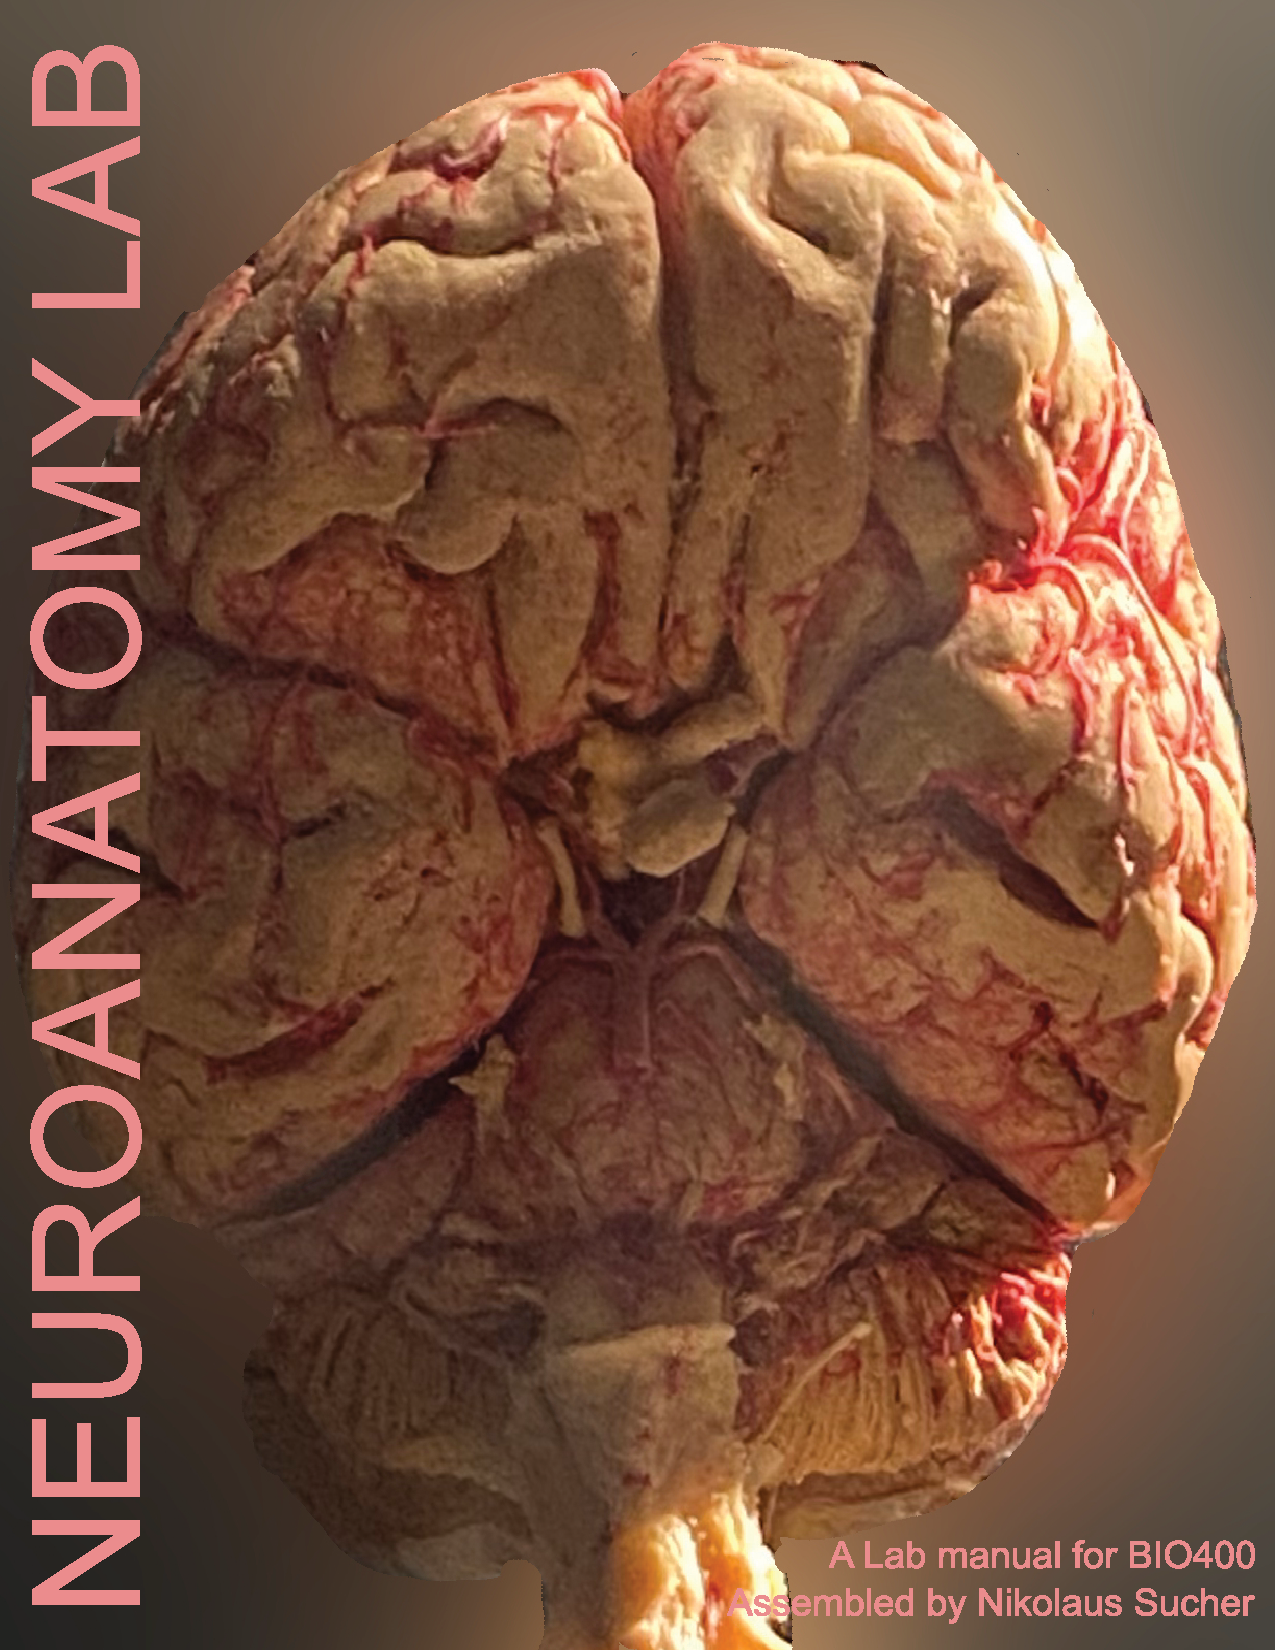
\includegraphics[width=0.7\linewidth]{neuroanatomy_lab_brain_cover} \end{center}

This work is licensed under the \href{https://creativecommons.org/licenses/by-sa/3.0/deed.en}{Creative Commons Attribution-Share Alike 3.0 Unported} United States License.

\hypertarget{acknowledgements}{%
\chapter*{Acknowledgements}\label{acknowledgements}}
\addcontentsline{toc}{chapter}{Acknowledgements}

The creation of this laboratory manual was greatly facilitated and owes a major debt to \href{https://www.wikipedia.org}{Wikipedia} and its large number of voluntary contributors. I very liberally copied from many Wikipedia pages and then remixed, edited, adapted and added text. With your continued support and help this book can only get better over time. I urge you to email me with your criticisms and suggestions at \href{mailto:nsucher@salemstate.edu}{\nolinkurl{nsucher@salemstate.edu}} This book is made available as an open educational resource under \href{https://creativecommons.org/licenses/by-sa/3.0/deed.en}{Creative Commons Attribution-Share Alike 3.0 Unported} United States License for others to do as I did and improve and adapt to specific requirements. I am grateful for the support provided by the Salem State University's OER initiative.

\hypertarget{neurons-and-glia}{%
\chapter{Neurons And Glia}\label{neurons-and-glia}}

\hypertarget{development-of-the-nervous-system}{%
\chapter{Development Of The Nervous System}\label{development-of-the-nervous-system}}

In this laboratory session, we will study the anatomy of the human mesencephalon. Below, you will be presented with a number of figures and asked to label or color certain structures in each figure.

\hypertarget{surface-anatomy-of-the-brain}{%
\chapter{Surface Anatomy Of The Brain}\label{surface-anatomy-of-the-brain}}

In this laboratory session, we will study the surface anatomy of the human brain. Below, you will be presented with a number of figures and asked to label or color certain structures in each figure.

\hypertarget{a-dorsal-view-of-a-human-brain.}{%
\section{A Dorsal View Of A Human Brain.}\label{a-dorsal-view-of-a-human-brain.}}

\begin{enumerate}
\def\labelenumi{\arabic{enumi}.}
\tightlist
\item
  Write ``LH`` over the left hemisphere and ``RH`` over the right
hemisphere in figure 1 below.
\item
  Write ``ANTERIOR' and ``POSTERIOR`` next to the arrowhead pointing
in the corresponding direction: 

\item
  Mark the longitudinal cerebral fissure with a sequence of ``x'''s

\end{enumerate}



\begin{figure}

{\centering 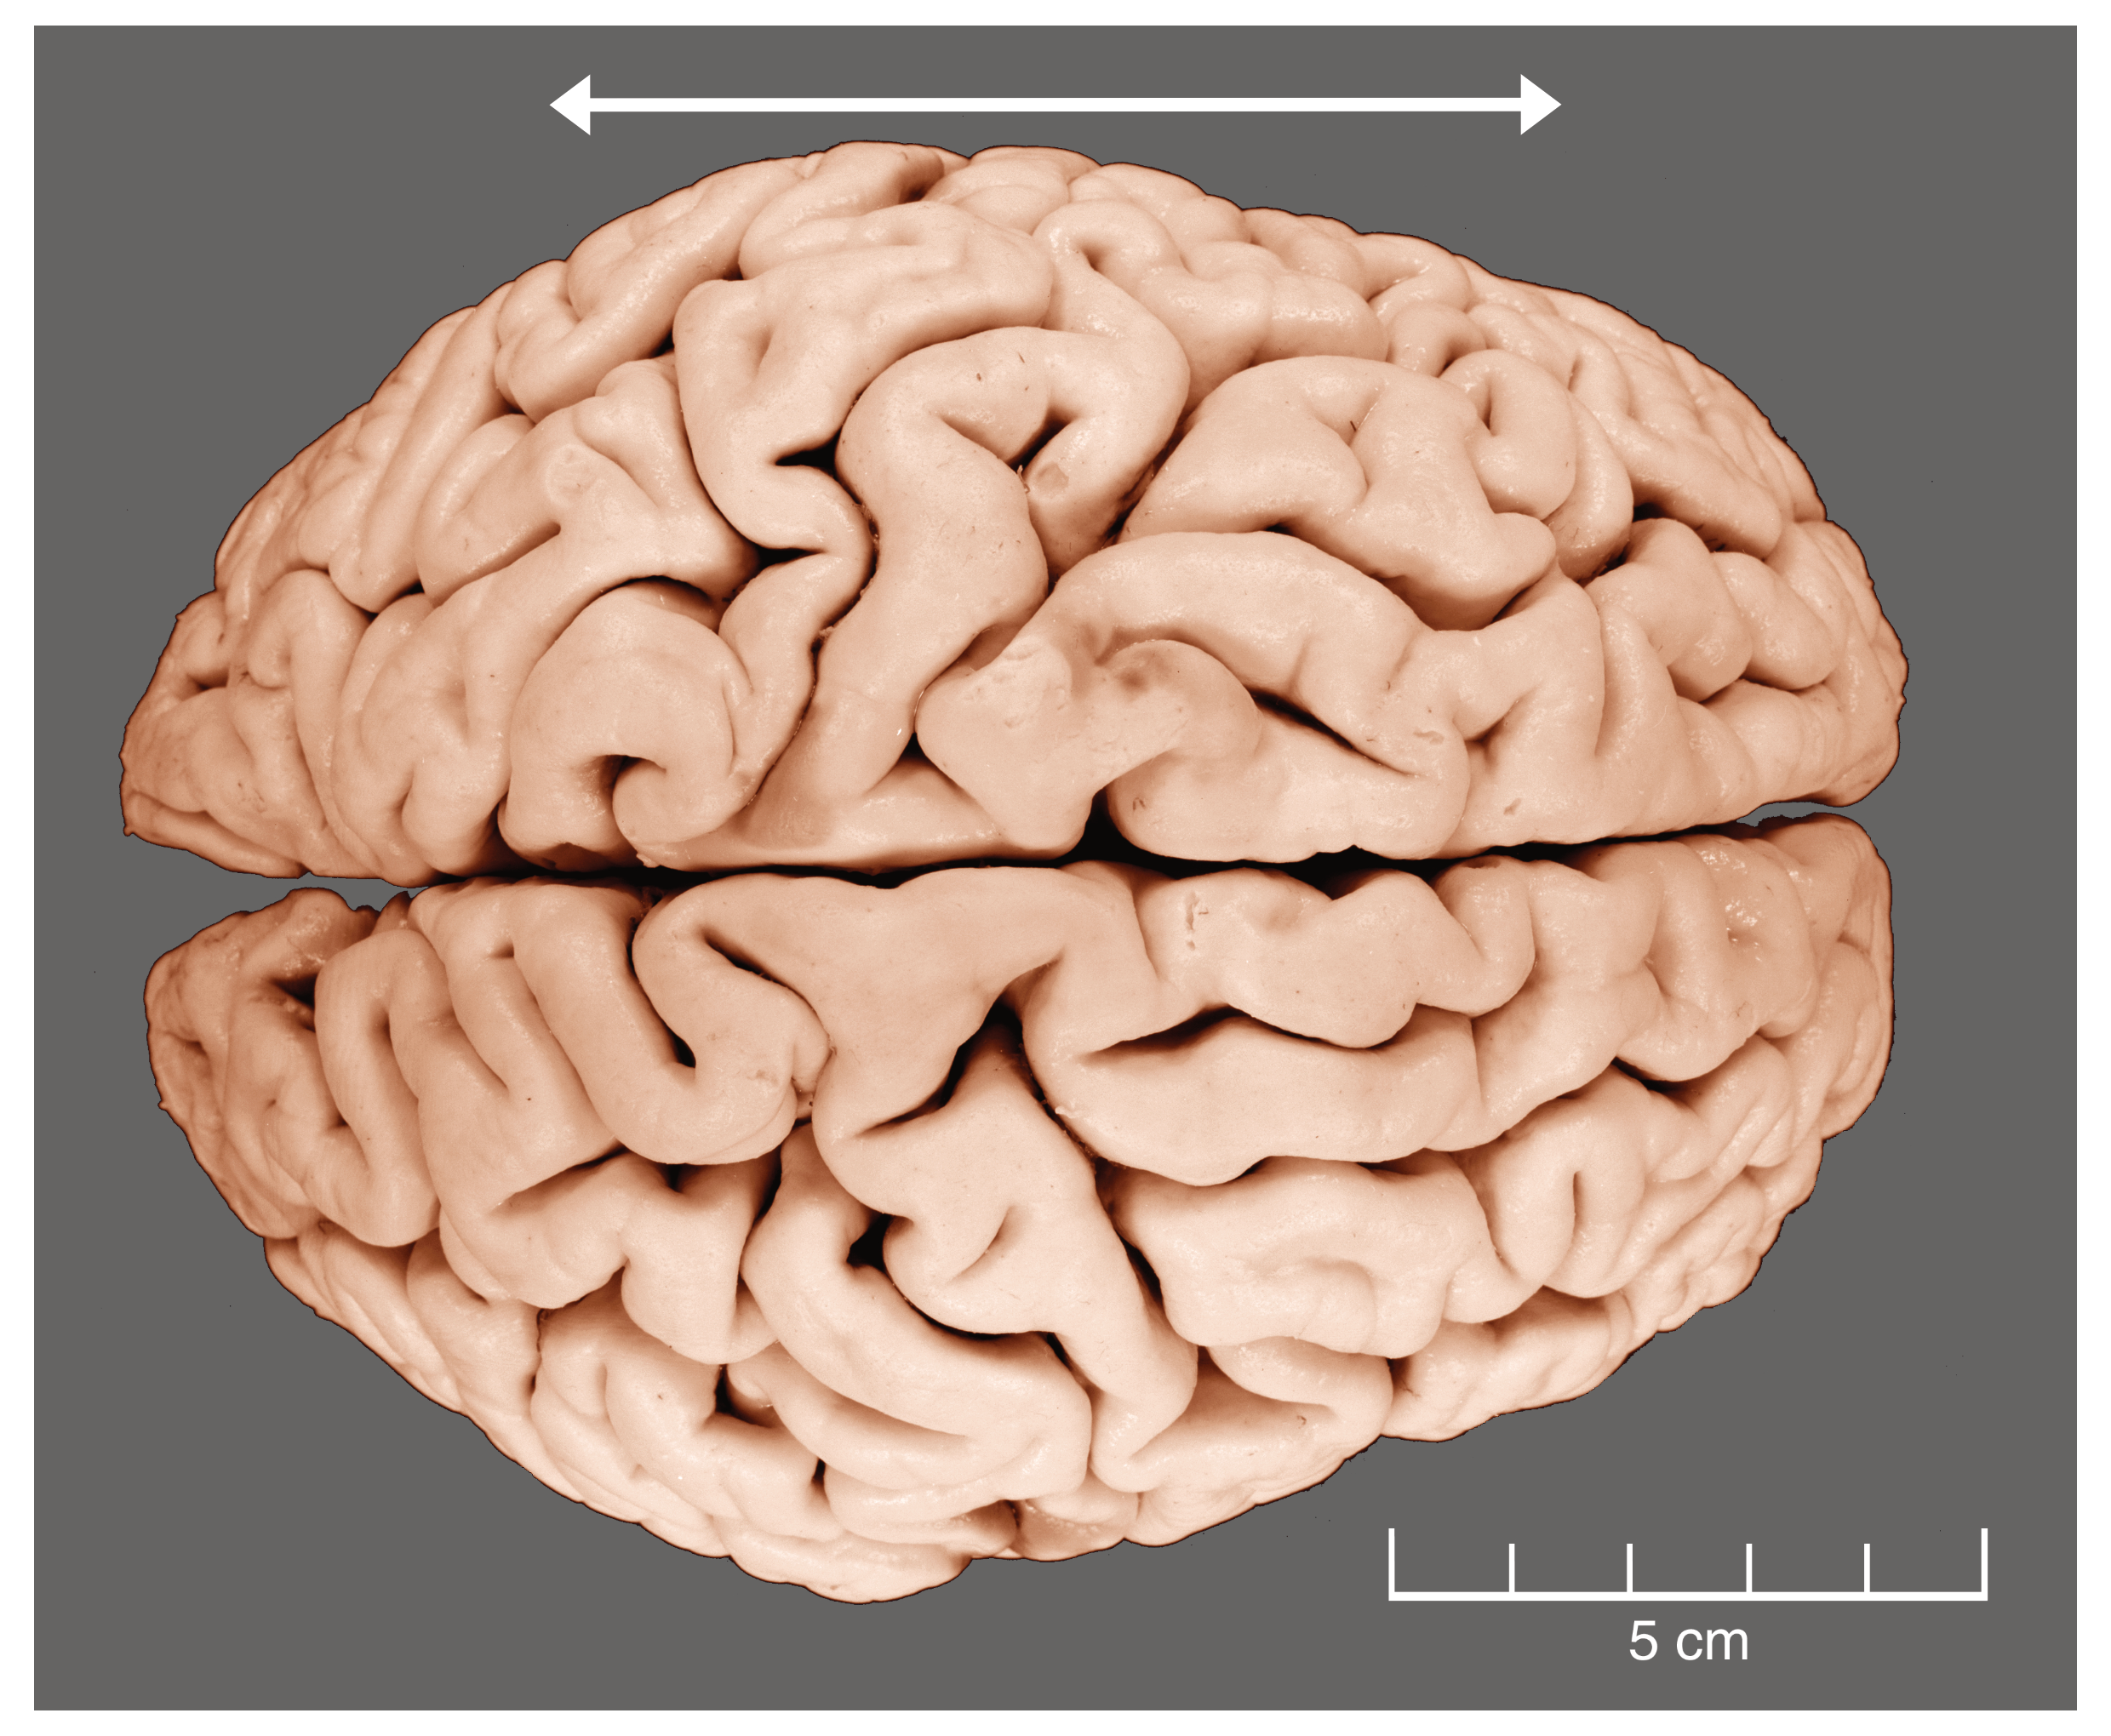
\includegraphics[width=0.7\linewidth]{./figures/cns/human_brain_dorsal} 

}

\caption{A dorsal view of a human brain.}\label{fig:hbdorsal}
\end{figure}

\hypertarget{a-dorso-lateral-view-of-a-human-brain.}{%
\section{A Dorso-Lateral View Of A Human Brain.}\label{a-dorso-lateral-view-of-a-human-brain.}}

\begin{enumerate}
\def\labelenumi{\arabic{enumi}.}
\tightlist
\item
  Write ``ANTERIOR' and ``POSTERIOR`` next to the arrowhead pointing
in the corresponding direction 

\item
  Trace the Sylvian fissure using a black marker
\item
  Trace the central sulcus from the midline to the Sylvian fissure using a black marker
\end{enumerate}



\begin{figure}

{\centering \includegraphics[width=0.7\linewidth]{./figures/cns/human_brain_dorsal_lateral} 

}

\caption{A dorso-lateral view of a human brain.}\label{fig:hbdl}
\end{figure}

\hypertarget{a-lateral-view-of-a-human-brain.}{%
\section{A Lateral View Of A Human Brain.}\label{a-lateral-view-of-a-human-brain.}}

\begin{enumerate}
\def\labelenumi{\arabic{enumi}.}
\tightlist
\item
  Write ``ANTERIOR' and ``POSTERIOR`` next to the arrowhead pointing
in the corresponding direction 

\item
  Write ``DORSAL`` and ``VENTRAL`` next to the arrowhead pointing
in the corresponding direction 

\item
  Write ``CEREBRUM`` and ``CEREBELLUM`` next to the corresponding structures
\item
  rite ``BRAINSTEM`` next to the corresponding structure

\item
  Write ``OLFACTORY BULB`` next to the corresponding structure

\end{enumerate}



\begin{figure}

{\centering 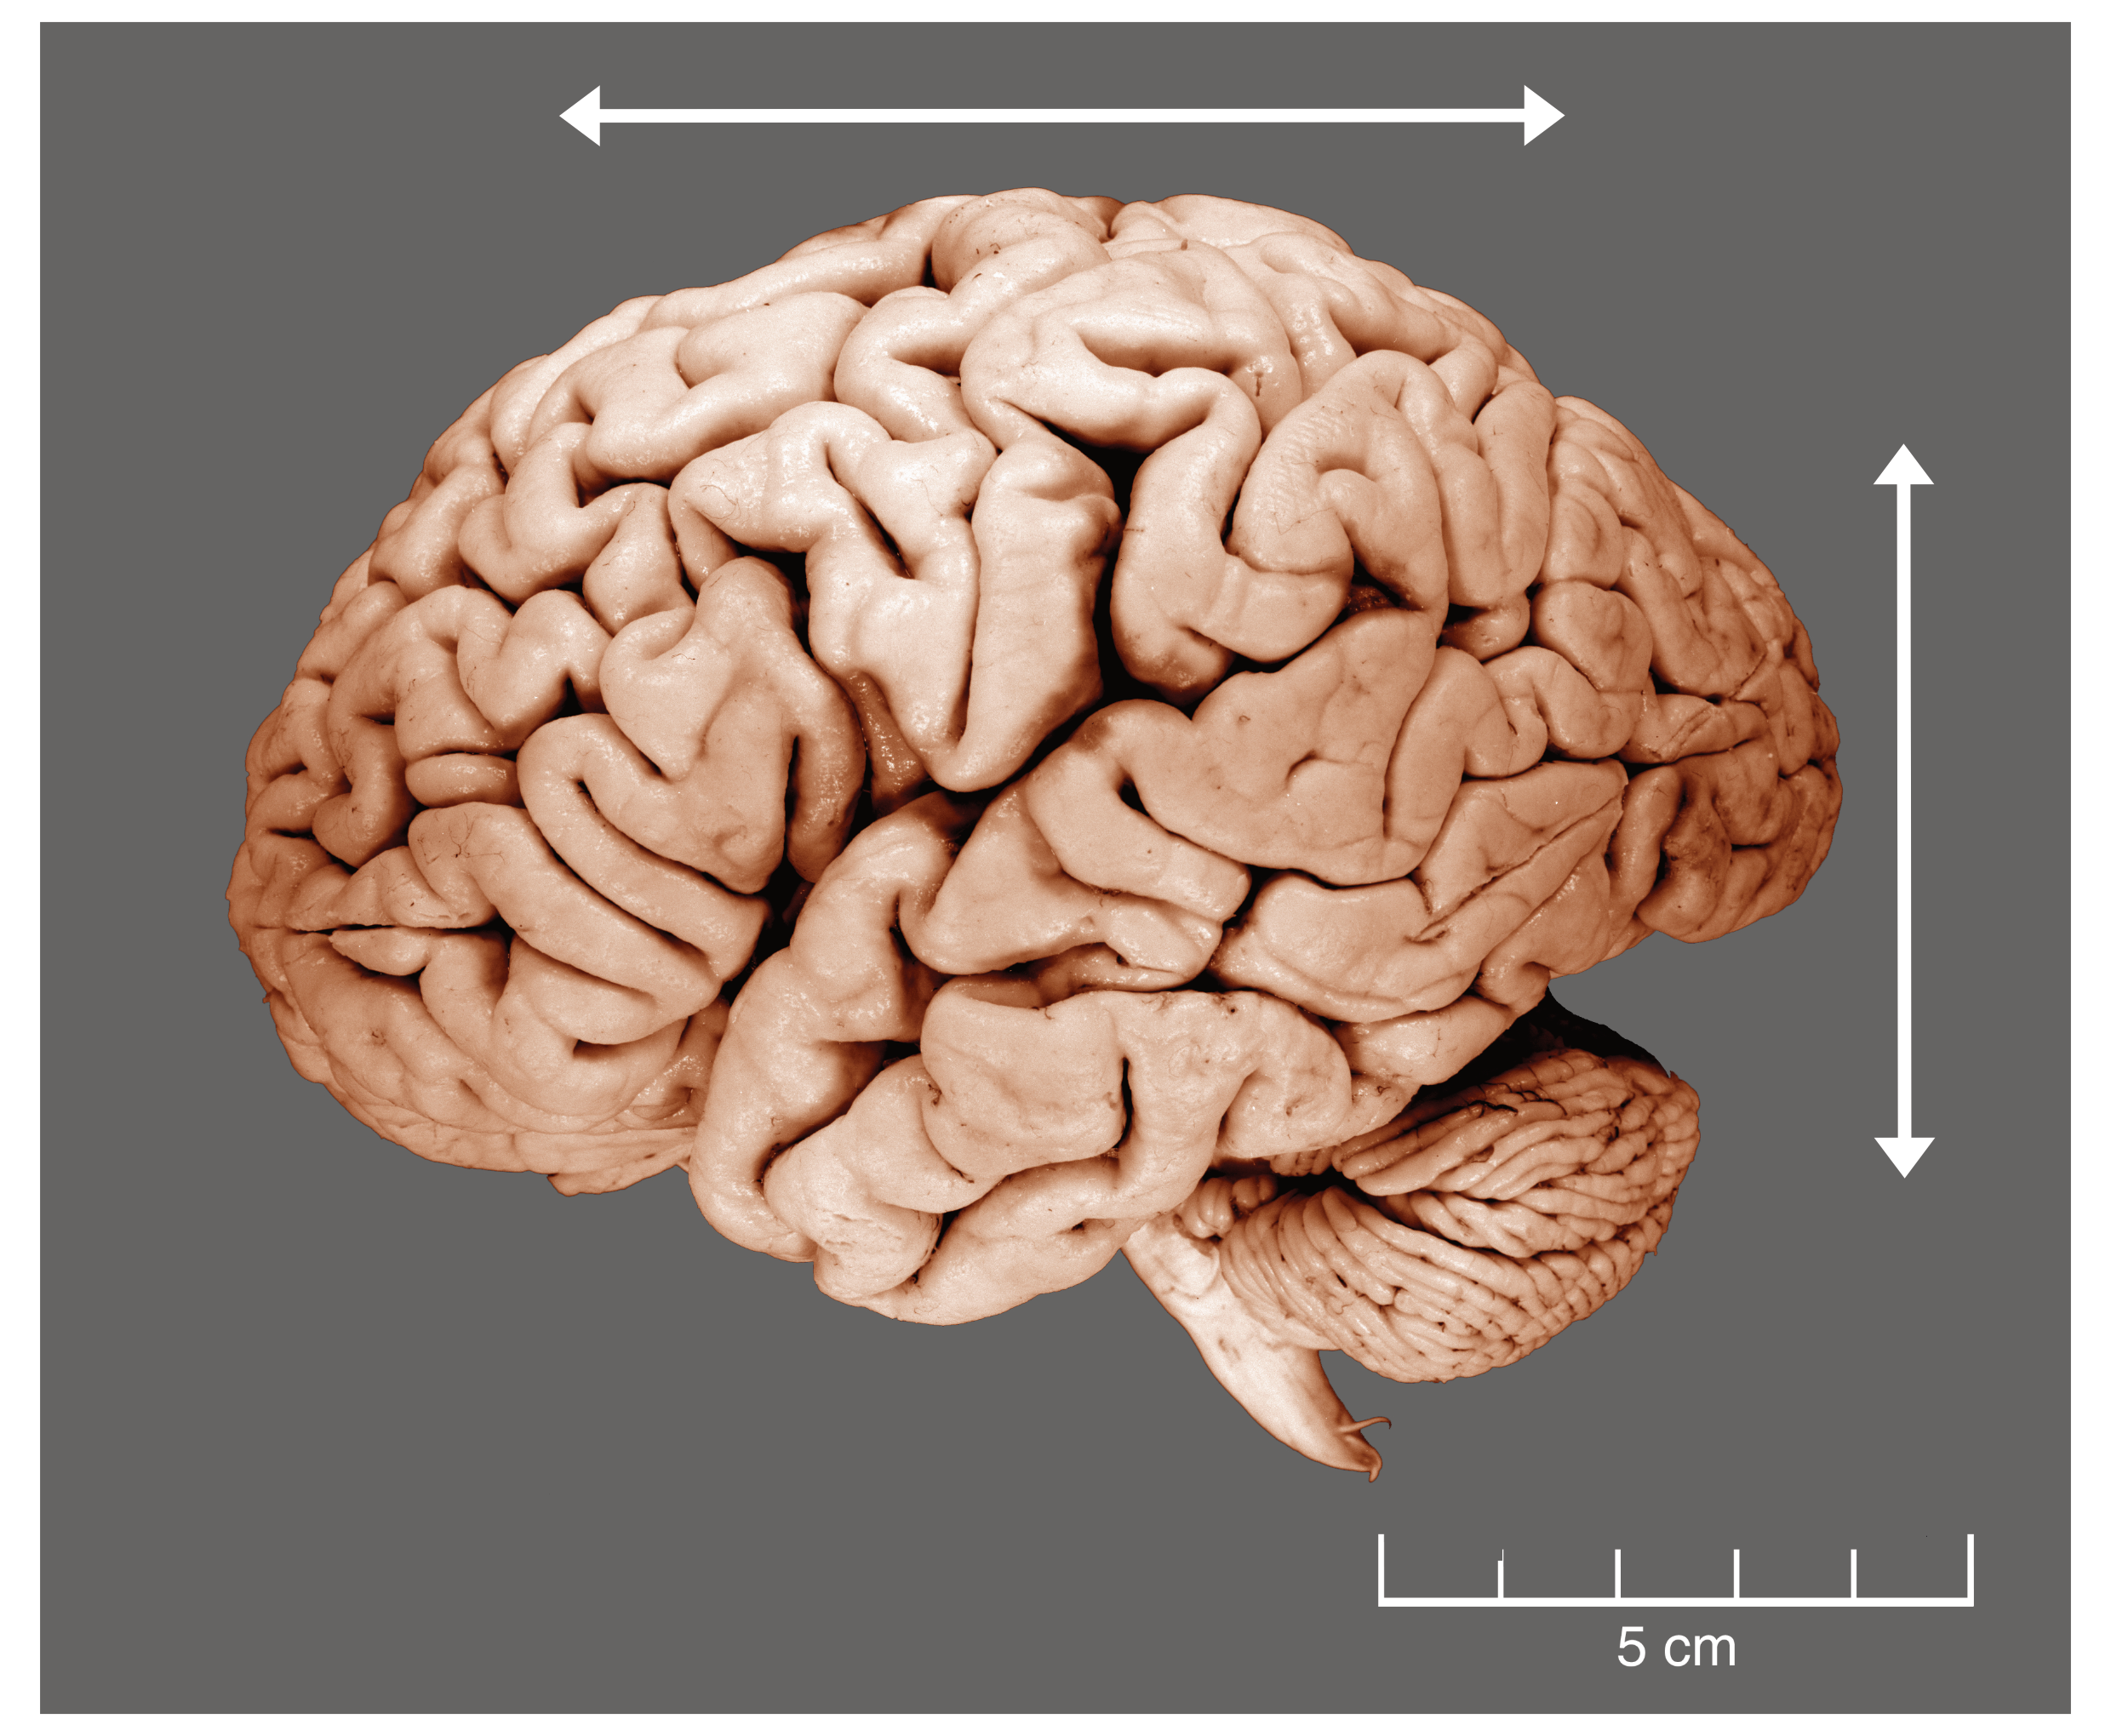
\includegraphics[width=0.7\linewidth]{./figures/cns/human_brain_lateral} 

}

\caption{A lateral view of a human brain.}\label{fig:hbl}
\end{figure}

\hypertarget{a-ventral-view-of-a-human-brain.}{%
\section{A Ventral View Of A Human Brain.}\label{a-ventral-view-of-a-human-brain.}}

\begin{enumerate}
\def\labelenumi{\arabic{enumi}.}
\tightlist
\item
  Write ``LH`` over the left hemisphere and ``RH` over the right
hemisphere in figure 1 below.
\item
  Write ``LCblH`` over the left hemisphere of the cerebellum
and ``RCblH` over the right cerebellar hemisphere in the figure below.
\item
  Write ``Pons`` over the corresponding structure in the figure below.
\item
  Write ``MO`` denoting the medulla oblongata over the corresponding
structure in the figure below.
\item
  Write ``ANTERIOR' and ``POSTERIOR`` next to the arrowhead pointing
in the corresponding direction.

\end{enumerate}



\begin{figure}

{\centering 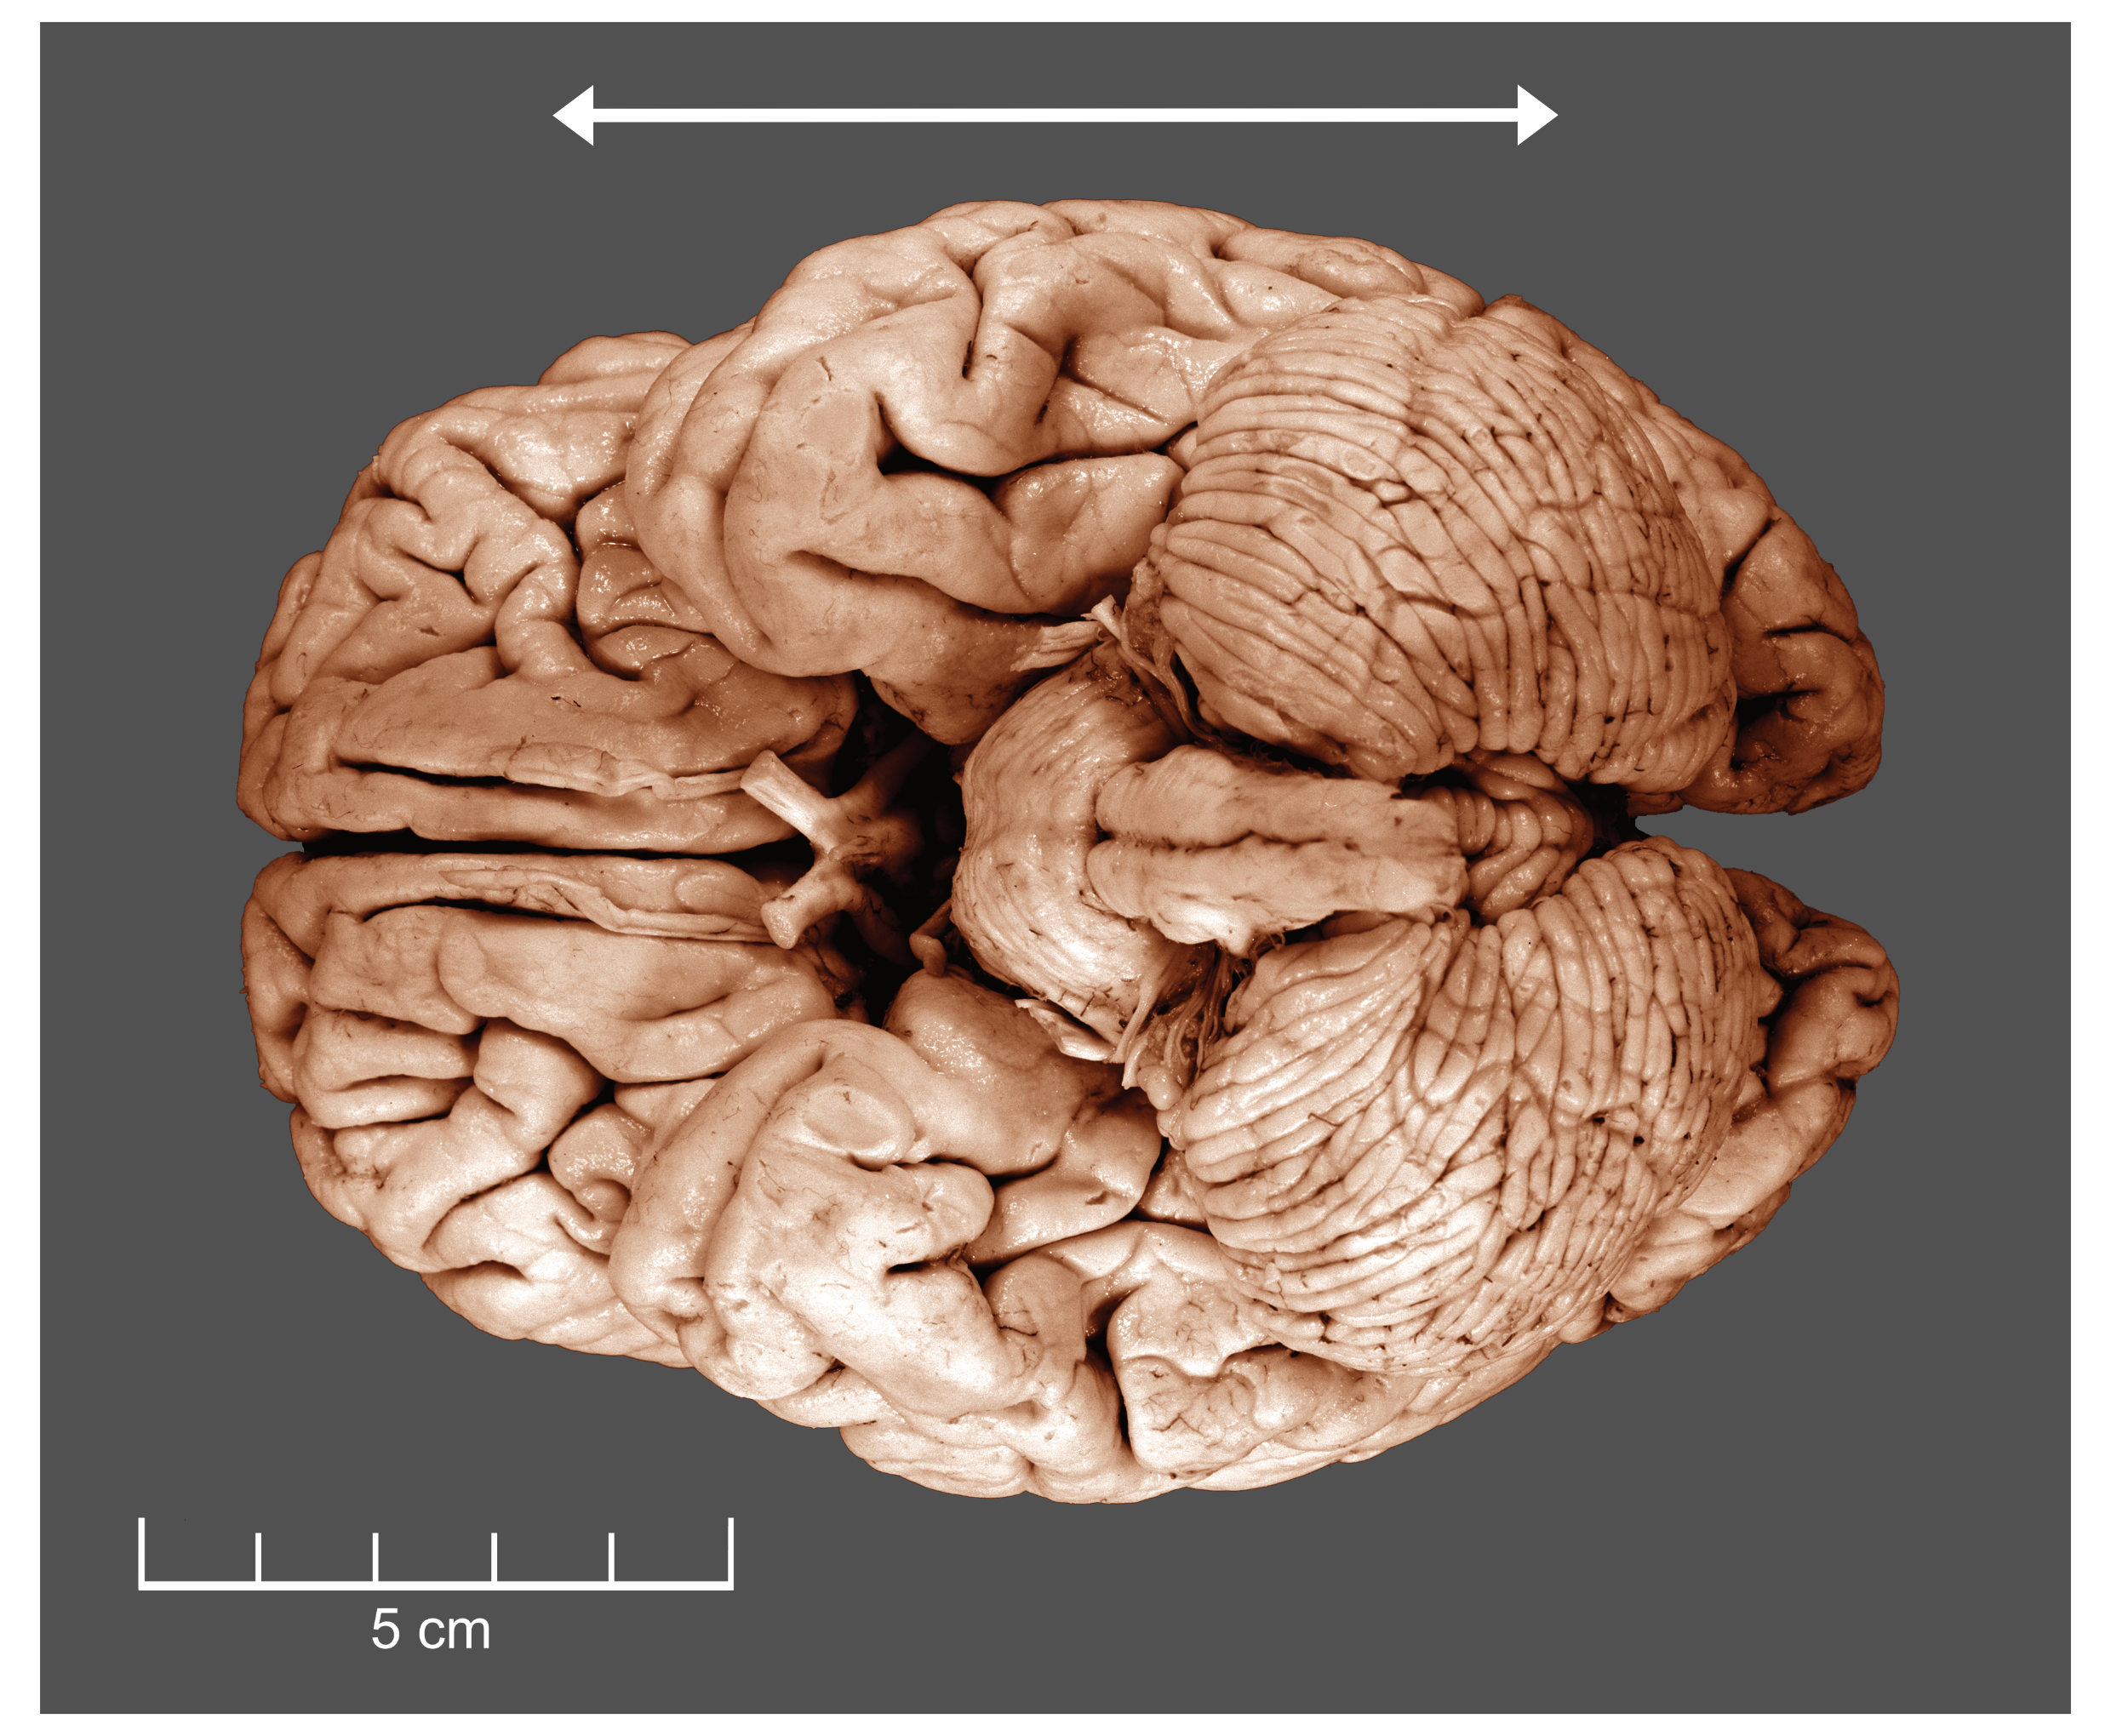
\includegraphics[width=0.7\linewidth]{./figures/cns/human_brain_ventral} 

}

\caption{A ventral view of a human brain.}\label{fig:hbv}
\end{figure}

\hypertarget{a-lateral-view-of-the-human-brain.}{%
\section{A Lateral View Of The Human Brain.}\label{a-lateral-view-of-the-human-brain.}}

\begin{enumerate}
\def\labelenumi{\arabic{enumi}.}
\tightlist
\item
  Color the frontal lobe red
\item
  Color the temporal lobe green
\item
  Color the parietal lobe yellow
\item
  Color the occipital lobe blue
\item
  Mark the central sulcus with a sequence of ``o``'s
\item
  Mark the Sylvian fissure with a sequence of ``x'''s

\end{enumerate}



\begin{figure}

{\centering 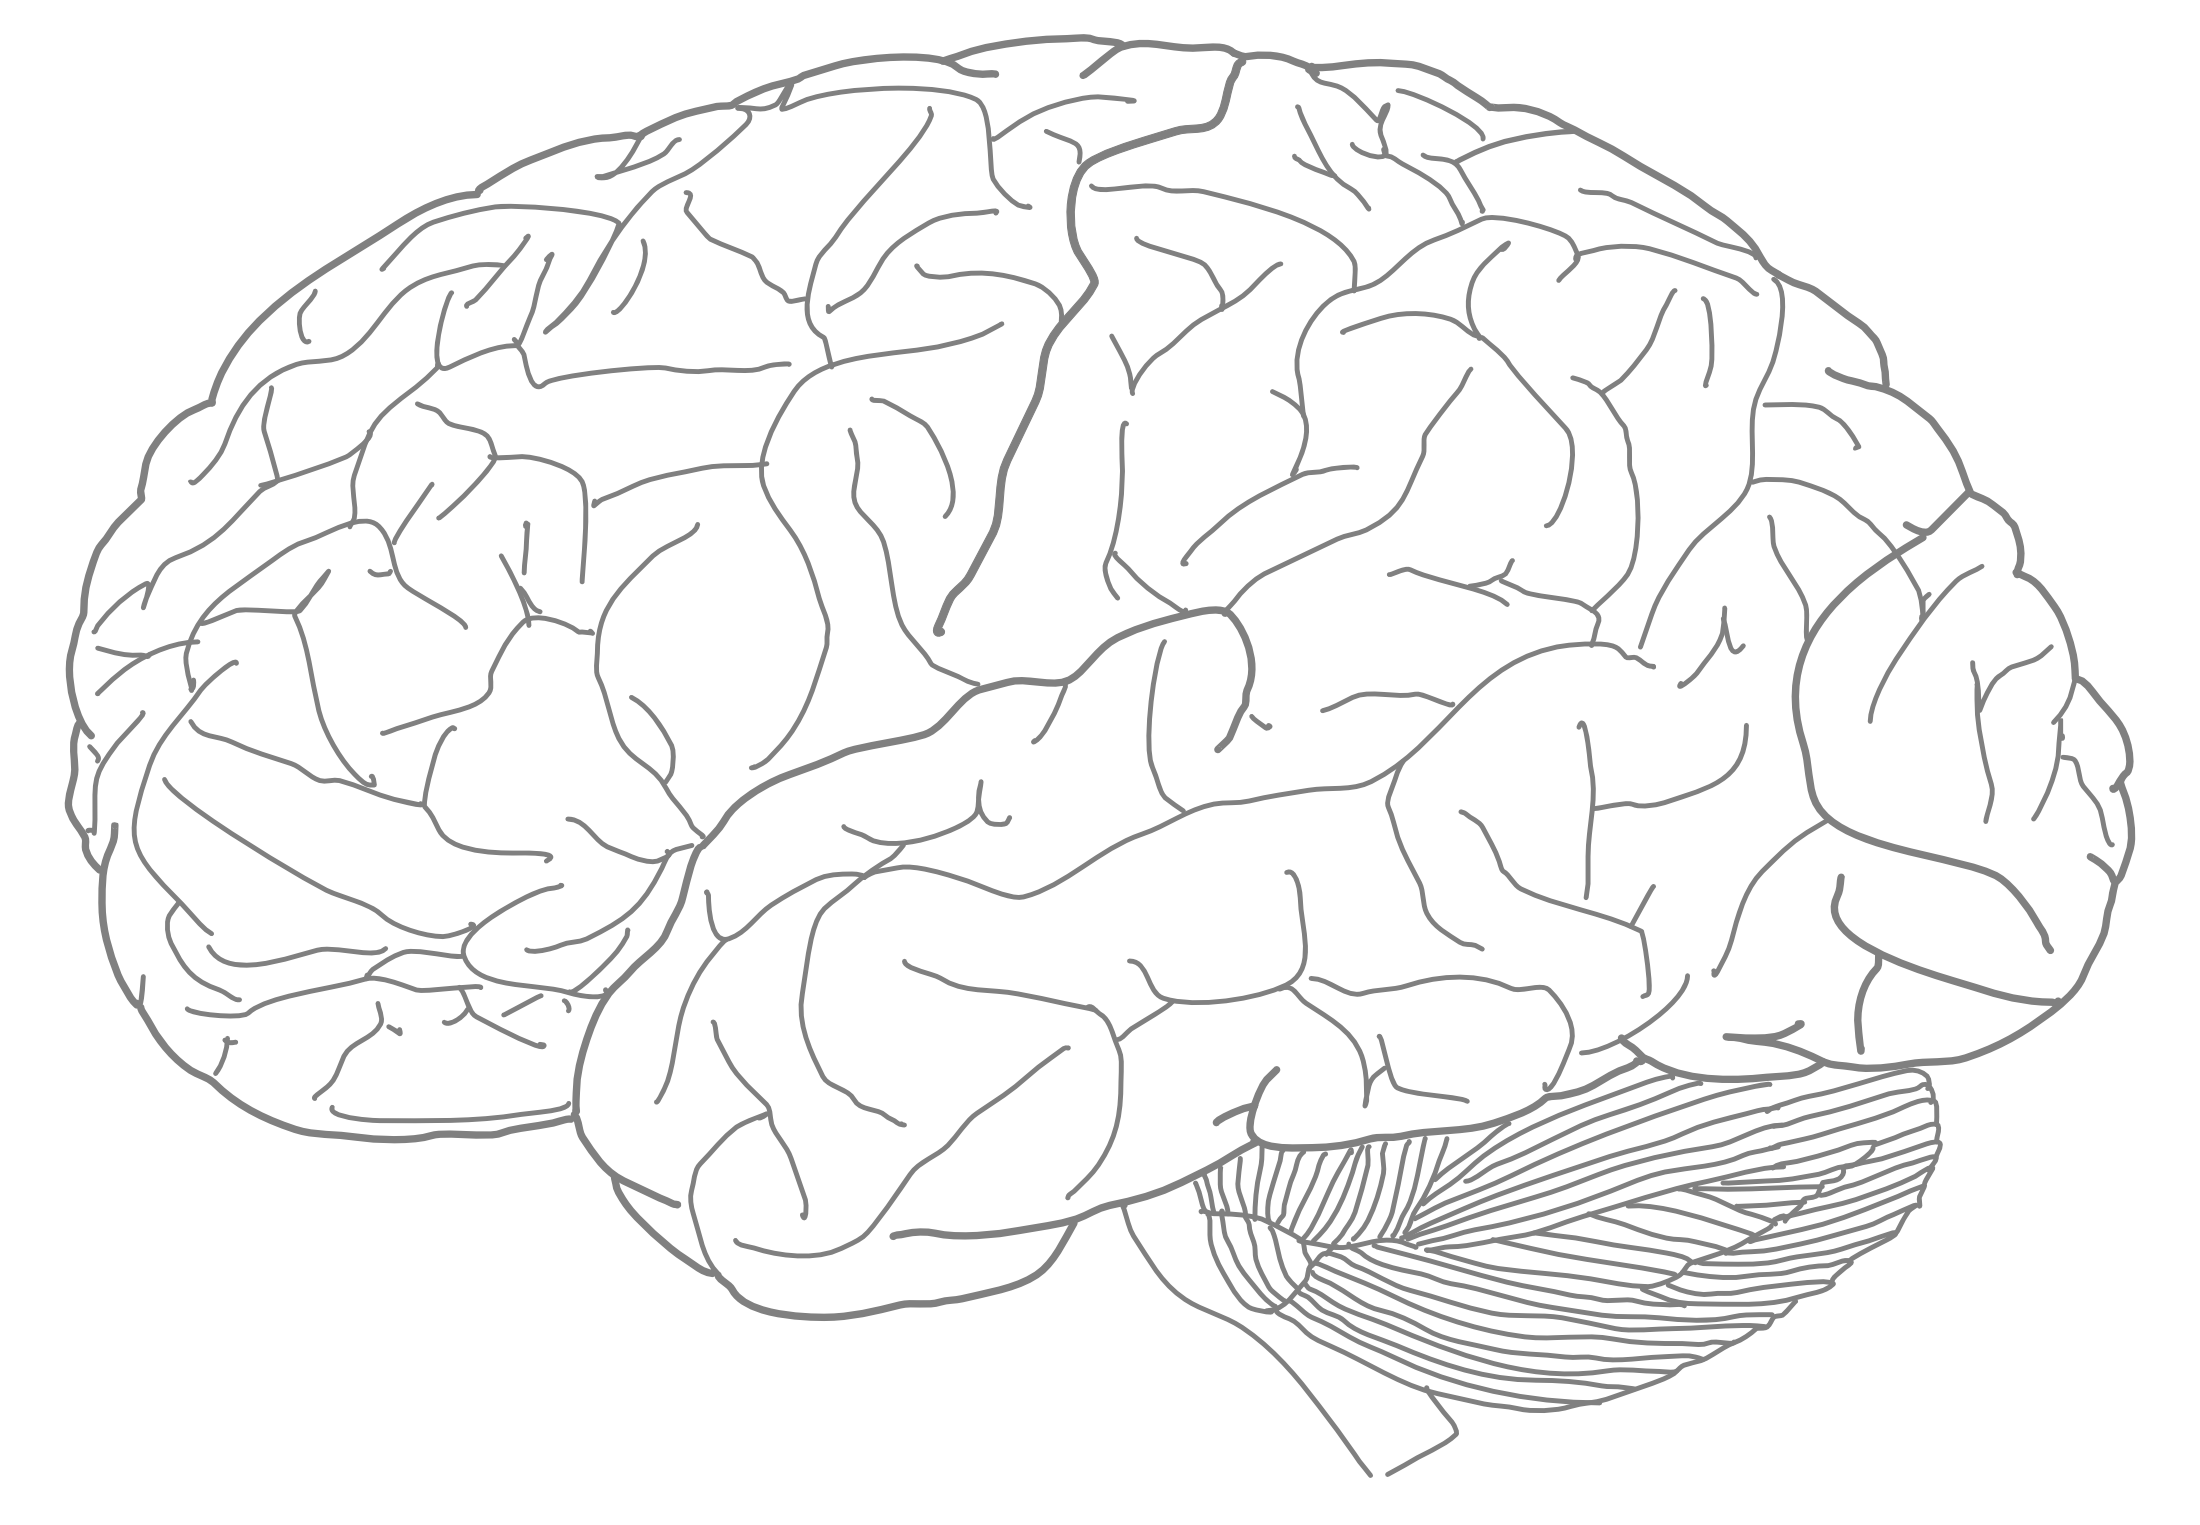
\includegraphics[width=0.7\linewidth]{./figures/cns/brain_for_labeling_lobes} 

}

\caption{A lateral view of the major lobes of the human brain.}\label{fig:bfll}
\end{figure}

\begin{enumerate}
\def\labelenumi{\arabic{enumi}.}
\tightlist
\item
  Mark the central sulcus with a sequence of ``o``'s.
\item
  Mark the Sylvian fissure with a sequence of ``x'''s.
\item
  Color the precentral gyrus red.
\item
  Color the postcentral gyrus green.
\item
  Color the superior temporal gyrus blue.

\end{enumerate}



\begin{figure}

{\centering 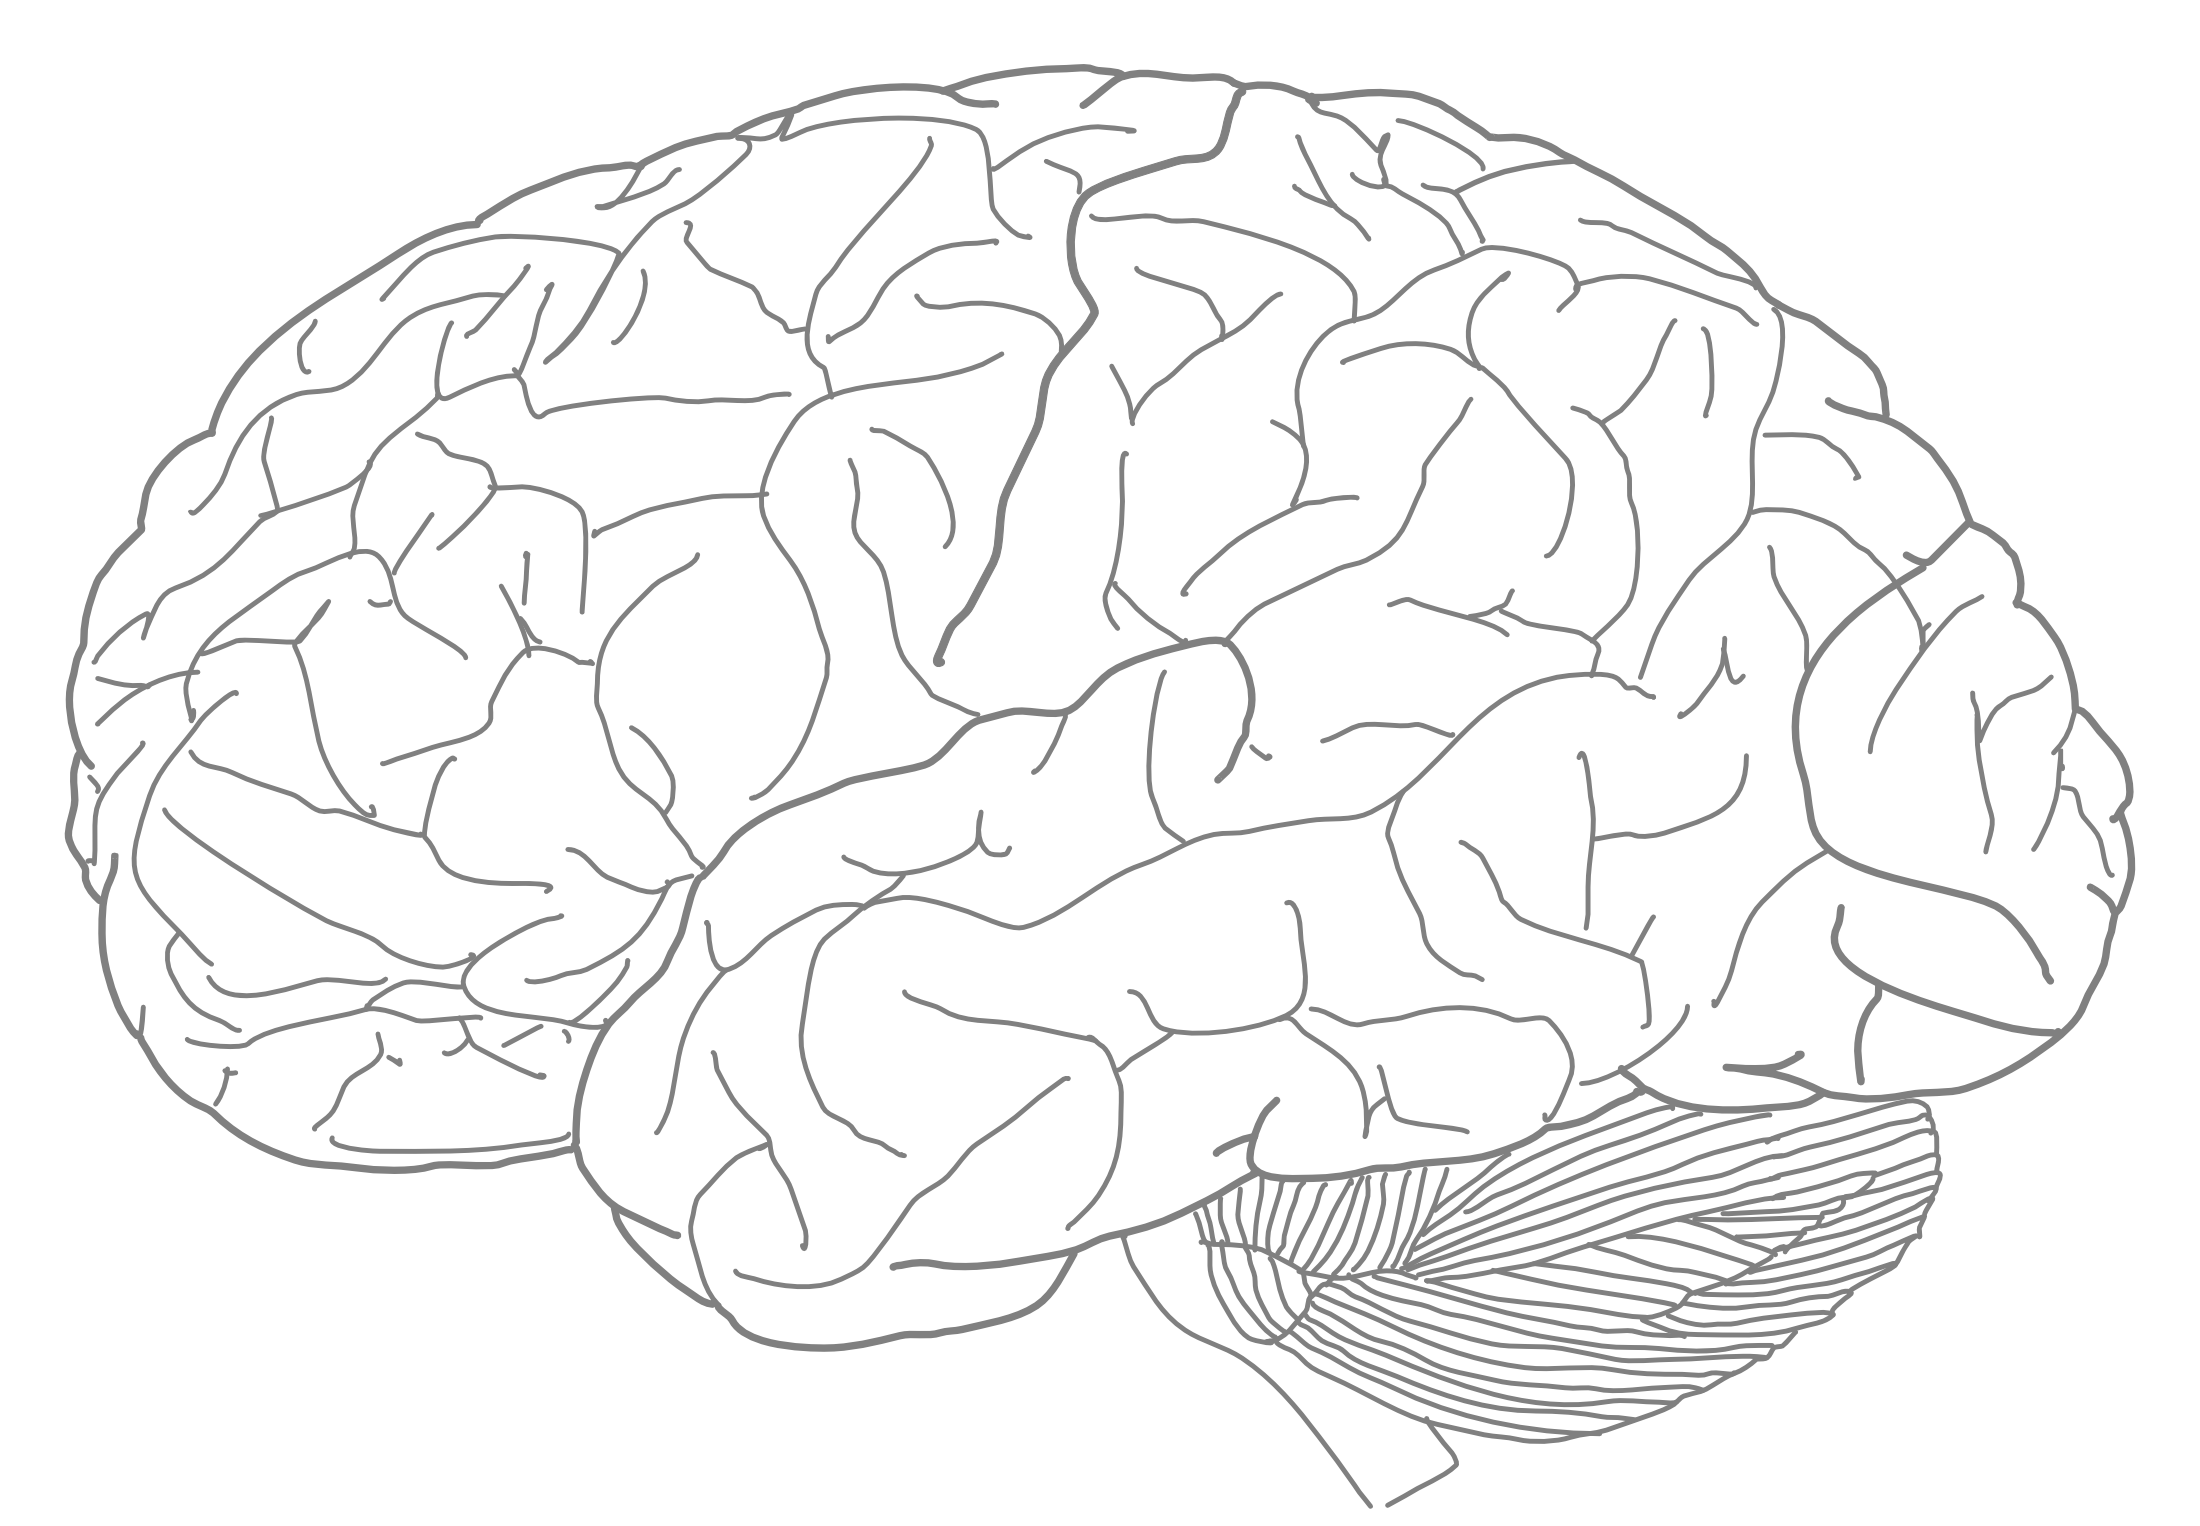
\includegraphics[width=0.7\linewidth]{./figures/cns/brain_for_labeling_gyri} 

}

\caption{A lateral view of the major gyri of the human brain.}\label{fig:bflg}
\end{figure}

\hypertarget{a-medial-view-of-the-human-brain.}{%
\section{A Medial View Of The Human Brain.}\label{a-medial-view-of-the-human-brain.}}

\begin{enumerate}
\def\labelenumi{\arabic{enumi}.}
\tightlist
\item
  Color the septum pellucidum yellow
\item
  Color the thalamus blue
\item
  Color the hypothalamus grey
\item
  Color the pons red
\item
  Color the medulla oblongata green
\item
  Color the tectum yellow
\item
  Color the tegmentum grey
\item
  Color the pineal body red

\end{enumerate}



\begin{figure}

{\centering 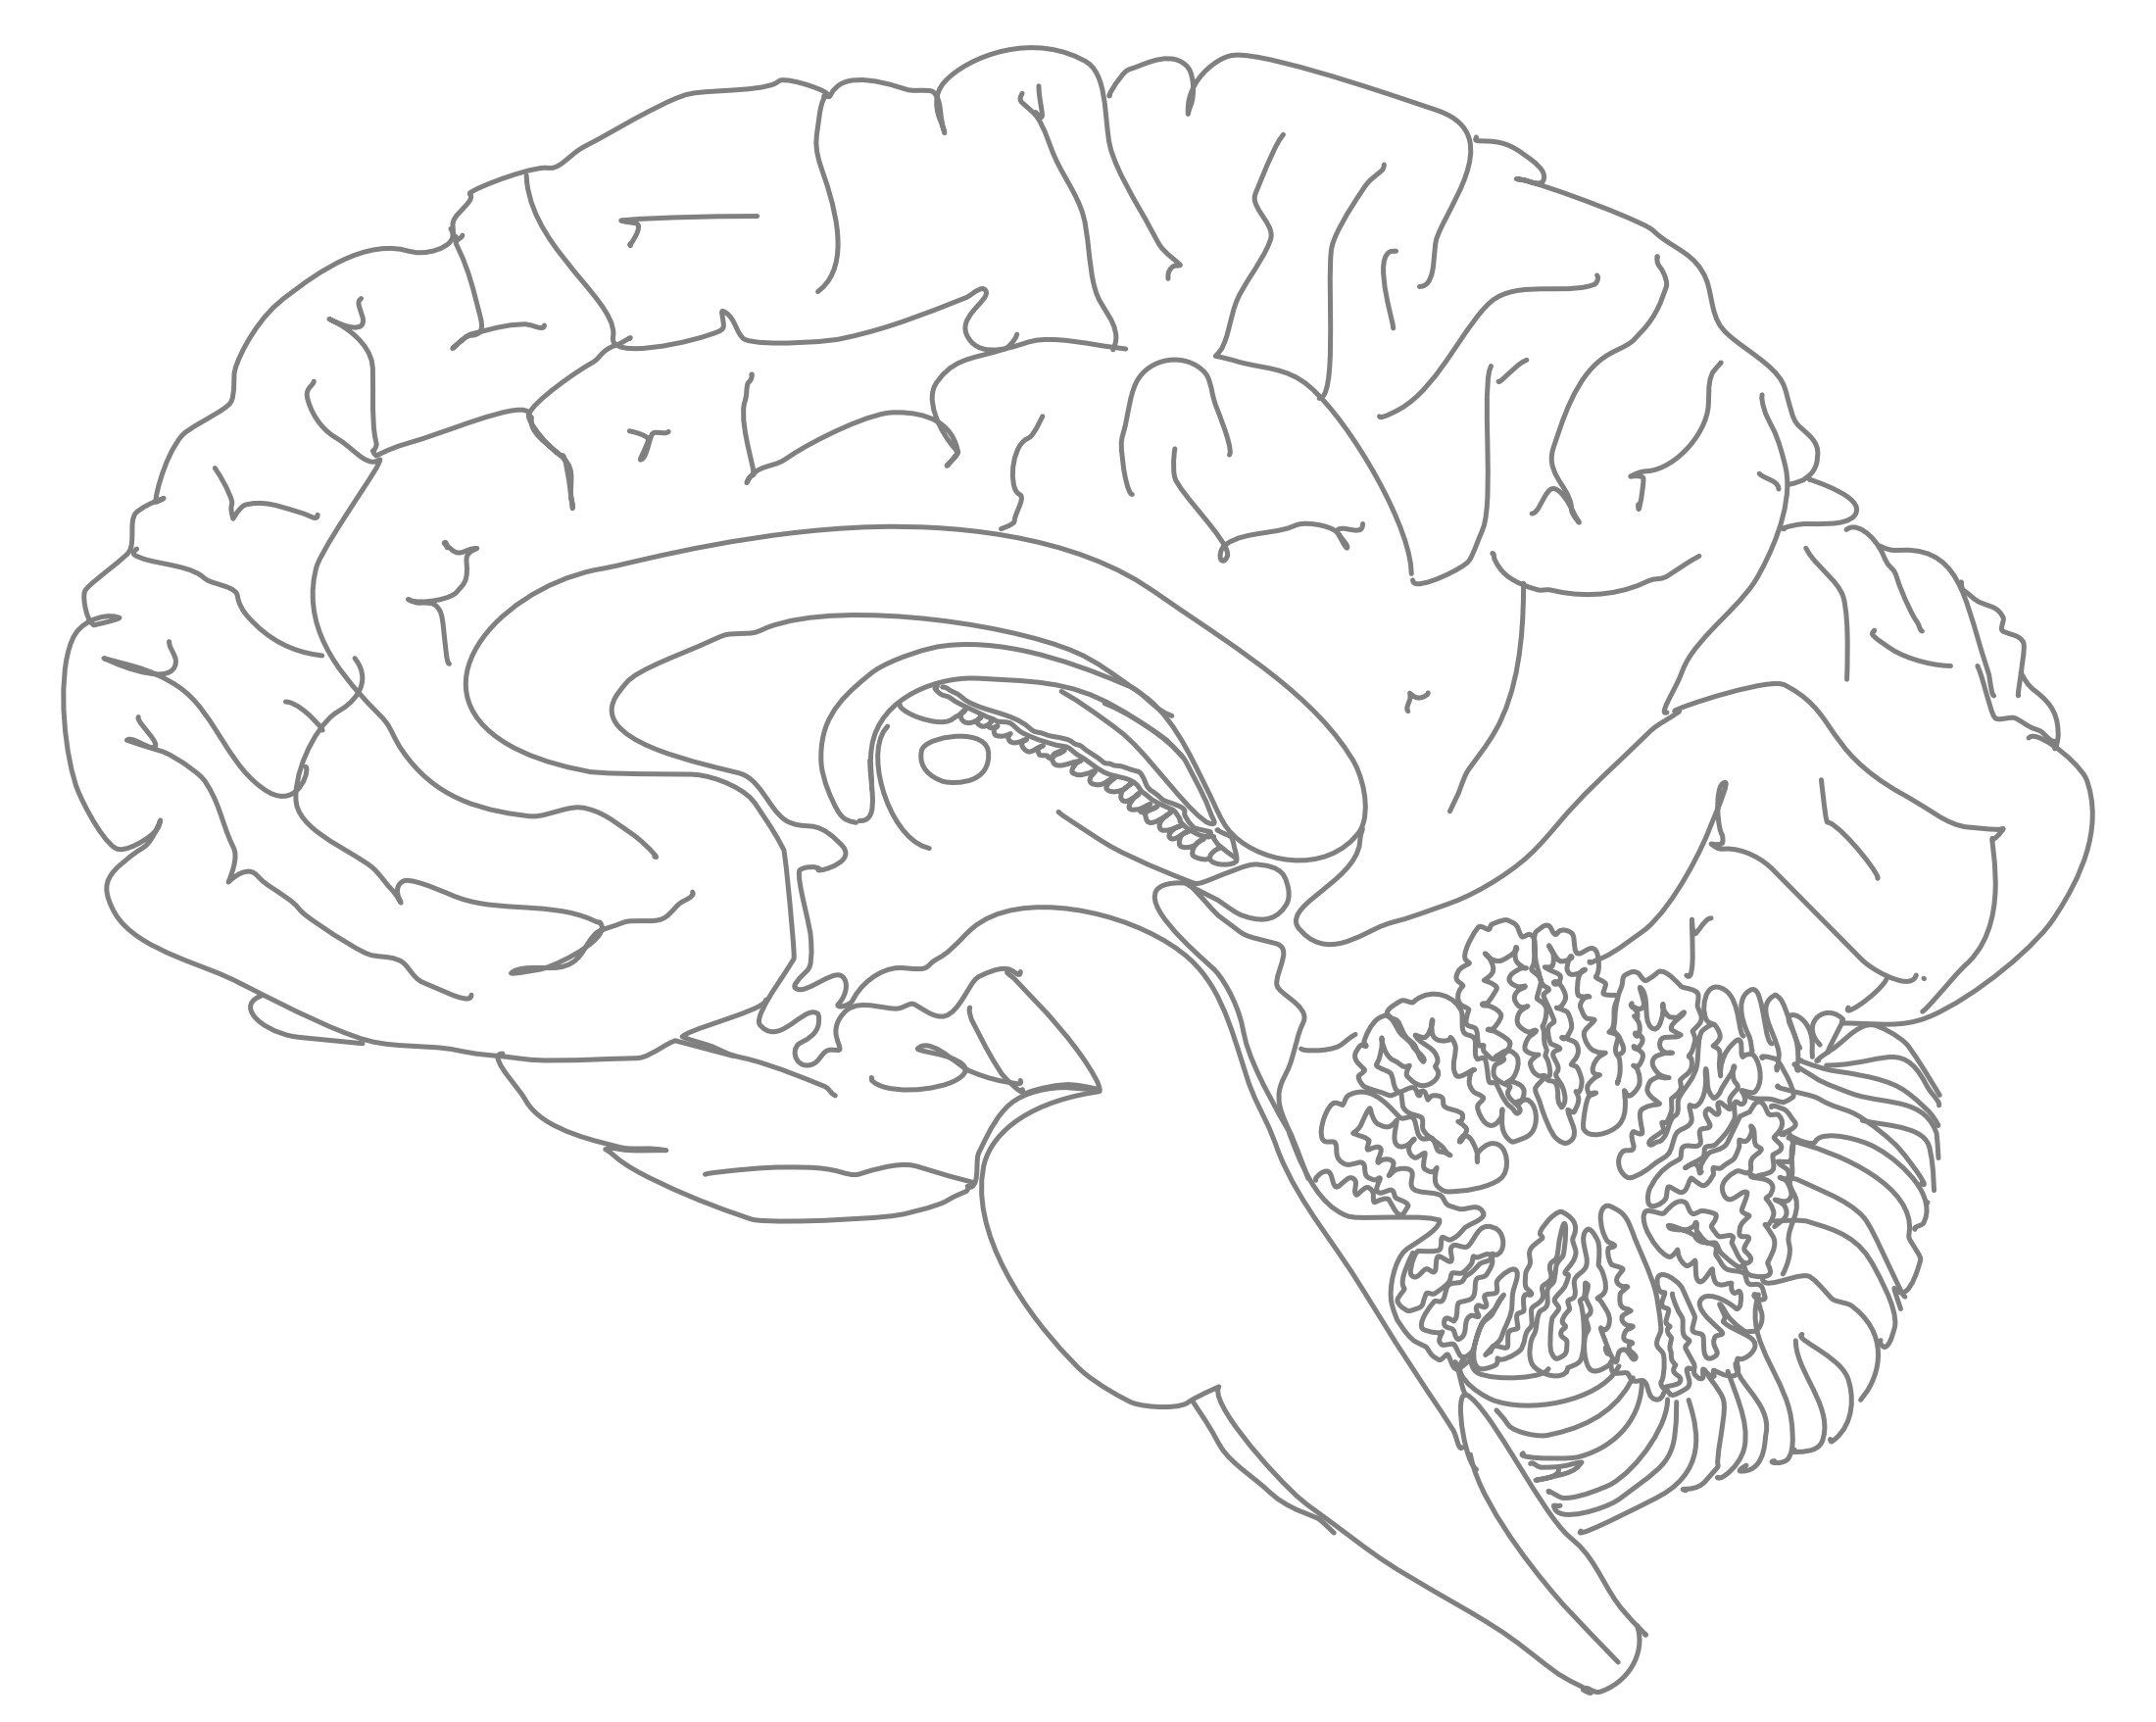
\includegraphics[width=0.7\linewidth]{./figures/cns/brain_for_labeling_medial_I} 

}

\caption{A medial view of the human brain.}\label{fig:bflm}
\end{figure}

\begin{enumerate}
\def\labelenumi{\arabic{enumi}.}
\tightlist
\item
  Color the cingulate gyrus green
\item
  Color the corpus callosum red
\item
  Color the fornix yellow
\item
  Color the olfactory bulb blue
\item
  Color the optic chiasm grey

\end{enumerate}



\begin{figure}

{\centering 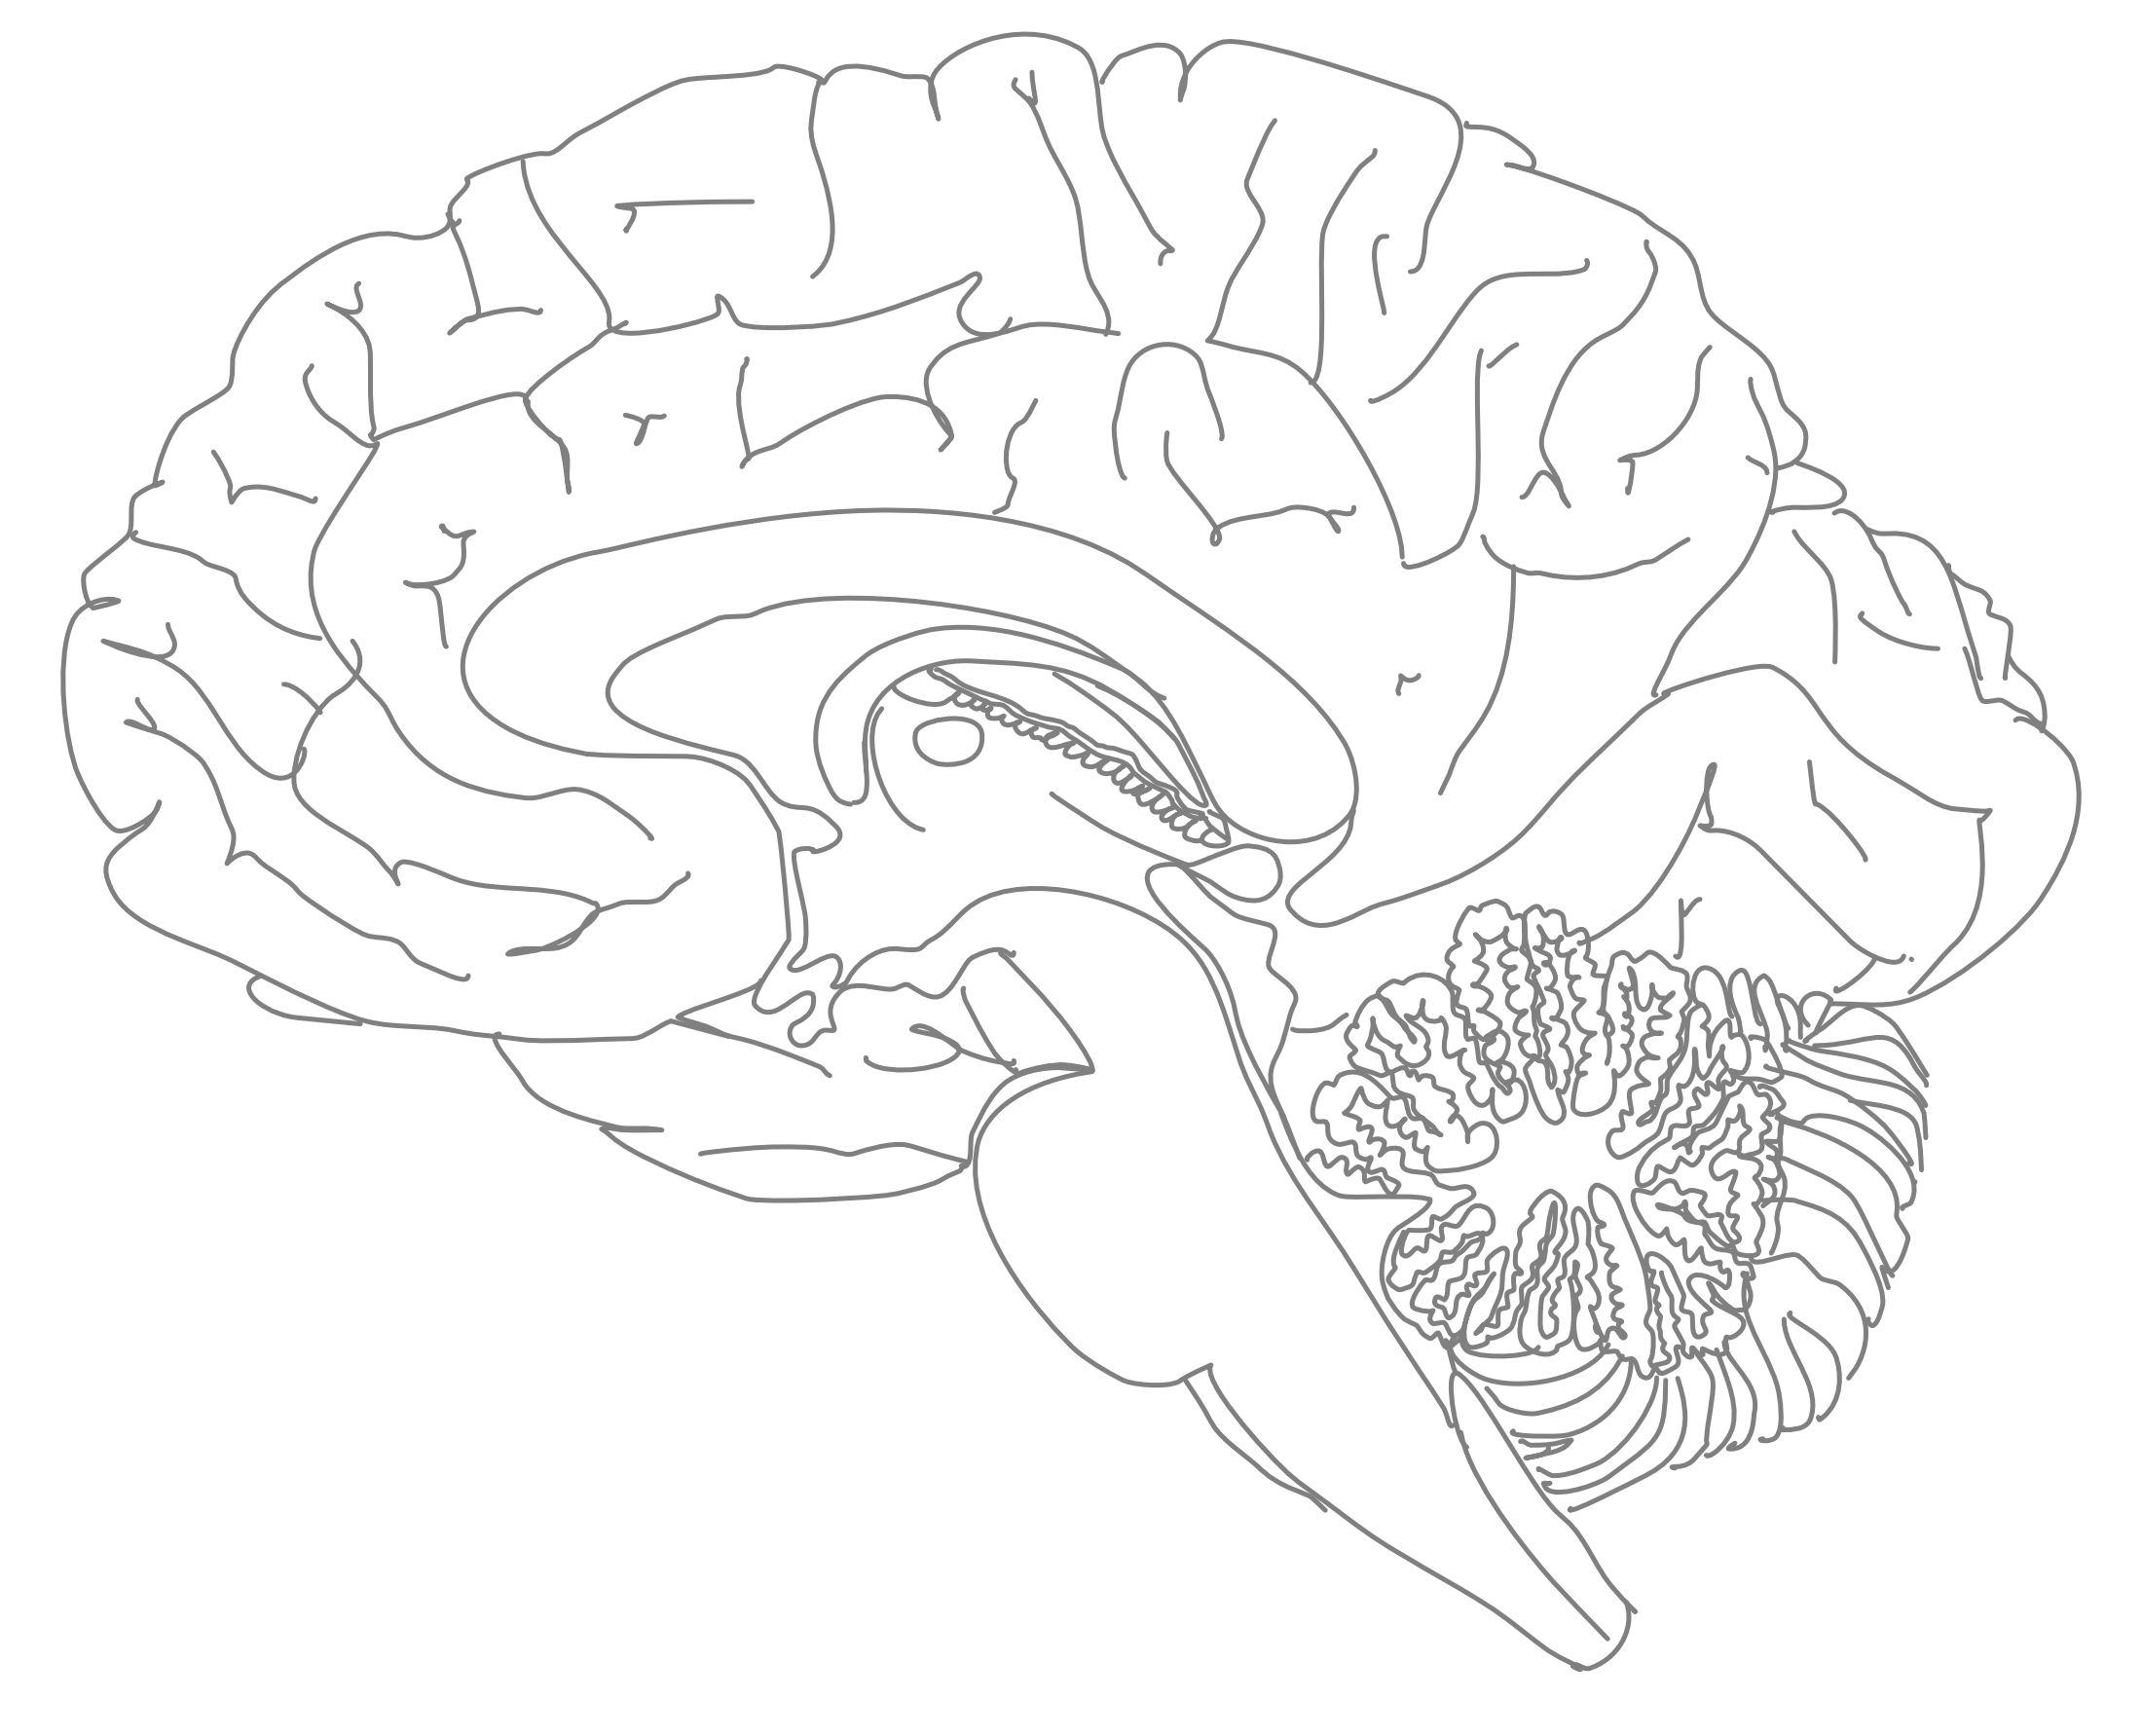
\includegraphics[width=0.7\linewidth]{./figures/cns/brain_for_labeling_medial_II} 

}

\caption{A medial view of a human brain.}\label{fig:bflmii}
\end{figure}

\begin{enumerate}
\def\labelenumi{\arabic{enumi}.}
\tightlist
\item
  Color the third ventricle green
\item
  Color the aqueduct red
\item
  Color the fourth ventricle blue
\item
  Color the spinal call yellow

\end{enumerate}

A medial view of a human brain. A medial view of a human brain.

\begin{figure}

{\centering 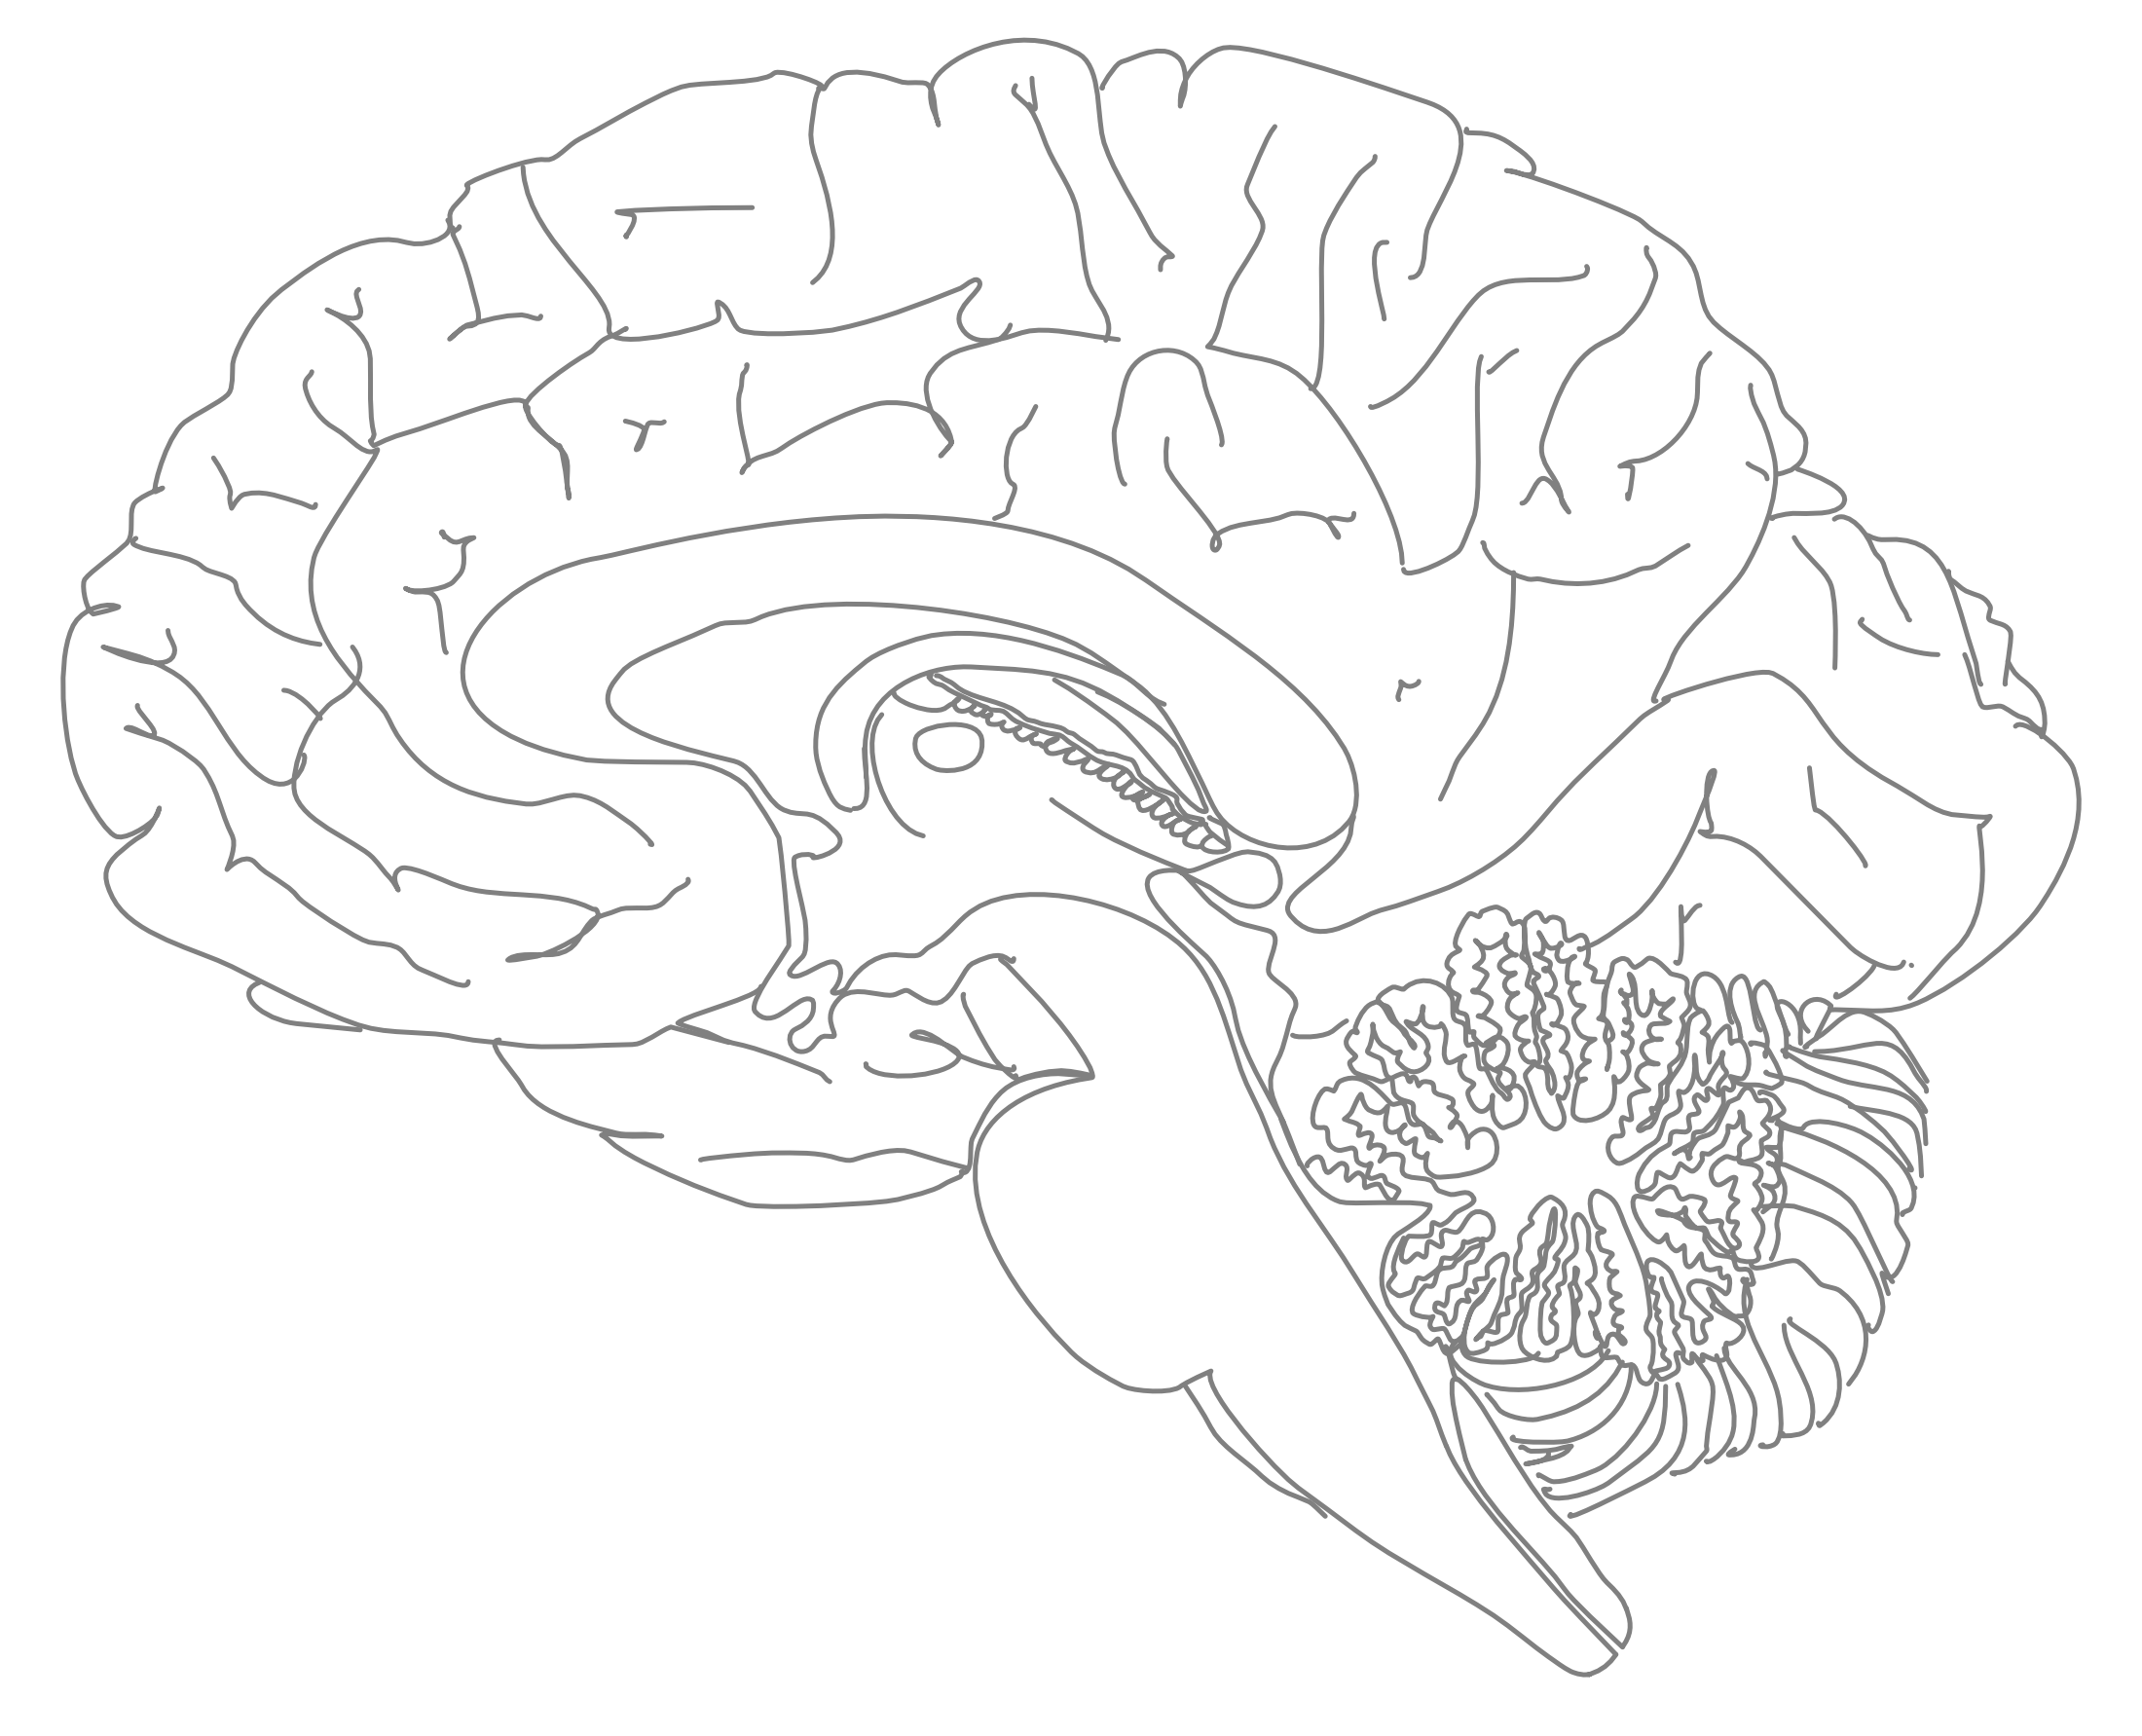
\includegraphics[width=0.7\linewidth]{./figures/cns/brain_for_labeling_medial_III} 

}

\caption{(ref:blmiii)}\label{fig:bflmiii}
\end{figure}

\hypertarget{cytoarchitectonic-areas-according-to-brodmann}{%
\section{Cytoarchitectonic Areas According To Brodmann}\label{cytoarchitectonic-areas-according-to-brodmann}}

\begin{enumerate}
\def\labelenumi{\arabic{enumi}.}
\tightlist
\item
  Label the highlighted areas with the corresponding numbers given by Broadmann.
\end{enumerate}



\begin{figure}

{\centering 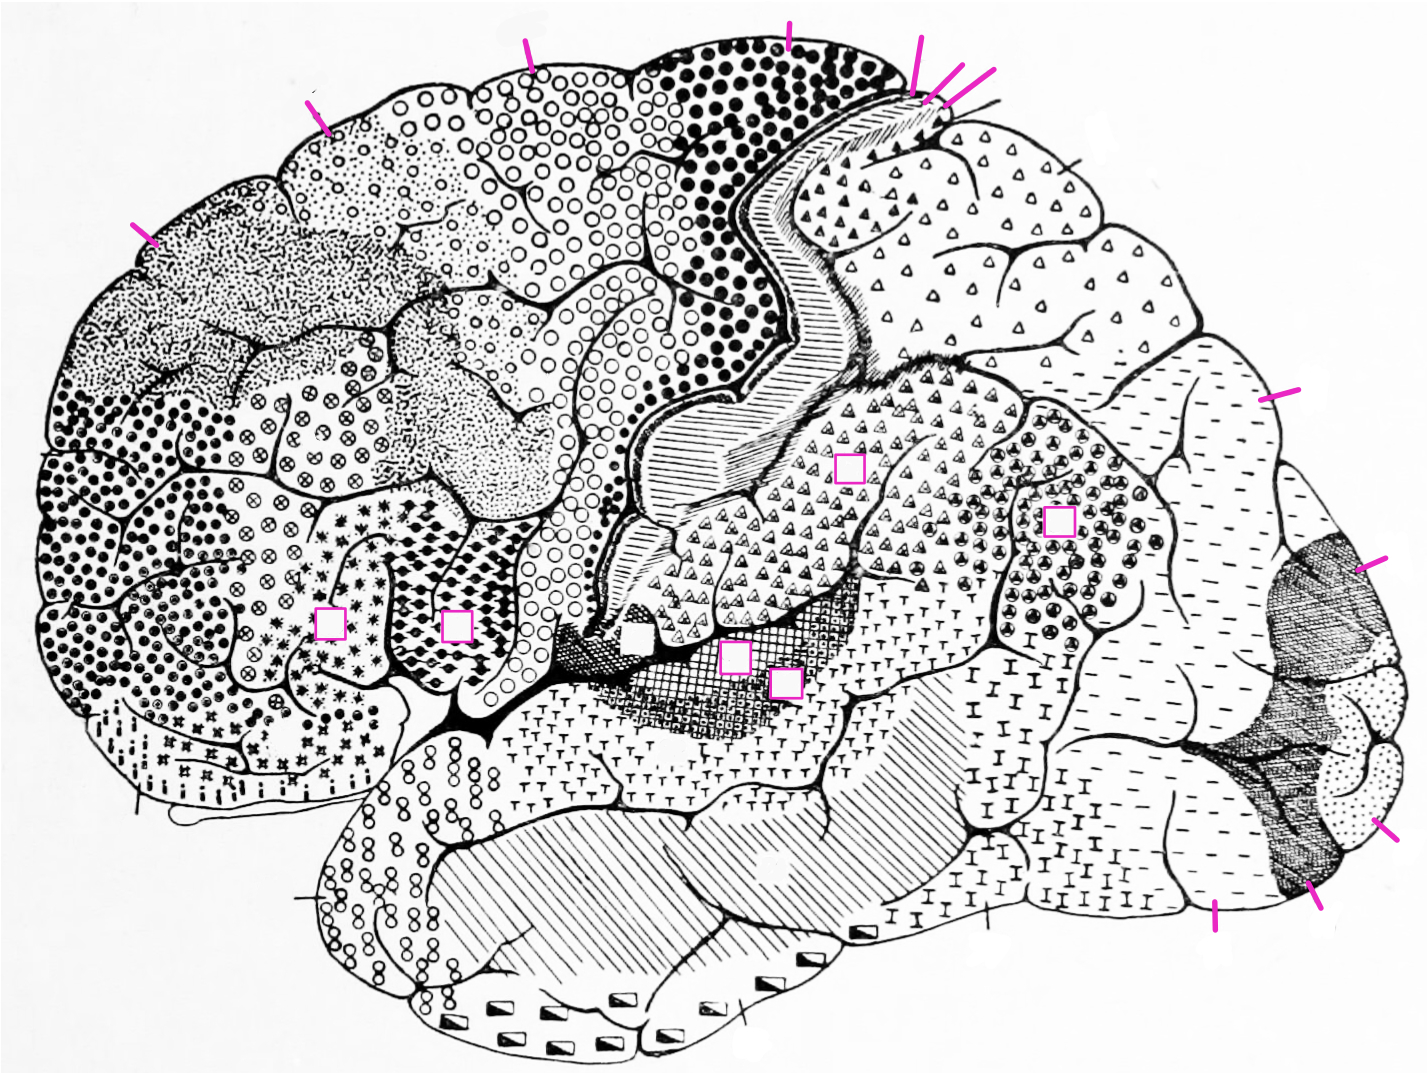
\includegraphics[width=0.7\linewidth]{./figures/cns/Brodmann_lateral} 

}

\caption{A lateral view of the cytoarchitectonic areas of the human brain according to Brodmann.}\label{fig:brodl}
\end{figure}

\begin{enumerate}
\def\labelenumi{\arabic{enumi}.}
\tightlist
\item
  Label the highlighted Brodamann areas with the corresponding numbers.
  A medial view of the cytoarchitectonic areas of the human brain according to Brodmann. A medial view of the cytoarchitectonic areas of the human brain according to Brodmann
\end{enumerate}



\begin{figure}

{\centering 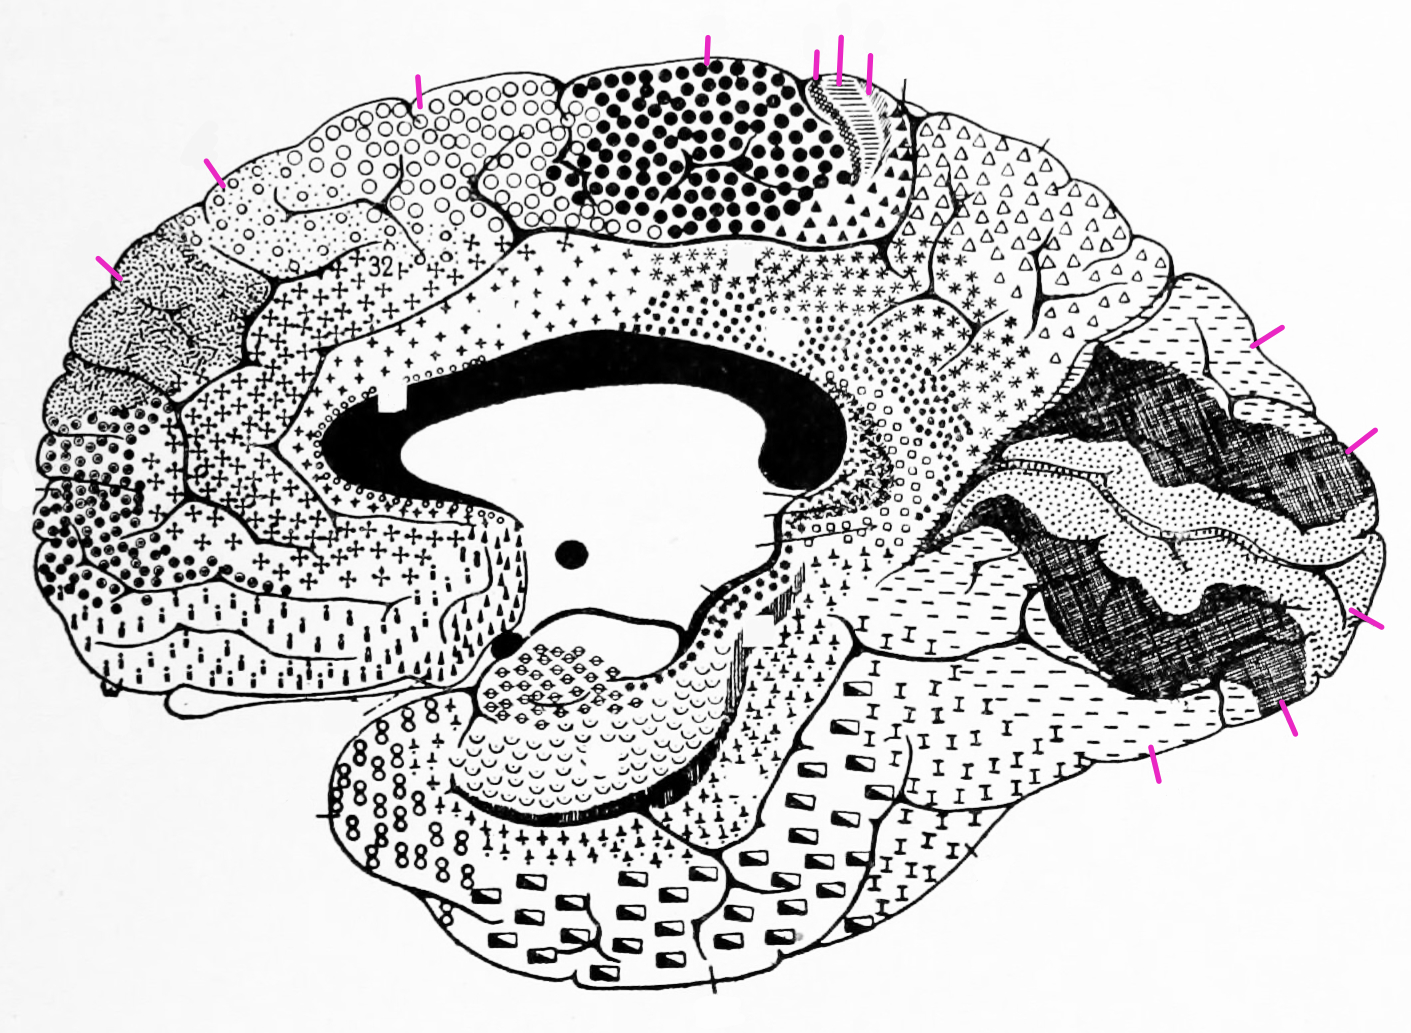
\includegraphics[width=0.7\linewidth]{./figures/cns/Brodmann_medial} 

}

\caption{A medial view of the cytoarchitectonic areas of the human brain according to Brodmann.}\label{fig:brodm}
\end{figure}

\hypertarget{the-telencephalon}{%
\chapter{The Telencephalon}\label{the-telencephalon}}

In this laboratory session, we will study the anatomy of the human telencephalon. The cerebrum or telencephalon is a large part of the brain containing the cerebral cortex (of the two cerebral hemispheres), as well as several subcortical structures, including the hippocampus, basal ganglia, and olfactory bulb. In the human brain, the cerebrum is the uppermost region of the central nervous system. The prosencephalon or forebrain is the embryonic structure from which the cerebrum develops prenatally. In mammals, the dorsal telencephalon, or pallium, develops into the cerebral cortex, and the ventral telencephalon, or subpallium, becomes the basal ganglia. The cerebrum is also divided into approximately symmetric left and right cerebral hemispheres.

Below, you will be presented with a number of figures and asked to label or color certain structures in each figure.

\hypertarget{a-series-of-coronal-sections-of-a-human-brain}{%
\section{A Series Of Coronal Sections Of A Human Brain}\label{a-series-of-coronal-sections-of-a-human-brain}}

In Figure \ref{fig:1520}, label the following structures:

\begin{enumerate}
\def\labelenumi{\arabic{enumi}.}
\tightlist
\item
  The cingulate sulcus
\item
  The cingulate gyrus
\item
  The corpus callosum
\item
  The lateral ventricle
\item
  The caudate nucleus
\item
  The insula
\item
  The lateral sulcus
\item
  The superior temporal gyrus
\item
  The superior temporal sulcus
\item
  The middle temporal gyrus
\item
  The middle temporal sulcus
\item
  The inferior temporal gyrus
\item
  The inferior temporal sulcus
\item
  The putamen
\item
  The nucleus accumbens
\item
  The optic nerves (left and right)
\item
  The septum pelucidum
\item
  The septal nuclei
\item
  The internal capsule
\item
  The external capsule
\item
  The entorhinal cortex
\item
  The parahippocampal gyrus
\end{enumerate}



\begin{figure}

{\centering 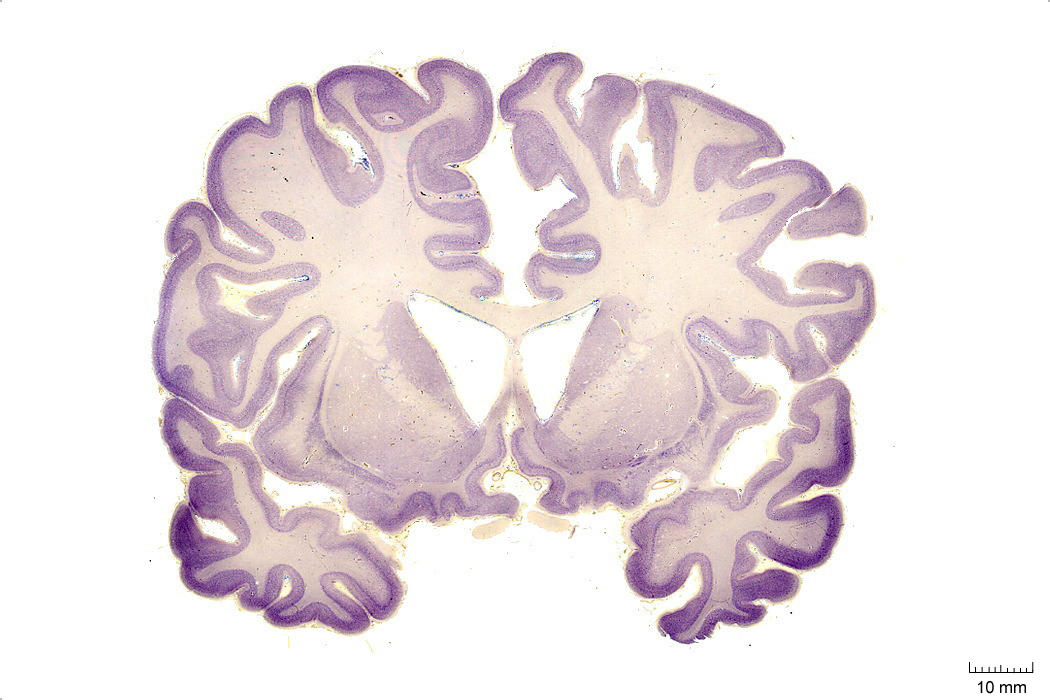
\includegraphics[width=0.7\linewidth]{./figures/cns/1520_cell} 

}

\caption{Coronal section from \href{https://msu.edu/~brains/brains/human/index.html}{The Human Brain Atlas} at the \href{https://msu.edu/~brains/copyright.html}{Michigan State University Brain Biodiveristy Bank} which \href{https://msu.edu/~brains/copyright.html}{acknowledges} their support from the National Science Foundation.}\label{fig:1520}
\end{figure}

In Figure \ref{fig:1680}, label the following structures:

\begin{enumerate}
\def\labelenumi{\arabic{enumi}.}
\tightlist
\item
  The cingulate sulcus
\item
  The cingulate gyrus
\item
  The corpus callosum
\item
  The fornix
\item
  The lateral ventricle
\item
  The choroid plexus
\item
  The anterior commissure
\item
  The insula
\item
  The lateral sulcus
\item
  The superior temporal gyrus
\item
  The superior temporal sulcus
\item
  The middle temporal gyrus
\item
  The middle temporal sulcus
\item
  The inferior temporal gyrus
\item
  The inferior temporal sulcus
\item
  The putamen
\item
  The preoptic area
\item
  The optic chiasm
\item
  The infundibular stalk
\item
  A pigment epithelial cell with extended proces
\item
  The 3\textsuperscript{d} ventricle
\item
  The internal capsule
\item
  The external capsule
\item
  The claustrum
\item
  The globus pallidus
\item
  The anterior commissure
\item
  The amygdala
\item
  The entorhinal cortex
\item
  The parahippocampal gyrus
\end{enumerate}



\begin{figure}

{\centering 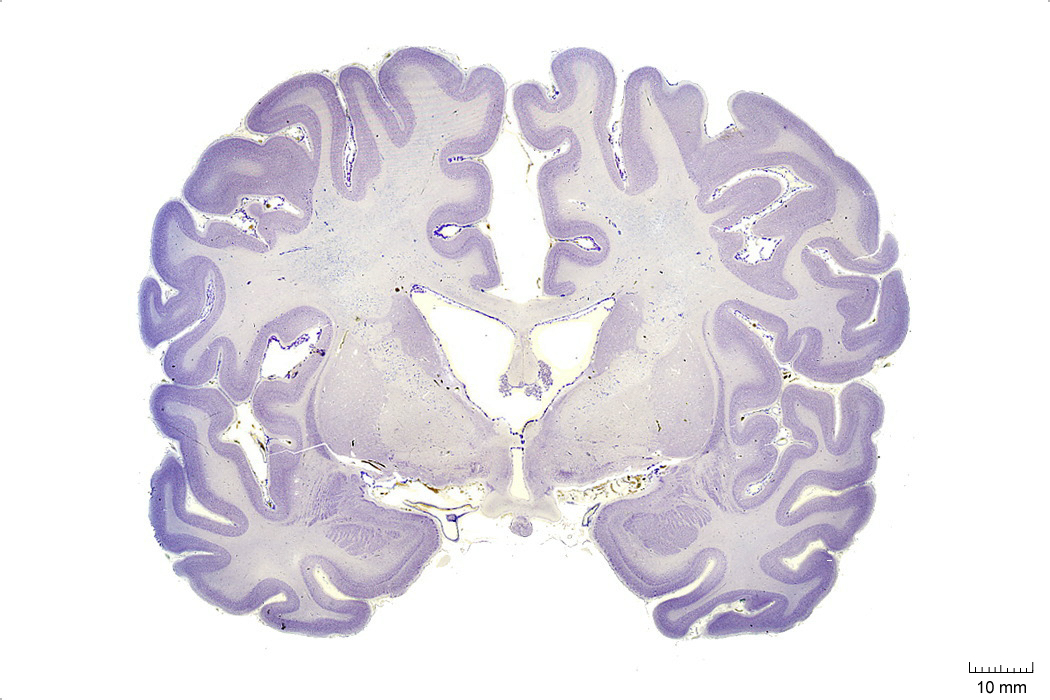
\includegraphics[width=0.7\linewidth]{./figures/cns/1680_cell} 

}

\caption{Coronal section from \href{https://msu.edu/~brains/brains/human/index.html}{The Human Brain Atlas} at the \href{https://msu.edu/~brains/copyright.html}{Michigan State University Brain Biodiveristy Bank} which \href{https://msu.edu/~brains/copyright.html}{acknowledges} their support from the National Science Foundation.}\label{fig:1680}
\end{figure}

In Figure @ref(fig:\texttt{1840}), label the following structures:

\begin{enumerate}
\def\labelenumi{\arabic{enumi}.}
\tightlist
\item
  The cingulate sulcus
\item
  The cingulate gyrus
\item
  The corpus callosum
\item
  The fornix
\item
  The lateral ventricle
\item
  The choroid plexus
\item
  The caudate nucleus
\item
  The thalamus
\item
  The insula
\item
  The lateral sulcus
\item
  The superior temporal gyrus
\item
  The superior temporal sulcus
\item
  The middle temporal gyrus
\item
  The middle temporal sulcus
\item
  The inferior temporal gyrus
\item
  The inferior temporal sulcus
\item
  The putamen
\item
  The hippocampus
\item
  The 3\textsuperscript{d} ventricle
\item
  The internal capsule
\item
  The external capsule
\item
  The claustrum
\item
  The globus pallidus
\item
  The fornix
\item
  The optic tract
\item
  The hypothalamus
\item
  The lateral ventricle
\item
  The entorhinal cortex
\item
  The parahippocampal gyrus
\item
  The amygdaloid nuclei:

  \begin{itemize}
  \tightlist
  \item
    medial
  \item
    central
  \item
    cortical
  \item
    basomedial
  \item
    basolateral
  \item
    lateral
  \end{itemize}
\end{enumerate}



\begin{figure}

{\centering 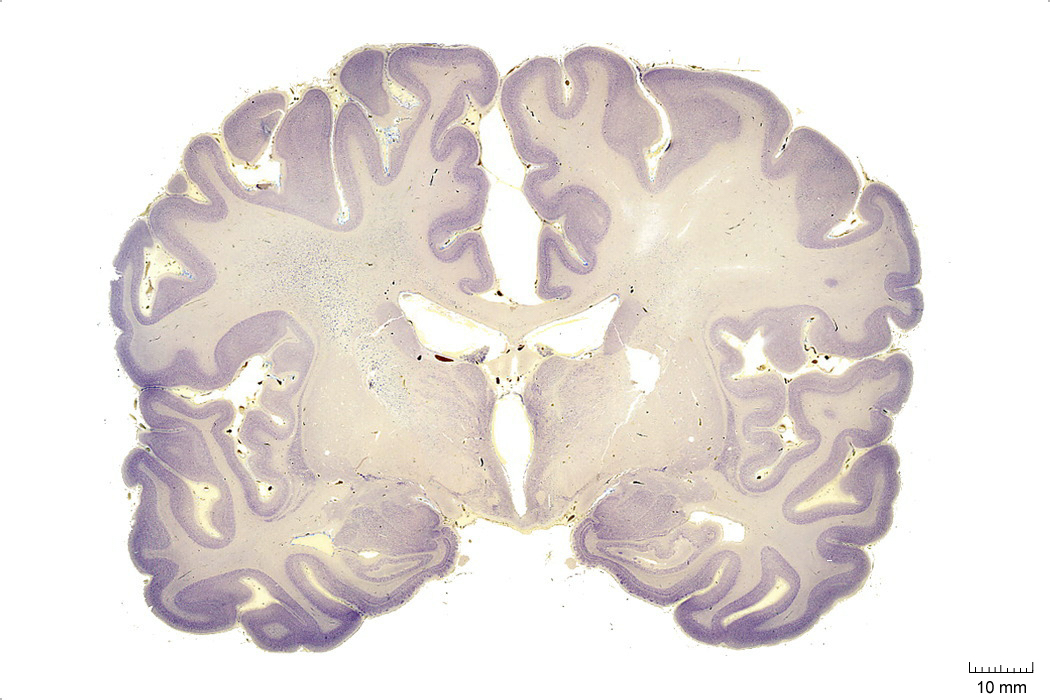
\includegraphics[width=0.7\linewidth]{./figures/cns/1840_cell} 

}

\caption{Coronal section from \href{https://msu.edu/~brains/brains/human/index.html}{The Human Brain Atlas} at the \href{https://msu.edu/~brains/copyright.html}{Michigan State University Brain Biodiveristy Bank} which \href{https://msu.edu/~brains/copyright.html}{acknowledges} their support from the National Science Foundation.}\label{fig:1840}
\end{figure}

In Figure \ref{fig:2000}, label the following structures:



\begin{enumerate}
\def\labelenumi{\arabic{enumi}.}
\tightlist
\item
  The cingulate sulcus
\item
  The cingulate gyrus
\item
  The corpus callosum
\item
  The fornix
\item
  The lateral ventricle
\item
  The choroid plexus
\item
  The caudate nucleus
\item
  The thalamus
\item
  The insula
\item
  The lateral sulcus
\item
  The superior temporal gyrus
\item
  The superior temporal sulcus
\item
  The middle temporal gyrus
\item
  The middle temporal sulcus
\item
  The inferior temporal gyrus
\item
  The inferior temporal sulcus
\item
  The putamen
\item
  The hippocampus
\item
  The dentate gyrus
\item
  The zona incerta
\item
  The substantia nigra
\item
  The 3\textsuperscript{d} ventricle
\item
  The thalamus
\item
  The internal capsule
\item
  The external capsule
\item
  The claustrum
\item
  The globus pallidus
\item
  The optic tract
\item
  The lateral ventricle
\item
  The subthalamic nucleus
\item
  The entorhinal cortex
\item
  The parahippocampal gyrus
\item
  The cerebral peduncle
\end{enumerate}

\begin{figure}

{\centering 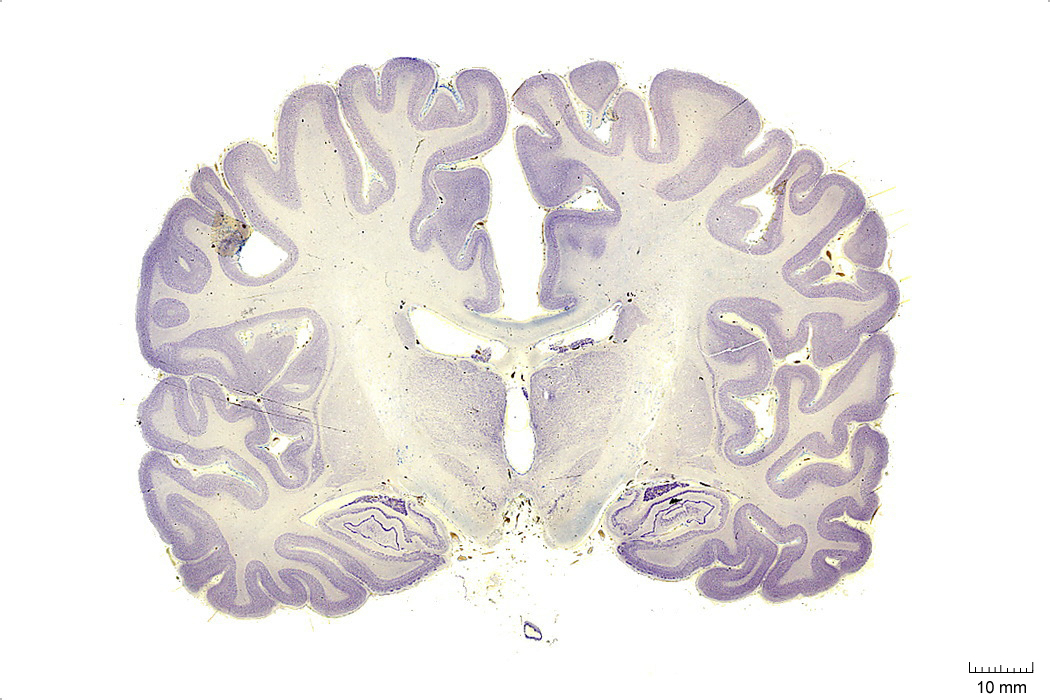
\includegraphics[width=0.7\linewidth]{./figures/cns/2000_cell} 

}

\caption{Coronal section from \href{https://msu.edu/~brains/brains/human/index.html}{The Human Brain Atlas} at the \href{https://msu.edu/~brains/copyright.html}{Michigan State University Brain Biodiveristy Bank} which \href{https://msu.edu/~brains/copyright.html}{acknowledges} their support from the National Science Foundation.}\label{fig:2000}
\end{figure}

In Figure \ref{fig:2060}, label the following structures:

\begin{enumerate}
\def\labelenumi{\arabic{enumi}.}
\tightlist
\item
  The cingulate gyrus
\item
  The corpus callosum
\item
  The fornix
\item
  The lateral ventricle
\item
  The choroid plexus
\item
  The caudate nucleus
\item
  The thalamus
\item
  The insula
\item
  The lateral sulcus
\item
  The superior temporal gyrus
\item
  The superior temporal sulcus
\item
  The middle temporal gyrus
\item
  The middle temporal sulcus
\item
  The inferior temporal gyrus
\item
  The inferior temporal sulcus
\item
  The putamen
\item
  The hippocampus
\item
  The dentate gyrus
\item
  The red nucleus
\item
  The substantia nigra
\item
  The 3\textsuperscript{d} ventricle
\item
  The thalamus
\item
  The internal capsule
\item
  The external capsule
\item
  The pons
\item
  The zona incerta
\item
  The globus pallidus
\item
  The optic tract
\item
  The lateral ventricle
\item
  The subthalamic nucleus
\item
  The entorhinal cortex
\item
  The parahippocampal gyrus
\item
  The cerebral peduncle
\end{enumerate}



\begin{figure}

{\centering 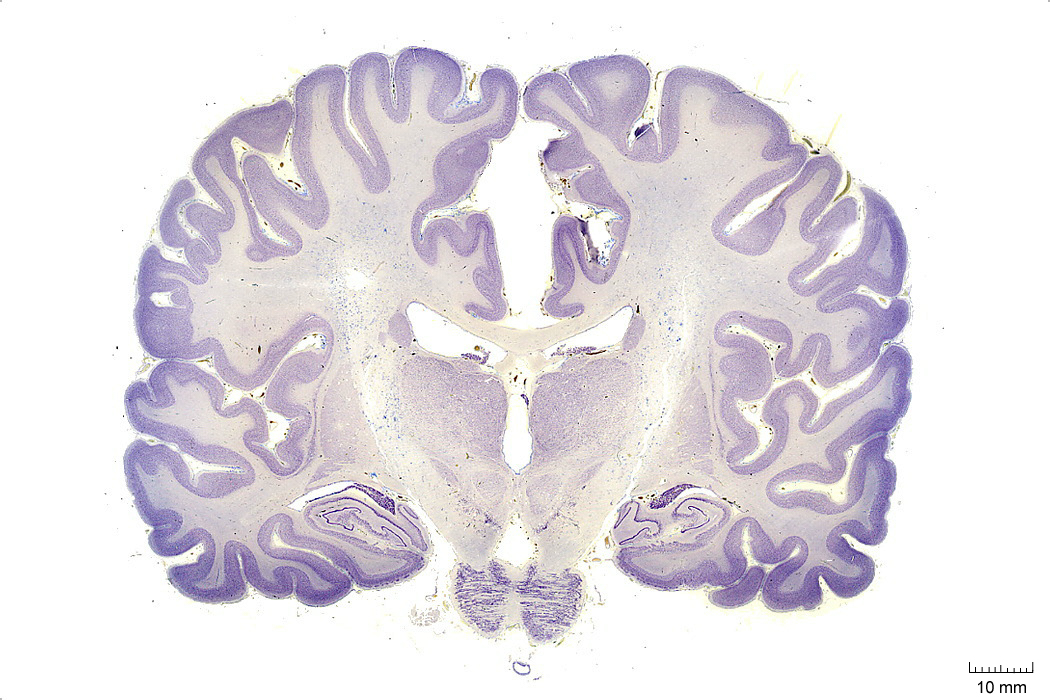
\includegraphics[width=0.7\linewidth]{./figures/cns/2060_cell} 

}

\caption{Coronal section from \href{https://msu.edu/~brains/brains/human/index.html}{The Human Brain Atlas} at the \href{https://msu.edu/~brains/copyright.html}{Michigan State University Brain Biodiveristy Bank} which \href{https://msu.edu/~brains/copyright.html}{acknowledges} their support from the National Science Foundation.}\label{fig:2060}
\end{figure}

In Figure \ref{fig:2240}, label the following structures:

\begin{enumerate}
\def\labelenumi{\arabic{enumi}.}
\tightlist
\item
  The cingulate gyrus
\item
  The corpus callosum
\item
  The fornix
\item
  The lateral ventricle
\item
  The choroid plexus
\item
  The caudate nucleus
\item
  The insula
\item
  The lateral sulcus
\item
  The superior temporal gyrus
\item
  The superior temporal sulcus
\item
  The middle temporal gyrus
\item
  The middle temporal sulcus
\item
  The inferior temporal gyrus
\item
  The inferior temporal sulcus
\item
  The putamen
\item
  The hippocampus
\item
  The dentate gyrus
\item
  The red nucleus
\item
  The substantia nigra
\item
  The decussation of the superior cerebellar peduncle
\item
  The habenula
\item
  The pineal gland
\item
  The medial geniculate nucleus
\item
  The lateral geniculate nucleus
\item
  The cerebral peduncle
\item
  The lateral ventricle
\item
  The entorhinal cortex
\item
  The parahippocampal gyrus
\item
  The posterior commissure
\item
  The cerebral aqueduct
\item
  The pons
\end{enumerate}



\begin{figure}

{\centering 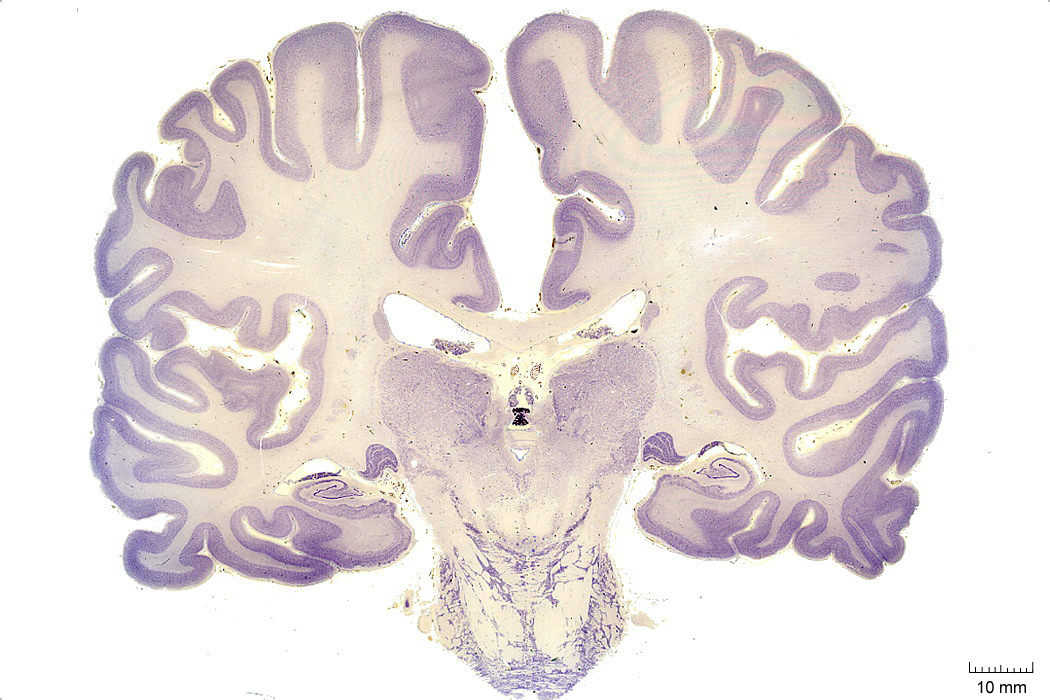
\includegraphics[width=0.7\linewidth]{./figures/cns/2240_cell} 

}

\caption{Coronal section from \href{https://msu.edu/~brains/brains/human/index.html}{The Human Brain Atlas} at the \href{https://msu.edu/~brains/copyright.html}{Michigan State University Brain Biodiveristy Bank} which \href{https://msu.edu/~brains/copyright.html}{acknowledges} their support from the National Science Foundation.}\label{fig:2240}
\end{figure}

In Figure \ref{fig:2390}, label the following structures:

\begin{enumerate}
\def\labelenumi{\arabic{enumi}.}
\tightlist
\item
  The cingulate gyrus
\item
  The corpus callosum
\item
  The fornix
\item
  The lateral ventricle
\item
  The choroid plexus
\item
  The caudate nucleus
\item
  The thalamus
\item
  The insula
\item
  The lateral sulcus
\item
  The superior temporal gyrus
\item
  The superior temporal sulcus
\item
  The middle temporal gyrus
\item
  The middle temporal sulcus
\item
  The inferior temporal gyrus
\item
  The inferior temporal sulcus
\item
  The putamen
\item
  The hippocampus
\item
  The dentate gyrus
\item
  The pineal gland
\item
  The periaqueductal grey matter
\item
  The superior cerebellar peduncle
\item
  The cerebral aqueduct
\item
  The pulvinar
\item
  The superior colliculus
\item
  The lateral ventricle
\item
  The oculomotor nucleus
\item
  The medial longitudinal fasciculus
\item
  The parahippocampal gyrus
\item
  The cerebellum
\item
  The pons
\item
  The pyramidal tract
\end{enumerate}



\begin{figure}

{\centering 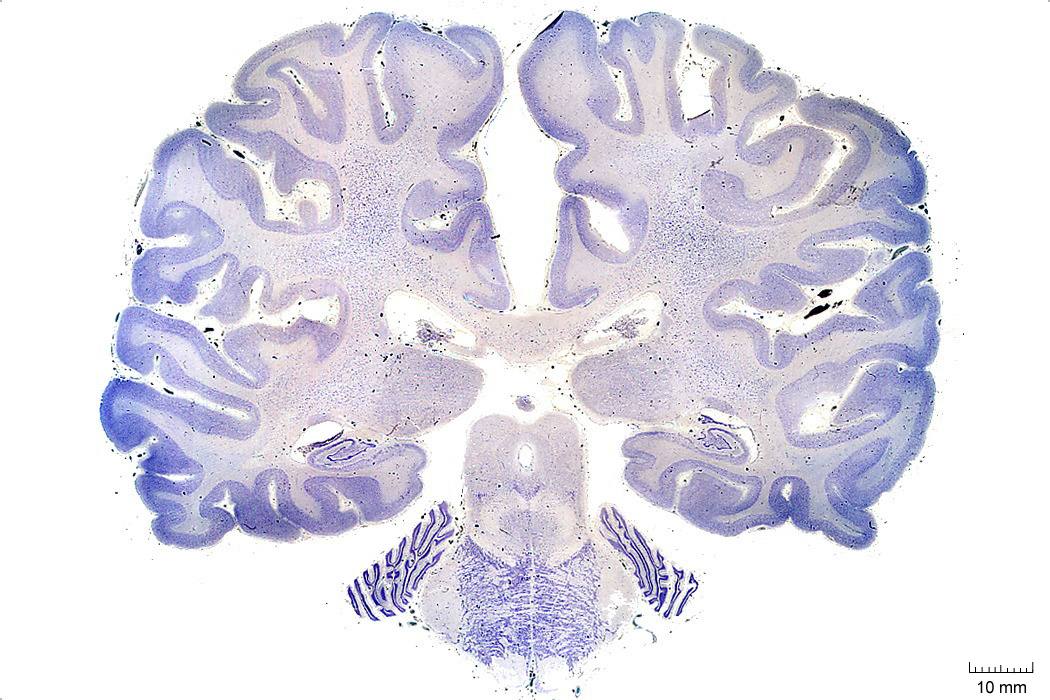
\includegraphics[width=0.7\linewidth]{./figures/cns/2390_cell} 

}

\caption{Coronal section from \href{https://msu.edu/~brains/brains/human/index.html}{The Human Brain Atlas} at the \href{https://msu.edu/~brains/copyright.html}{Michigan State University Brain Biodiveristy Bank} which \href{https://msu.edu/~brains/copyright.html}{acknowledges} their support from the National Science Foundation.}\label{fig:2390}
\end{figure}

In Figure \ref{fig:2500}, label the following structures:

\begin{enumerate}
\def\labelenumi{\arabic{enumi}.}
\tightlist
\item
  The cingulate gyrus
\item
  The corpus callosum
\item
  The fornix
\item
  The choroid plexus
\item
  The caudate nucleus
\item
  The insula
\item
  The lateral sulcus
\item
  The middle temporal gyrus
\item
  The middle temporal sulcus
\item
  The inferior temporal gyrus
\item
  The inferior temporal sulcus
\item
  The hippocampus
\item
  The dentate gyrus
\item
  The superior cerebellar peduncle
\item
  The inferior olive
\item
  The 4\textsuperscript{th} ventricle
\item
  The lateral ventricle
\item
  The inferior colliculus
\item
  The parahippocampal gyrus
\item
  The medial longitudinal fasciculus
\item
  The cerebellum
\item
  The middle cerebellar peduncle
\item
  The pontine reticular formation
\end{enumerate}



\begin{figure}

{\centering 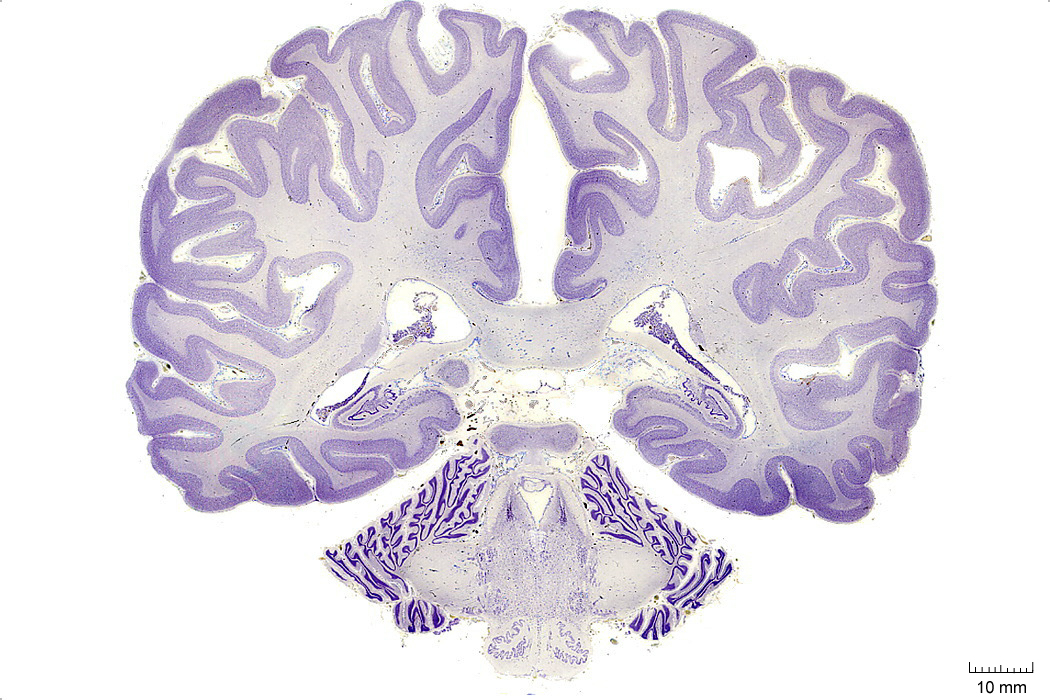
\includegraphics[width=0.7\linewidth]{./figures/cns/2500_cell} 

}

\caption{Coronal section from \href{https://msu.edu/~brains/brains/human/index.html}{The Human Brain Atlas} at the \href{https://msu.edu/~brains/copyright.html}{Michigan State University Brain Biodiveristy Bank} which \href{https://msu.edu/~brains/copyright.html}{acknowledges} their support from the National Science Foundation.}\label{fig:2500}
\end{figure}

In Figure \ref{fig:2660}, label the following structures:

\begin{enumerate}
\def\labelenumi{\arabic{enumi}.}
\tightlist
\item
  The dentate gyrus
\item
  The medial vestibular nucleus
\item
  The nucleus of the solitary tract
\item
  The solitary tract
\item
  The lateral ventricle
\item
  The 4\textsuperscript{th} ventricle
\item
  The inferior cerebellar peduncle
\item
  The inferior olive
\end{enumerate}



\begin{figure}

{\centering 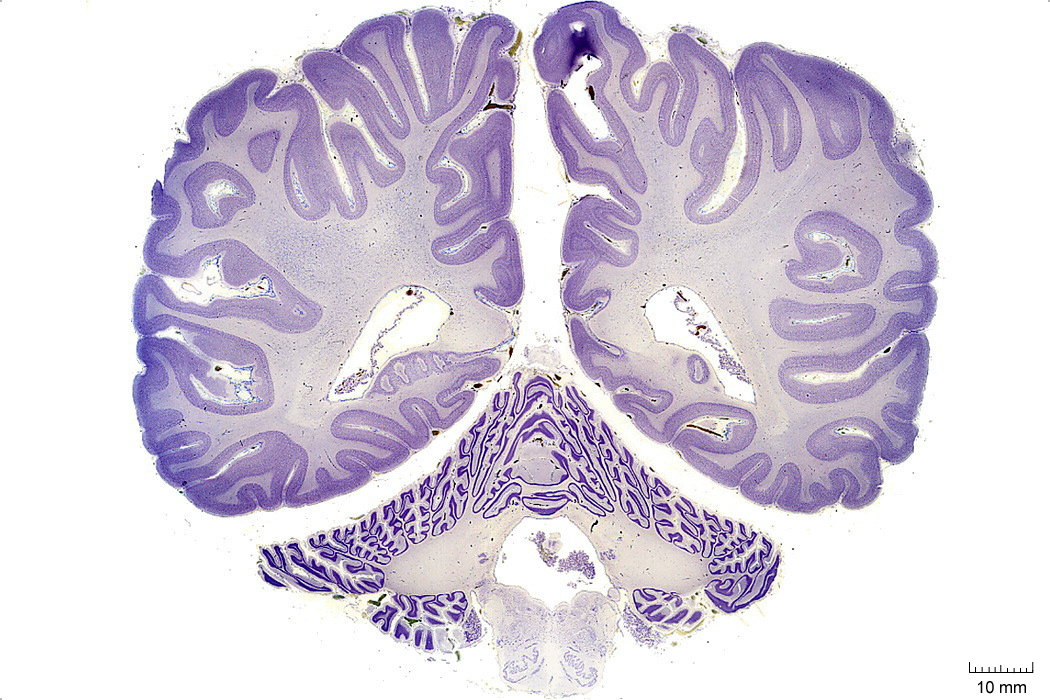
\includegraphics[width=0.7\linewidth]{./figures/cns/2660_cell} 

}

\caption{Coronal section from \href{https://msu.edu/~brains/brains/human/index.html}{The Human Brain Atlas} at the \href{https://msu.edu/~brains/copyright.html}{Michigan State University Brain Biodiveristy Bank} which \href{https://msu.edu/~brains/copyright.html}{acknowledges} their support from the National Science Foundation.}\label{fig:2660}
\end{figure}

In Figure \ref{fig:2800}, label the following structures:

\begin{enumerate}
\def\labelenumi{\arabic{enumi}.}
\tightlist
\item
  The lateral ventricle
\item
  The vermis
\item
  The cerebellum
\item
  The inferior olive
\item
  The spinal cord
\end{enumerate}



\begin{figure}

{\centering 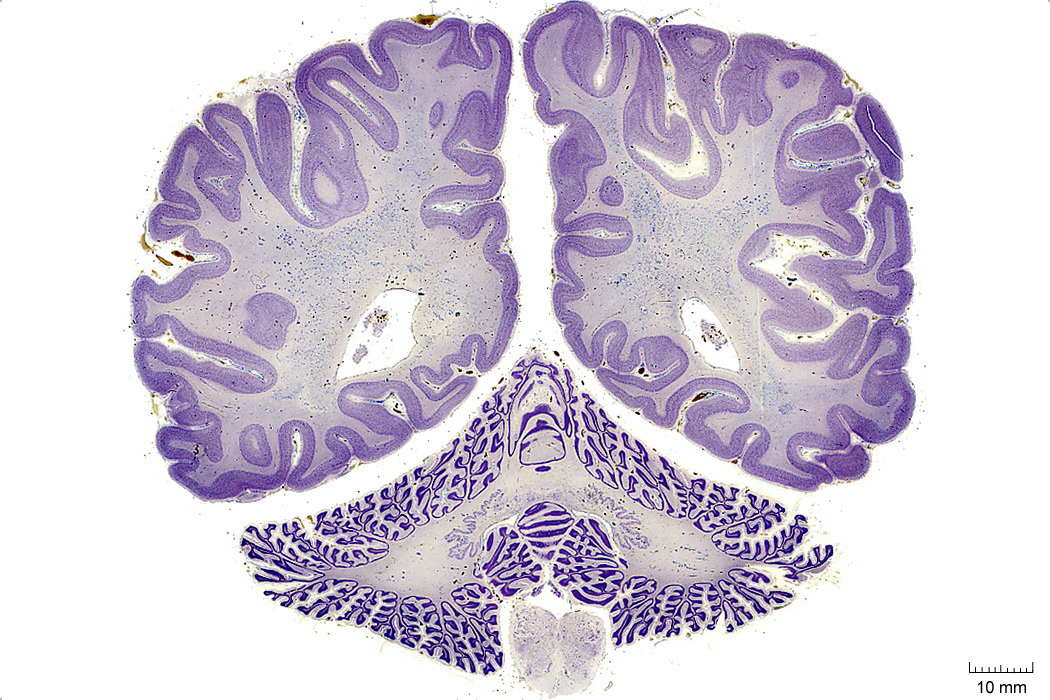
\includegraphics[width=0.7\linewidth]{./figures/cns/2800_cell} 

}

\caption{Coronal section from \href{https://msu.edu/~brains/brains/human/index.html}{The Human Brain Atlas} at the \href{https://msu.edu/~brains/copyright.html}{Michigan State University Brain Biodiveristy Bank} which \href{https://msu.edu/~brains/copyright.html}{acknowledges} their support from the National Science Foundation.}\label{fig:2800}
\end{figure}

In Figure \ref{fig:3270}, label the following structures:

\begin{enumerate}
\def\labelenumi{\arabic{enumi}.}
\tightlist
\item
  The calcarine sulcus
\item
  The striate cortex (primary visual cortex)
\item
  The vermis
\item
  The cerebellum
\item
  The spinal cord:

  \begin{itemize}
  \tightlist
  \item
    dorsal horn
  \item
    ventral horn
  \item
    dorsal column
  \item
    lateral column
  \item
    ventral column
  \end{itemize}
\end{enumerate}



\begin{figure}

{\centering 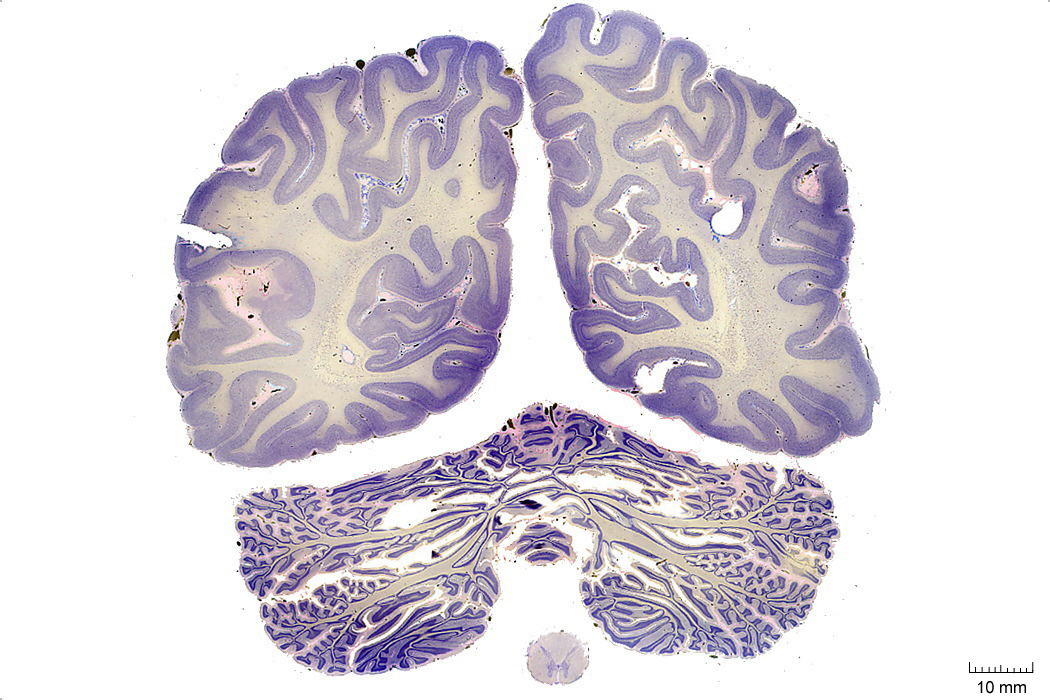
\includegraphics[width=0.7\linewidth]{./figures/cns/3270_cell} 

}

\caption{Coronal section from \href{https://msu.edu/~brains/brains/human/index.html}{The Human Brain Atlas} at the \href{https://msu.edu/~brains/copyright.html}{Michigan State University Brain Biodiveristy Bank} which \href{https://msu.edu/~brains/copyright.html}{acknowledges} their support from the National Science Foundation.}\label{fig:3270}
\end{figure}

\hypertarget{a-series-of-sagittal-sections-of-a-human-brain}{%
\section{A Series Of Sagittal Sections Of A Human Brain}\label{a-series-of-sagittal-sections-of-a-human-brain}}

In Figure \ref{fig:1492}, label the following structures:

\begin{enumerate}
\def\labelenumi{\arabic{enumi}.}
\tightlist
\item
  The lateral sulcus
\item
  The superior temporal sulcus
\item
  The middle temporal sulcus
\end{enumerate}



\begin{figure}

{\centering 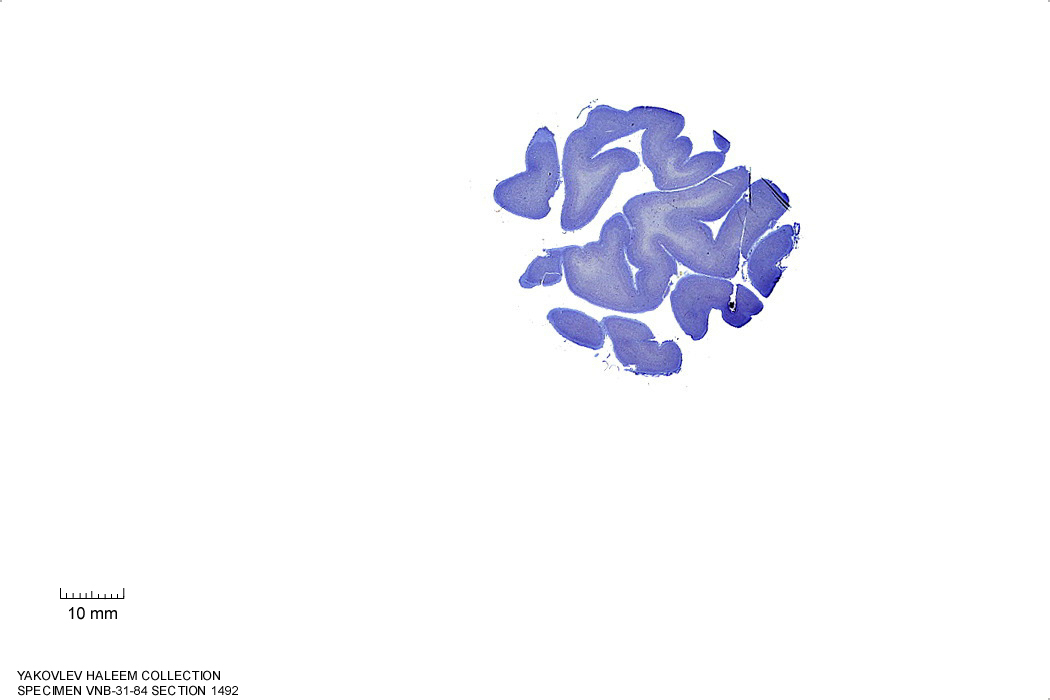
\includegraphics[width=0.7\linewidth]{./figures/cns/1492_cell} 

}

\caption{Sagittal section from \href{https://msu.edu/~brains/brains/human/index.html}{The Human Brain Atlas} at the \href{https://msu.edu/~brains/copyright.html}{Michigan State University Brain Biodiveristy Bank} which \href{https://msu.edu/~brains/copyright.html}{acknowledges} their support from the National Science Foundation.}\label{fig:1492}
\end{figure}

In Figure \ref{fig:1392}, label the following structures:

\begin{enumerate}
\def\labelenumi{\arabic{enumi}.}
\tightlist
\item
  The lateral sulcus
\item
  The superior temporal gyrus
\item
  The superior temporal sulcus
\item
  The middle temporal sulcus
\item
  The inferior temporal sulcus
\item
  The inferior temporal gyrus
\item
  The central sulcus
\item
  The precentral gyrus
\item
  The postcentral gyrus
\end{enumerate}



\begin{figure}

{\centering 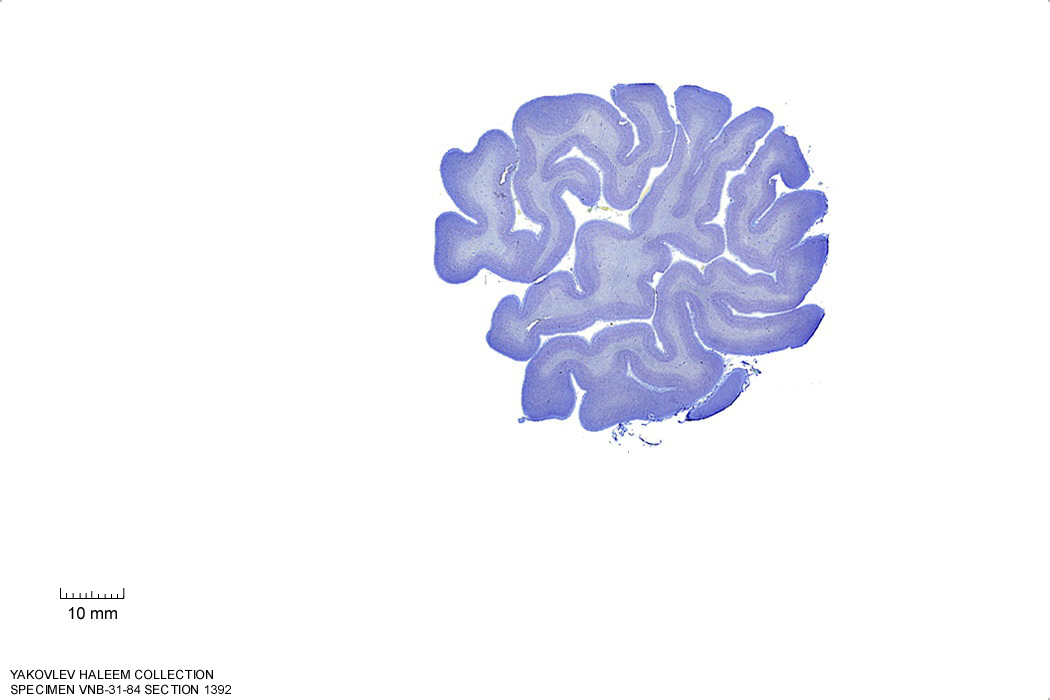
\includegraphics[width=0.7\linewidth]{./figures/cns/1392_cell} 

}

\caption{Sagittal section from \href{https://msu.edu/~brains/brains/human/index.html}{The Human Brain Atlas} at the \href{https://msu.edu/~brains/copyright.html}{Michigan State University Brain Biodiveristy Bank} which \href{https://msu.edu/~brains/copyright.html}{acknowledges} their support from the National Science Foundation.}\label{fig:1392}
\end{figure}

In Figure \ref{fig:1232}, label the following structures:

\begin{enumerate}
\def\labelenumi{\arabic{enumi}.}
\tightlist
\item
  The middle frontal gyrus
\item
  The inferior frontal sulcus
\item
  The inferior frontal gyrus
\end{enumerate}

\begin{itemize}
\tightlist
\item
  oprecular part
\item
  triangular part
\item
  orbital part
\end{itemize}

\begin{enumerate}
\def\labelenumi{\arabic{enumi}.}
\tightlist
\item
  The lateral sulcus
\item
  The superior temporal gyrus
\item
  The superior temporal sulcus
\item
  The middle temporal sulcus
\item
  The inferior temporal sulcus
\item
  The inferior temporal gyrus
\item
  The precentral sulcus
\item
  The precentral gyrus
\item
  The central sulcus
\item
  The postcentral gyrus
\item
  The postcentral sulcus
\item
  The transverse tremporal sulci
\item
  Heschl's gyrus
\end{enumerate}



\begin{figure}

{\centering 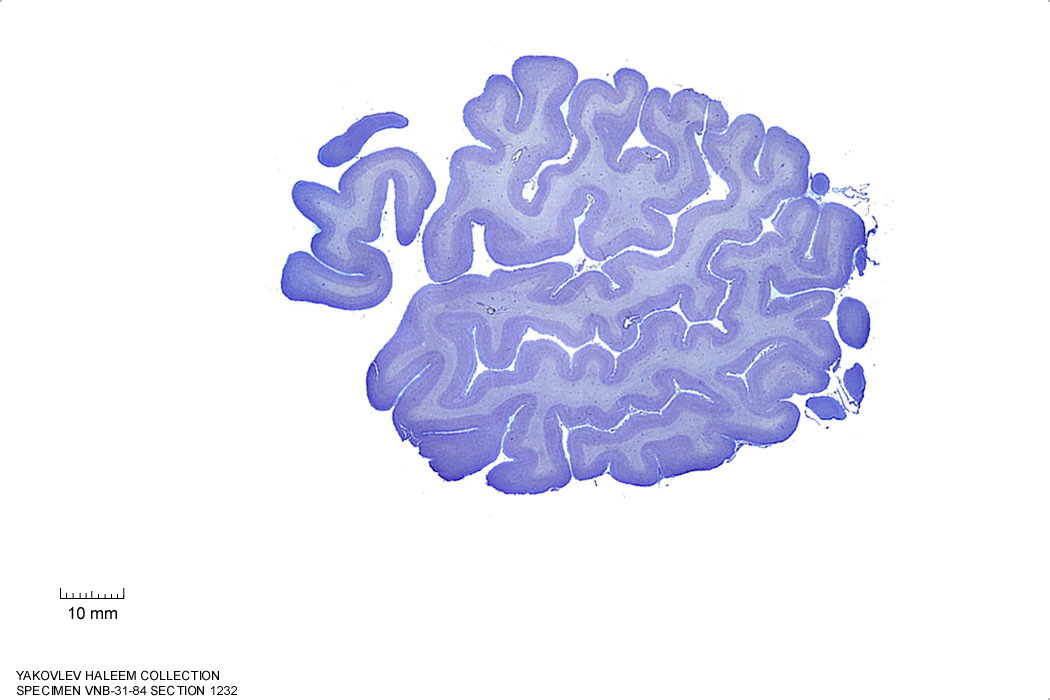
\includegraphics[width=0.7\linewidth]{./figures/cns/1232_cell} 

}

\caption{(ref:s1232)}\label{fig:1232}
\end{figure}

In Figure \ref{fig:1022}, label the following structures:

\begin{enumerate}
\def\labelenumi{\arabic{enumi}.}
\tightlist
\item
  The insula
\item
  The lateral sulcus
\item
  The cerebellum
\end{enumerate}



\begin{figure}

{\centering 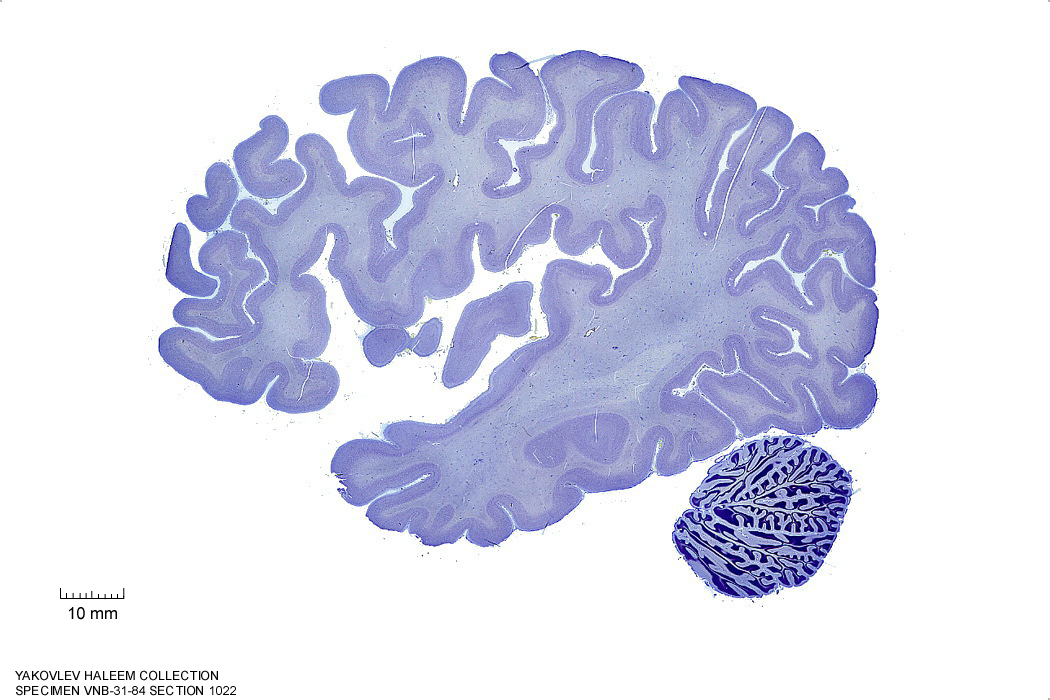
\includegraphics[width=0.7\linewidth]{./figures/cns/1022_cell} 

}

\caption{Sagittal section from \href{https://msu.edu/~brains/brains/human/index.html}{The Human Brain Atlas} at the \href{https://msu.edu/~brains/copyright.html}{Michigan State University Brain Biodiveristy Bank} which \href{https://msu.edu/~brains/copyright.html}{acknowledges} their support from the National Science Foundation.}\label{fig:1022}
\end{figure}

In Figure \ref{fig:902}, label the following structures:

\begin{enumerate}
\def\labelenumi{\arabic{enumi}.}
\tightlist
\item
  The insula
\item
  The claustrum
\item
  The tail of the caudate nucleus
\item
  The hippocampus
\item
  The lateral ventricle
\item
  The cerebellum
\end{enumerate}



\begin{figure}

{\centering 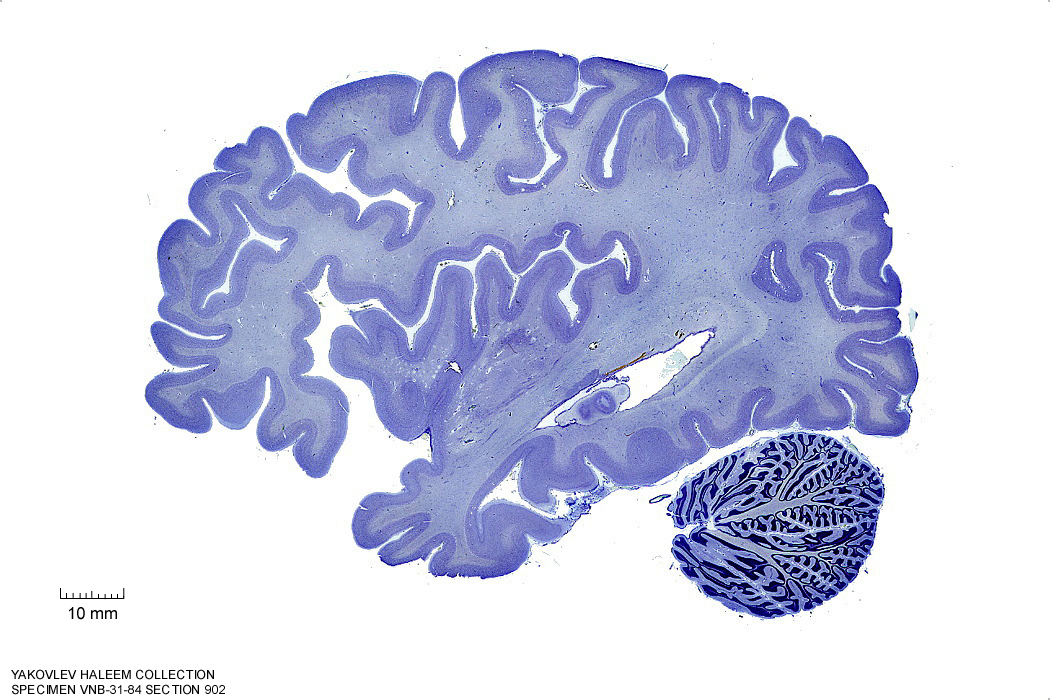
\includegraphics[width=0.7\linewidth]{./figures/cns/0902_cell} 

}

\caption{Sagittal section from \href{https://msu.edu/~brains/brains/human/index.html}{The Human Brain Atlas} at the \href{https://msu.edu/~brains/copyright.html}{Michigan State University Brain Biodiveristy Bank} which \href{https://msu.edu/~brains/copyright.html}{acknowledges} their support from the National Science Foundation.}\label{fig:902}
\end{figure}

In Figure \ref{fig:842}, label the following structures:

\begin{enumerate}
\def\labelenumi{\arabic{enumi}.}
\tightlist
\item
  The external capsule
\item
  The internal capsule
\item
  The claustrum
\item
  The putamen
\item
  The anterior commissure
\item
  The tail of the caudate nucleus
\item
  The hippocampus
\item
  The dentate gyrus
\item
  The cerebellum
\end{enumerate}



\begin{figure}

{\centering 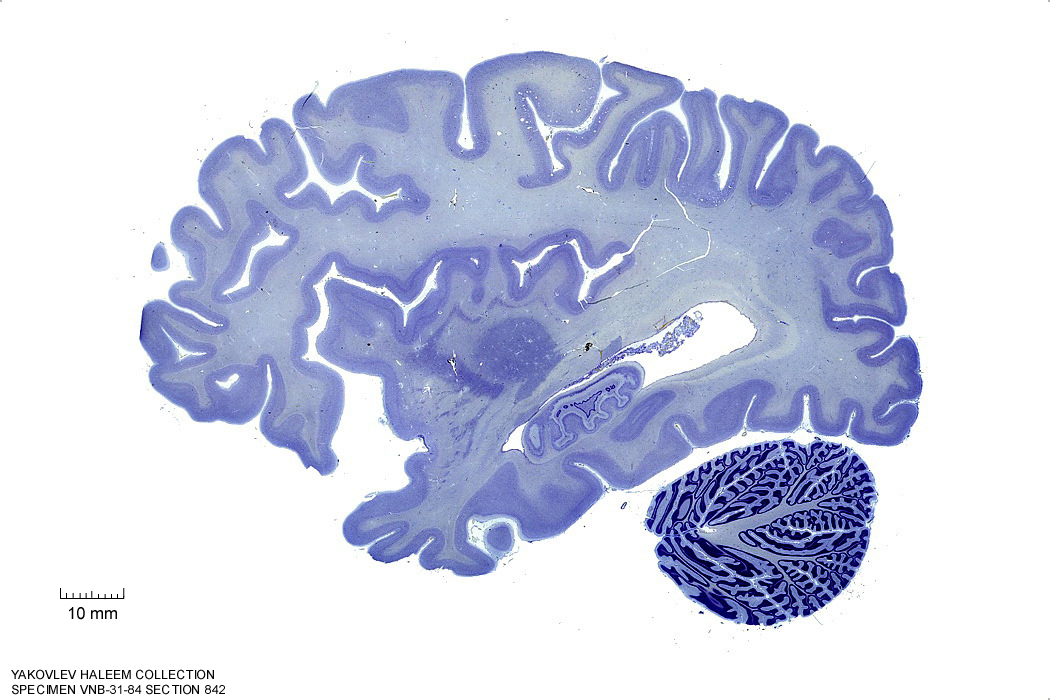
\includegraphics[width=0.7\linewidth]{./figures/cns/0842_cell} 

}

\caption{Sagittal section from \href{https://msu.edu/~brains/brains/human/index.html}{The Human Brain Atlas} at the \href{https://msu.edu/~brains/copyright.html}{Michigan State University Brain Biodiveristy Bank} which \href{https://msu.edu/~brains/copyright.html}{acknowledges} their support from the National Science Foundation.}\label{fig:842}
\end{figure}

In Figure \ref{fig:782}, label the following structures:

\begin{enumerate}
\def\labelenumi{\arabic{enumi}.}
\tightlist
\item
  The external capsule
\item
  The internal capsule
\item
  The claustrum
\item
  The putamen
\item
  The anterior commissure
\item
  The amygdala
\item
  The optic tract
\item
  The tail of the caudate nucleus
\item
  The hippocampus
\item
  The dentate gyrus
\item
  The cerebellum
\end{enumerate}



\begin{figure}

{\centering 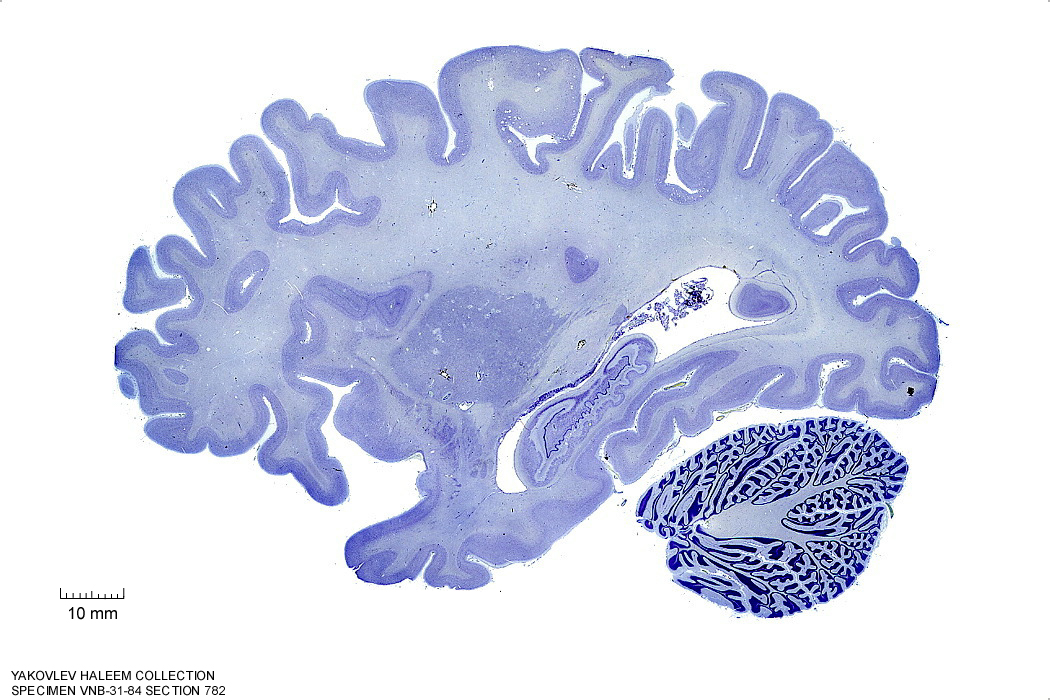
\includegraphics[width=0.7\linewidth]{./figures/cns/0782_cell} 

}

\caption{Sagittal section from \href{https://msu.edu/~brains/brains/human/index.html}{The Human Brain Atlas} at the \href{https://msu.edu/~brains/copyright.html}{Michigan State University Brain Biodiveristy Bank} which \href{https://msu.edu/~brains/copyright.html}{acknowledges} their support from the National Science Foundation.}\label{fig:782}
\end{figure}

In Figure \ref{fig:722}, label the following structures:

\begin{enumerate}
\def\labelenumi{\arabic{enumi}.}
\tightlist
\item
  The external capsule
\item
  The internal capsule
\item
  The claustrum
\item
  The putamen
\item
  The anterior commissure
\item
  The amygdala
\item
  The optic tract
\item
  The lateral geniculate nucleus
\item
  The tail of the caudate nucleus
\item
  The hippocampus
\item
  The dentate gyrus
\item
  The cerebellum
\end{enumerate}



\begin{figure}

{\centering 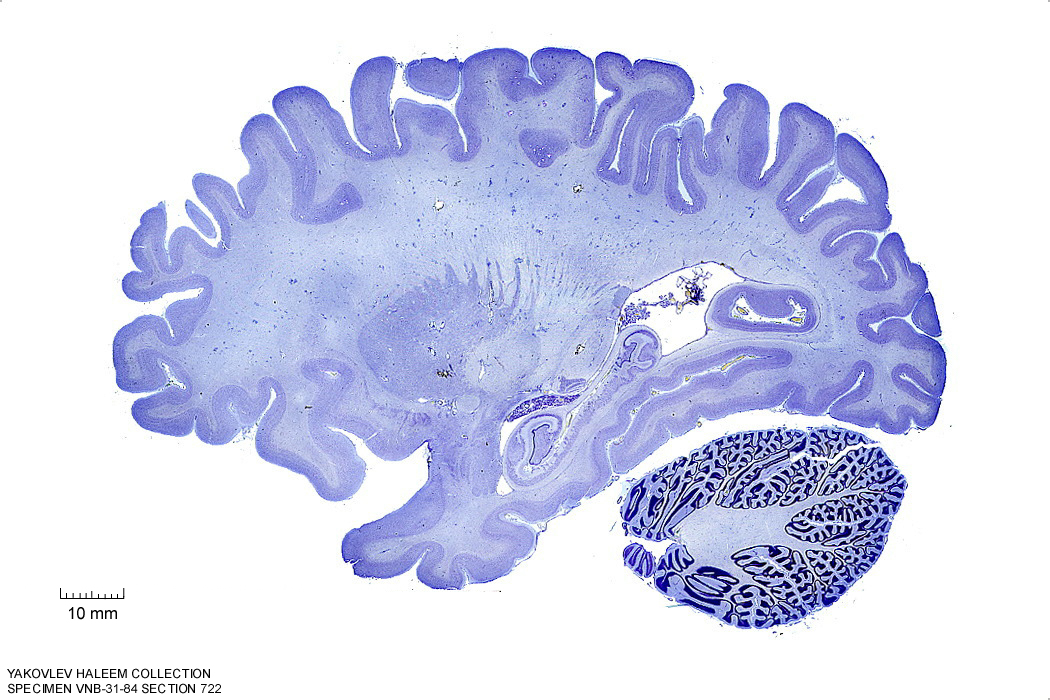
\includegraphics[width=0.7\linewidth]{./figures/cns/0722_cell} 

}

\caption{Sagittal section from \href{https://msu.edu/~brains/brains/human/index.html}{The Human Brain Atlas} at the \href{https://msu.edu/~brains/copyright.html}{Michigan State University Brain Biodiveristy Bank} which \href{https://msu.edu/~brains/copyright.html}{acknowledges} their support from the National Science Foundation.}\label{fig:722}
\end{figure}

In Figure \ref{fig:572}, label the following structures:

\begin{enumerate}
\def\labelenumi{\arabic{enumi}.}
\tightlist
\item
  The thalamic nuclei
\end{enumerate}

\begin{itemize}
\tightlist
\item
  pulvinar
\item
  ventral group
\item
  medial geniculate nucleus
\end{itemize}

\begin{enumerate}
\def\labelenumi{\arabic{enumi}.}
\tightlist
\item
  The internal capsule
\item
  The claustrum
\item
  The putamen
\item
  The anterior commissure
\item
  The amygdala
\item
  The optic tract
\item
  The lateral geniculate nucleus
\item
  The ventral pallidum
\item
  The cerebral peduncle
\item
  The superior temporal gyrus
\item
  The caudate nucleus
\item
  The hippocampus
\item
  The middle cerebellar peduncle
\item
  The cerebellum
\item
  The brachium of the superior colliculus
\item
  The corpus callosum
\item
  The fornix
\item
  The superior frontal gyrus
\item
  The lateral ventricle
\end{enumerate}



\begin{figure}

{\centering 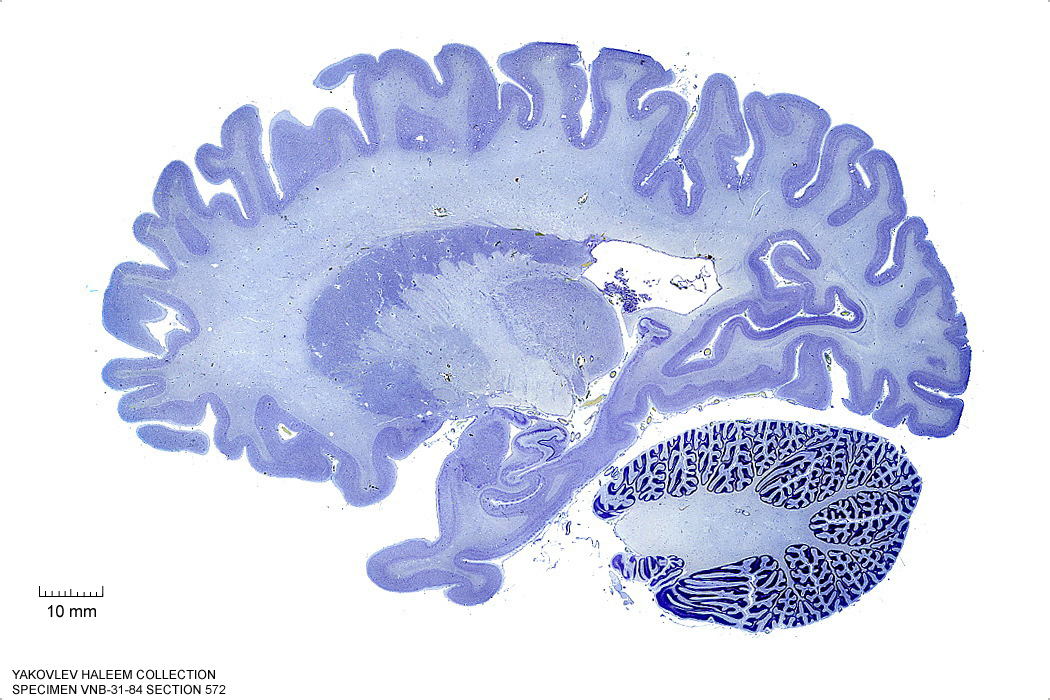
\includegraphics[width=0.7\linewidth]{./figures/cns/0572_cell} 

}

\caption{(ref:s572)}\label{fig:572}
\end{figure}

In Figure \ref{fig:512}, label the following structures:

\begin{enumerate}
\def\labelenumi{\arabic{enumi}.}
\tightlist
\item
  The thalamic nuclei
\end{enumerate}

\begin{itemize}
\tightlist
\item
  pulvinar
\item
  ventral group
\item
  medial geniculate nucleus
\end{itemize}

\begin{enumerate}
\def\labelenumi{\arabic{enumi}.}
\tightlist
\item
  The internal capsule
\item
  The globus pallidus
\item
  The ventral striatum
\item
  The anterior commissure
\item
  The amygdala
\item
  The optic tract
\item
  The lateral geniculate nucleus
\item
  The ventral pallidum
\item
  The cerebral peduncle
\item
  The superior temporal gyrus
\item
  The caudate nucleus
\item
  The hippocampus
\item
  The middle cerebellar peduncle
\item
  The cerebellum
\item
  The parieto-occipital sulcus
\item
  The brachium of the superior colliculus
\item
  The corpus callosum
\item
  The fornix
\item
  The superior frontal gyrus
\item
  The lateral ventricle
\end{enumerate}



\begin{figure}

{\centering 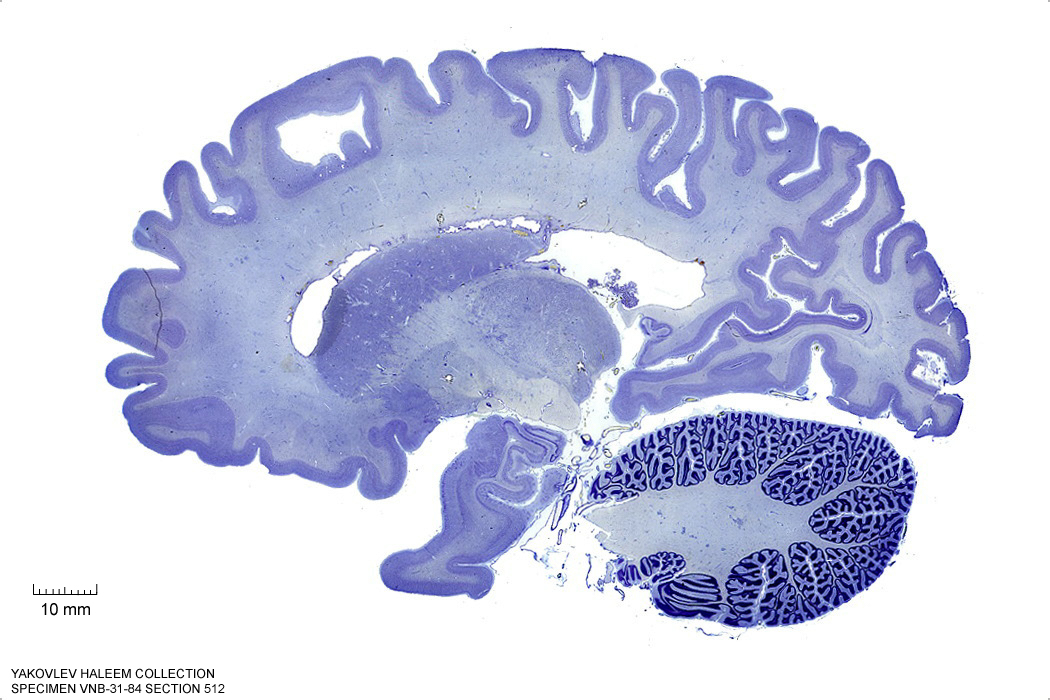
\includegraphics[width=0.7\linewidth]{./figures/cns/0512_cell} 

}

\caption{Sagittal section from \href{https://msu.edu/~brains/brains/human/index.html}{The Human Brain Atlas} at the \href{https://msu.edu/~brains/copyright.html}{Michigan State University Brain Biodiveristy Bank} which \href{https://msu.edu/~brains/copyright.html}{acknowledges} their support from the National Science Foundation.}\label{fig:512}
\end{figure}

In Figure \ref{fig:452}, label the following structures:

\begin{enumerate}
\def\labelenumi{\arabic{enumi}.}
\tightlist
\item
  The superior frontal gyrus
\item
  The thalamic nuclei
\end{enumerate}

\begin{itemize}
\tightlist
\item
  pulvinar
\end{itemize}

\begin{enumerate}
\def\labelenumi{\arabic{enumi}.}
\tightlist
\item
  The globus pallidus
\item
  The ventral striatum
\item
  The anterior commissure
\item
  The medial geniculate nucleus
\item
  The optic tract
\item
  The lateral geniculate nucleus
\item
  The ventral pallidum
\item
  The middle cerebellar peduncle
\item
  The substantia nigra
\item
  The cerebral peduncle
\item
  The subthalamic nucleus
\item
  The cerebellum
\item
  The parieto-occipital sulcus
\item
  The brachium of the superior colliculus
\item
  The corpus callosum
\item
  The fornix
\item
  The lateral ventricle
\item
  The dentate nucleus
\end{enumerate}



\begin{figure}

{\centering 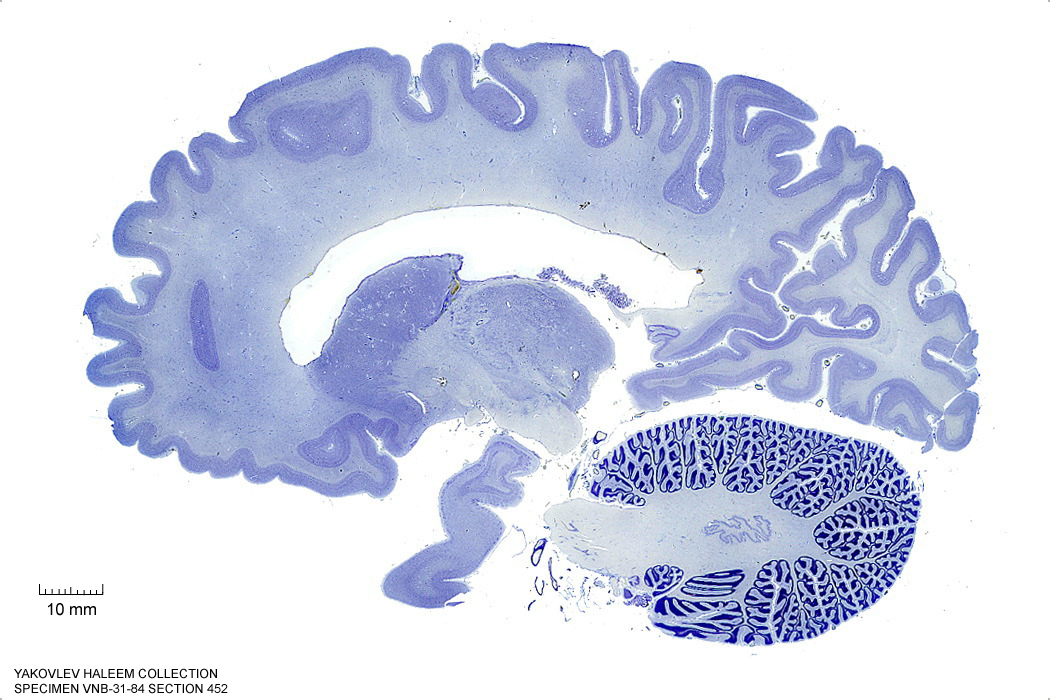
\includegraphics[width=0.7\linewidth]{./figures/cns/0452_cell} 

}

\caption{Sagittal section from \href{https://msu.edu/~brains/brains/human/index.html}{The Human Brain Atlas} at the \href{https://msu.edu/~brains/copyright.html}{Michigan State University Brain Biodiveristy Bank} which \href{https://msu.edu/~brains/copyright.html}{acknowledges} their support from the National Science Foundation.}\label{fig:452}
\end{figure}

In Figure \ref{fig:392}, label the following structures:

\begin{enumerate}
\def\labelenumi{\arabic{enumi}.}
\tightlist
\item
  The corpus callosum
\end{enumerate}

\begin{itemize}
\tightlist
\item
  the splenium
\item
  the body
\end{itemize}

\begin{enumerate}
\def\labelenumi{\arabic{enumi}.}
\tightlist
\item
  The thalamic nuclei
\end{enumerate}

\begin{itemize}
\tightlist
\item
  pulvinar
\item
  ventral group
\item
  centromedian gropup
\end{itemize}

\begin{enumerate}
\def\labelenumi{\arabic{enumi}.}
\tightlist
\item
  The anterior commissure
\item
  The optic tract
\item
  The caudate nucleus
\item
  The middle cerebellar peduncle
\item
  The cerebellum
\item
  The fornix
\item
  The superior frontal gyrus
\item
  The lateral ventricle
\item
  The parieto-occipital sulcus
\item
  The brachium of the superior colliculus
\item
  The brachium of the inferior colliculus
\item
  The dentate nucleus
\item
  The subthalamic nucleus
\end{enumerate}



\begin{figure}

{\centering 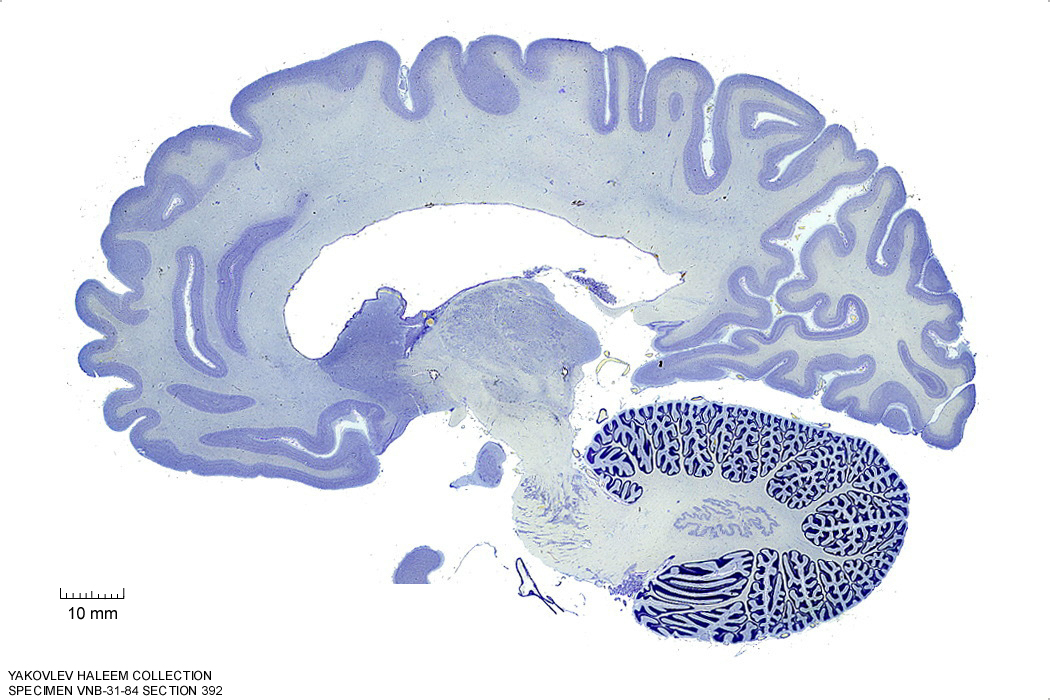
\includegraphics[width=0.7\linewidth]{./figures/cns/0392_cell} 

}

\caption{Sagittal section from \href{https://msu.edu/~brains/brains/human/index.html}{The Human Brain Atlas} at the \href{https://msu.edu/~brains/copyright.html}{Michigan State University Brain Biodiveristy Bank} which \href{https://msu.edu/~brains/copyright.html}{acknowledges} their support from the National Science Foundation.}\label{fig:392}
\end{figure}

In Figure \ref{fig:332}, label the following structures:

\begin{enumerate}
\def\labelenumi{\arabic{enumi}.}
\tightlist
\item
  The corpus callosum
\end{enumerate}

\begin{itemize}
\tightlist
\item
  the splenium
\item
  the body
\end{itemize}

\begin{enumerate}
\def\labelenumi{\arabic{enumi}.}
\tightlist
\item
  The thalamic nuclei
\end{enumerate}

\begin{itemize}
\tightlist
\item
  anterior group
\item
  ventral group
\item
  centromedian gropup
\end{itemize}

\begin{enumerate}
\def\labelenumi{\arabic{enumi}.}
\tightlist
\item
  The anterior commissure
\item
  The hypothalamus
\item
  The red nucleus
\item
  The substantia nigra
\item
  The cerebral peduncle
\item
  The superior colliculus
\item
  The pontine nuclei
\item
  The optic tract
\item
  The caudate nucleus
\item
  The middle cerebellar peduncle
\item
  The cerebellum
\item
  The fornix
\item
  The precuneus
\item
  The cuneus
\item
  The fornix
\item
  The lateral ventricle
\item
  The parieto-occipital sulcus
\item
  The dentate nucleus
\item
  The cerebellum
\item
  The inferior cerebellar peduncle
\end{enumerate}



\begin{figure}

{\centering 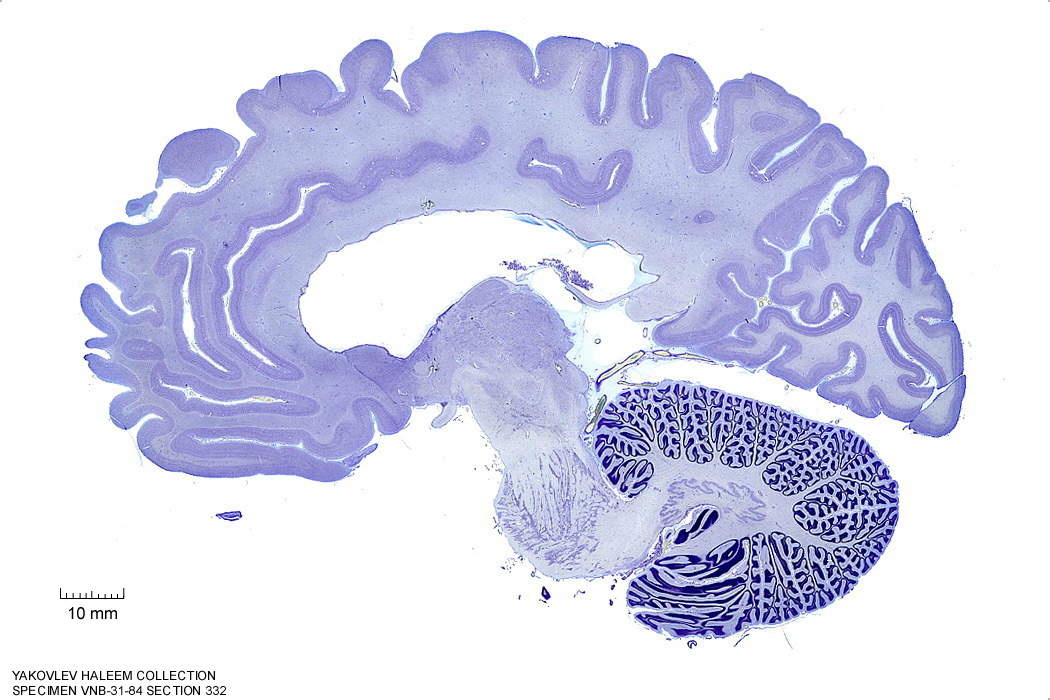
\includegraphics[width=0.7\linewidth]{./figures/cns/0332_cell} 

}

\caption{Sagittal section from \href{https://msu.edu/~brains/brains/human/index.html}{The Human Brain Atlas} at the \href{https://msu.edu/~brains/copyright.html}{Michigan State University Brain Biodiveristy Bank} which \href{https://msu.edu/~brains/copyright.html}{acknowledges} their support from the National Science Foundation.}\label{fig:332}
\end{figure}

In Figure \ref{fig:302}, label the following structures:

\begin{enumerate}
\def\labelenumi{\arabic{enumi}.}
\tightlist
\item
  The corpus callosum
\end{enumerate}

\begin{itemize}
\tightlist
\item
  the splenium
\item
  the body
\item
  the genu
\end{itemize}

\begin{enumerate}
\def\labelenumi{\arabic{enumi}.}
\tightlist
\item
  The thalamus
\item
  The anterior commissure
\item
  The mammillothalamic tract
\item
  The hypothalamus
\item
  The red nucleus
\item
  The substantia nigra
\item
  The cerebral peduncle
\item
  The superior colliculus
\item
  The inferior colliculus
\item
  The lateral lemniscus
\item
  The pontine nuclei
\item
  The inferior cerebellar peduncle
\item
  The cerebellum
\item
  The fornix
\item
  The precuneus
\item
  The cuneus
\item
  The fornix
\item
  The lateral ventricle
\item
  The parieto-occipital sulcus
\item
  The dentate nucleus
\item
  The lingual gyrus
\item
  The calcarine sulcus
\item
  The cingulate sulcus
\item
  The cingulate gyrus
\item
  The cerebellum
\end{enumerate}



\begin{figure}

{\centering 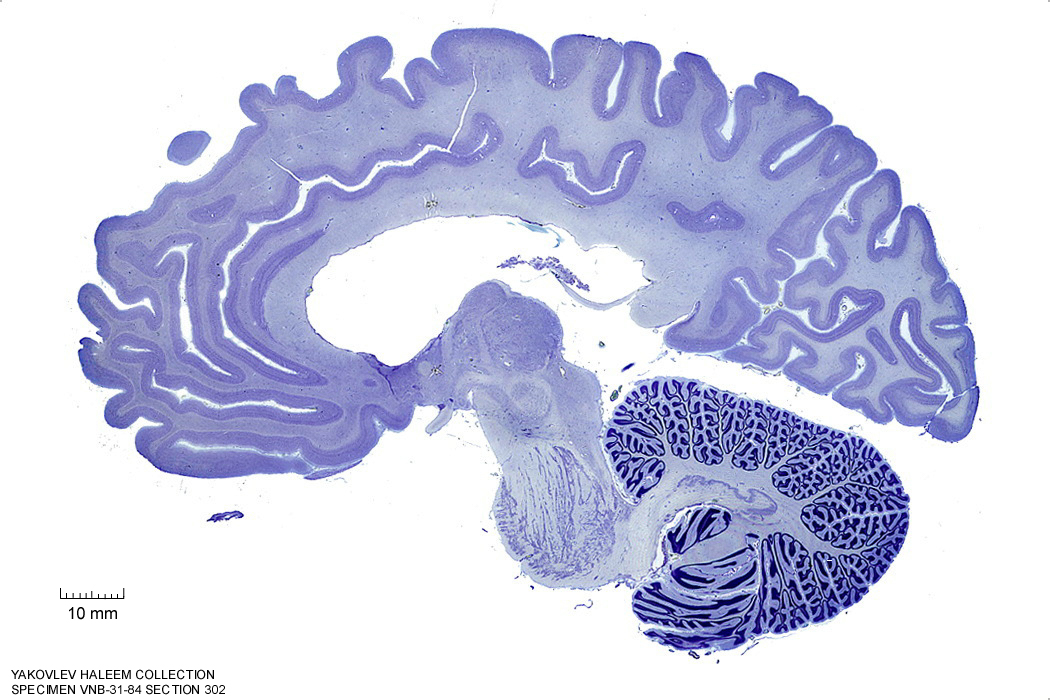
\includegraphics[width=0.7\linewidth]{./figures/cns/0302_cell} 

}

\caption{Sagittal section from \href{https://msu.edu/~brains/brains/human/index.html}{The Human Brain Atlas} at the \href{https://msu.edu/~brains/copyright.html}{Michigan State University Brain Biodiveristy Bank} which \href{https://msu.edu/~brains/copyright.html}{acknowledges} their support from the National Science Foundation.}\label{fig:302}
\end{figure}

In Figure \ref{fig:272}, label the following structures:

\begin{enumerate}
\def\labelenumi{\arabic{enumi}.}
\tightlist
\item
  The superior frontal gyrus
\item
  The corpus callosum
\end{enumerate}

\begin{itemize}
\tightlist
\item
  the splenium
\item
  the body
\item
  the genu
\end{itemize}

\begin{enumerate}
\def\labelenumi{\arabic{enumi}.}
\tightlist
\item
  The thalamus
\item
  The anterior commissure
\item
  The mammillothalamic tract
\item
  The hypothalamus
\item
  The red nucleus
\item
  The substantia nigra
\item
  The cerebral peduncle
\item
  The superior colliculus
\item
  The inferior colliculus
\item
  The lateral lemniscus
\item
  The pontine nuclei
\item
  The superior cerebellar peduncle
\item
  The inferior cerebellar peduncle
\item
  The cerebellum
\item
  The fornix
\item
  The precuneus
\item
  The cuneus
\item
  The fornix
\item
  The lateral ventricle
\item
  The parieto-occipital sulcus
\item
  The dentate nucleus
\item
  The lingual gyrus
\item
  The calcarine sulcus
\item
  The cingulate sulcus
\item
  The cingulate gyrus
\item
  The cerebellum
\end{enumerate}



\begin{figure}

{\centering 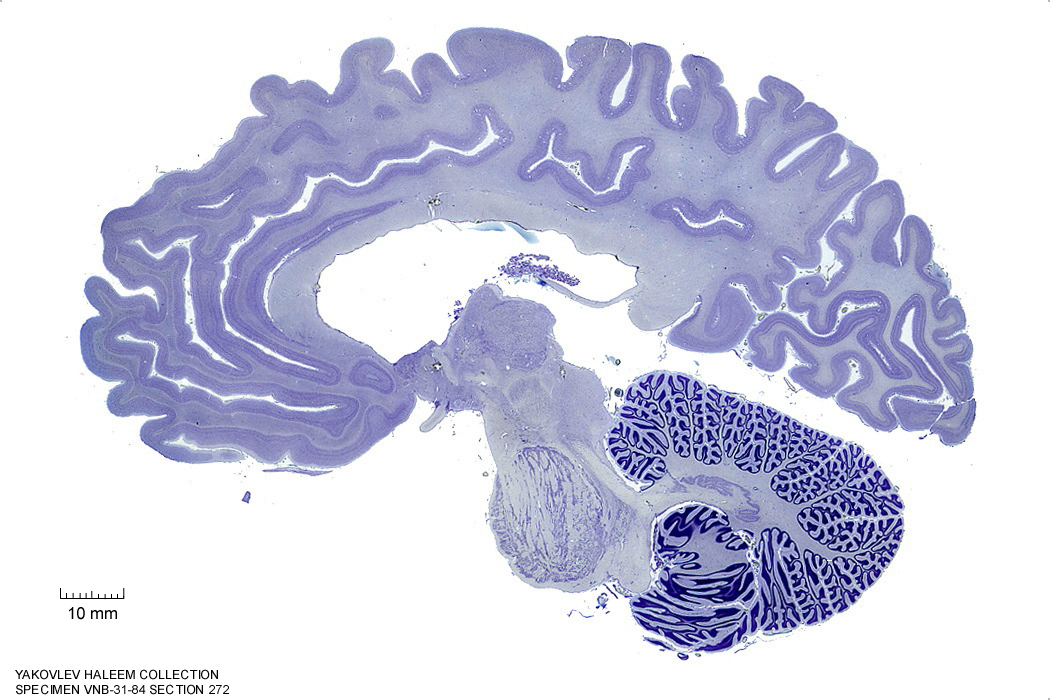
\includegraphics[width=0.7\linewidth]{./figures/cns/0272_cell} 

}

\caption{Sagittal section from \href{https://msu.edu/~brains/brains/human/index.html}{The Human Brain Atlas} at the \href{https://msu.edu/~brains/copyright.html}{Michigan State University Brain Biodiveristy Bank} which \href{https://msu.edu/~brains/copyright.html}{acknowledges} their support from the National Science Foundation.}\label{fig:272}
\end{figure}

In Figure \ref{fig:242}, label the following structures:

\begin{enumerate}
\def\labelenumi{\arabic{enumi}.}
\tightlist
\item
  The superior frontal gyrus
\item
  The corpus callosum
\end{enumerate}

\begin{itemize}
\tightlist
\item
  the splenium
\item
  the body
\item
  the genu
\end{itemize}

\begin{enumerate}
\def\labelenumi{\arabic{enumi}.}
\tightlist
\item
  The thalamus
\item
  The anterior commissure
\item
  The mammillothalamic tract
\item
  The hypothalamus
\item
  The red nucleus
\item
  The substantia nigra
\item
  The cerebral peduncle
\item
  The superior colliculus
\item
  The inferior colliculus
\item
  The lateral lemniscus
\item
  The pontine nuclei
\item
  The inferior olive
\item
  The cerebellar tonsil
\item
  The superior cerebellar peduncle
\item
  The inferior cerebellar peduncle
\item
  The cerebellum
\item
  The fornix
\item
  The precuneus
\item
  The cuneus
\item
  The fornix
\item
  The lateral ventricle
\item
  The parieto-occipital sulcus
\item
  The lingual gyrus
\item
  The calcarine sulcus
\item
  The cingulate sulcus
\item
  The cingulate gyrus
\item
  The cerebellum
\end{enumerate}



\begin{figure}

{\centering 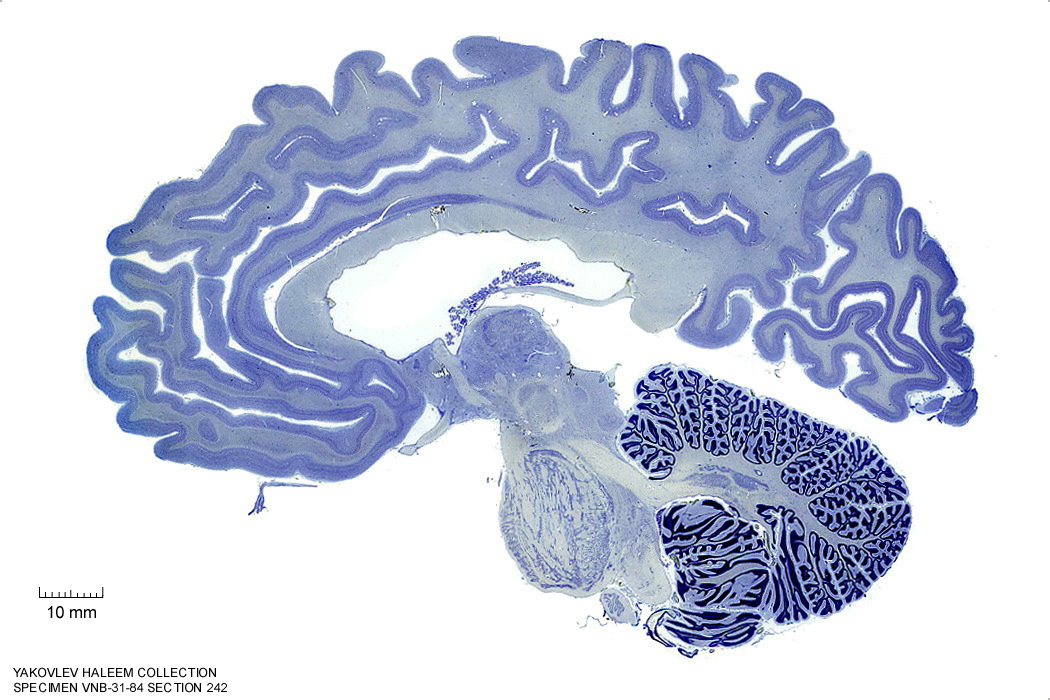
\includegraphics[width=0.7\linewidth]{./figures/cns/0242_cell} 

}

\caption{Sagittal section from \href{https://msu.edu/~brains/brains/human/index.html}{The Human Brain Atlas} at the \href{https://msu.edu/~brains/copyright.html}{Michigan State University Brain Biodiveristy Bank} which \href{https://msu.edu/~brains/copyright.html}{acknowledges} their support from the National Science Foundation.}\label{fig:242}
\end{figure}

In Figure \ref{fig:212}, label the following structures:

\begin{enumerate}
\def\labelenumi{\arabic{enumi}.}
\tightlist
\item
  The corpus callosum
\end{enumerate}

\begin{itemize}
\tightlist
\item
  the splenium
\item
  the body
\item
  the genu
\end{itemize}

\begin{enumerate}
\def\labelenumi{\arabic{enumi}.}
\tightlist
\item
  The thalamus
\item
  The anterior commissure
\item
  The mammillothalamic tract
\item
  The hypothalamus
\item
  The red nucleus
\item
  The cerebral peduncle
\item
  The superior colliculus
\item
  The inferior colliculus
\item
  The pontine nuclei
\item
  The inferior olive
\item
  The cerebellar tonsil
\item
  The superior cerebellar peduncle
\item
  The cerebellum
\item
  The fornix
\item
  The precuneus
\item
  The cuneus
\item
  The fornix
\item
  The lateral ventricle
\item
  The parieto-occipital sulcus
\item
  The lingual gyrus
\item
  The calcarine sulcus
\item
  The cingulate sulcus
\item
  The cingulate gyrus
\item
  The cerebellum
\end{enumerate}



\begin{figure}

{\centering 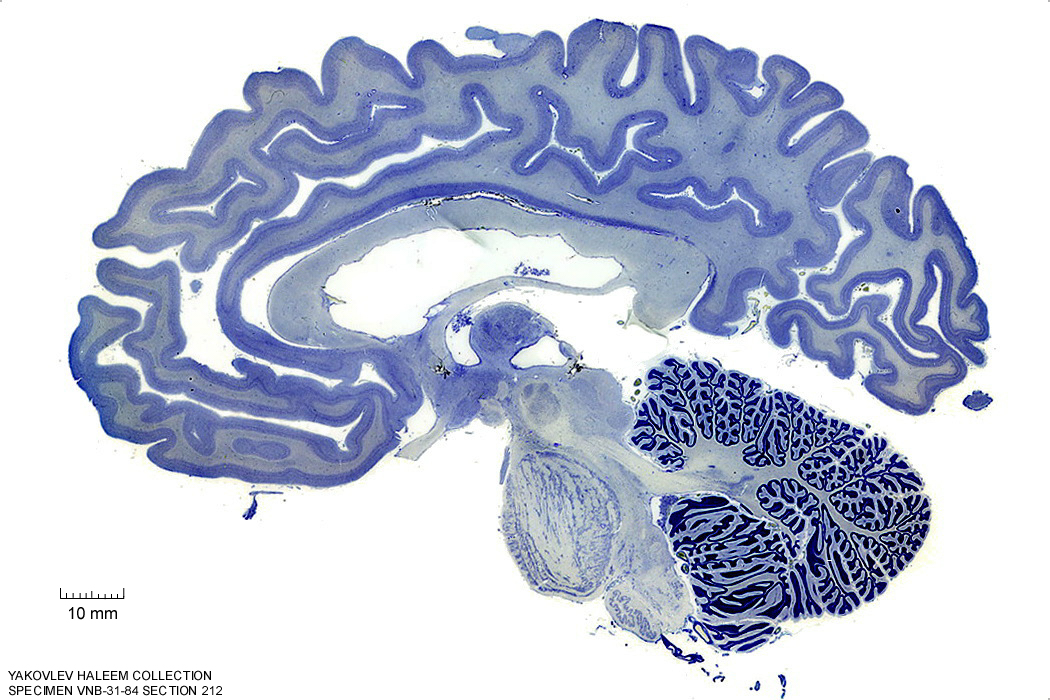
\includegraphics[width=0.7\linewidth]{./figures/cns/0212_cell} 

}

\caption{Sagittal section from \href{https://msu.edu/~brains/brains/human/index.html}{The Human Brain Atlas} at the \href{https://msu.edu/~brains/copyright.html}{Michigan State University Brain Biodiveristy Bank} which \href{https://msu.edu/~brains/copyright.html}{acknowledges} their support from the National Science Foundation.}\label{fig:212}
\end{figure}

In Figure \ref{fig:182}, label the following structures:

\begin{enumerate}
\def\labelenumi{\arabic{enumi}.}
\tightlist
\item
  The corpus callosum
\end{enumerate}

\begin{itemize}
\tightlist
\item
  the splenium
\item
  the body
\item
  the genu
\end{itemize}

\begin{enumerate}
\def\labelenumi{\arabic{enumi}.}
\tightlist
\item
  The thalamus
\item
  The anterior commissure
\item
  The optic chiasm
\item
  The lamina terminalis
\item
  The mammillothalamic tract
\item
  The mammillariy nuclei
\item
  The hypothalamus
\item
  The red nucleus
\item
  The cerebral peduncle
\item
  The superior colliculus
\item
  The inferior colliculus
\item
  The pontine nuclei
\item
  The inferior olive
\item
  The cerebellar tonsil
\item
  The decussation of the superior cerebellar peduncle
\item
  The cerebellum
\item
  The fornix
\item
  The habenular commissure
\item
  The septum lucidum
\item
  The periaqueductal grey matter
\item
  The precuneus
\item
  The cuneus
\item
  The fornix
\item
  The lateral ventricle
\item
  The parieto-occipital sulcus
\item
  The lingual gyrus
\item
  The calcarine sulcus
\item
  The cingulate sulcus
\item
  The cingulate gyrus
\item
  The cerebellum
\end{enumerate}



\begin{figure}

{\centering 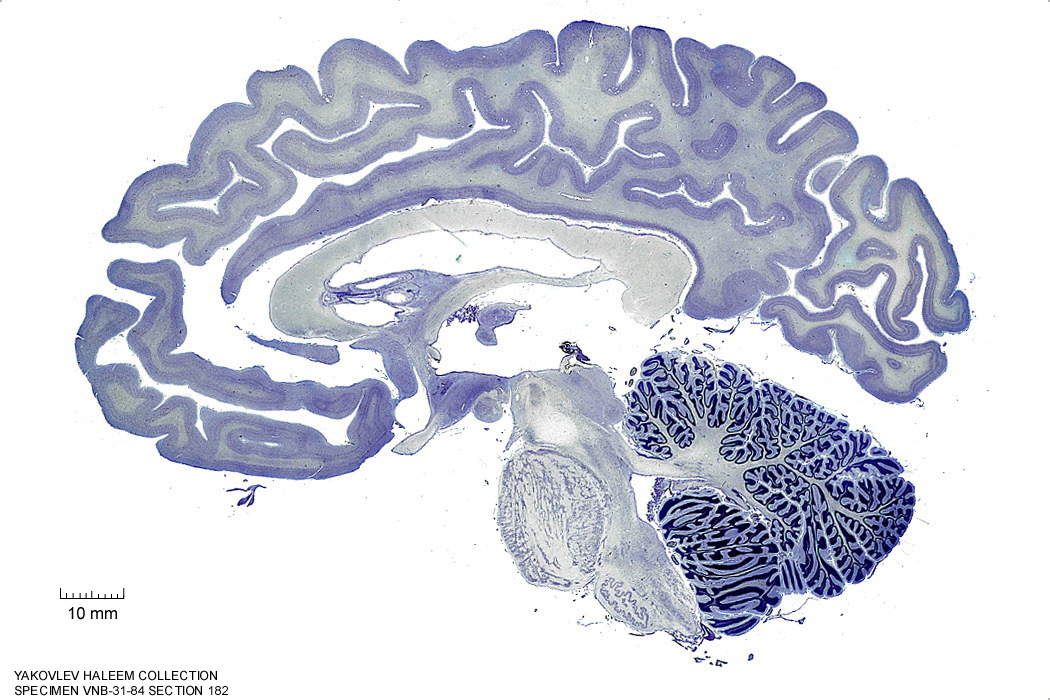
\includegraphics[width=0.7\linewidth]{./figures/cns/0182_cell} 

}

\caption{Sagittal section from \href{https://msu.edu/~brains/brains/human/index.html}{The Human Brain Atlas} at the \href{https://msu.edu/~brains/copyright.html}{Michigan State University Brain Biodiveristy Bank} which \href{https://msu.edu/~brains/copyright.html}{acknowledges} their support from the National Science Foundation.}\label{fig:182}
\end{figure}

In Figure \ref{fig:152}, label the following structures:

\begin{enumerate}
\def\labelenumi{\arabic{enumi}.}
\tightlist
\item
  The corpus callosum
\end{enumerate}

\begin{itemize}
\tightlist
\item
  the splenium
\item
  the body
\item
  the genu
\end{itemize}

\begin{enumerate}
\def\labelenumi{\arabic{enumi}.}
\tightlist
\item
  The thalamus
\item
  The anterior commissure
\item
  The optic chiasm
\item
  The lamina terminalis
\item
  The mammillothalamic tract
\item
  The mammillariy nuclei
\item
  The hypothalamus
\item
  The red nucleus
\item
  The cerebral peduncle
\item
  The superior colliculus
\item
  The inferior colliculus
\item
  The pontine nuclei
\item
  The inferior olive
\item
  The cerebellar tonsil
\item
  The decussation of the superior cerebellar peduncle
\item
  The cerebellum
\item
  The fornix
\item
  The habenular commissure
\item
  The septum lucidum
\item
  The periaqueductal grey matter
\item
  The precuneus
\item
  The cuneus
\item
  The fornix
\item
  The lateral ventricle
\item
  The parieto-occipital sulcus
\item
  The gracile nucleus
\item
  The cuneate fasciculus
\item
  The 4\textsuperscript{th} ventricle
\item
  The lingual gyrus
\item
  The calcarine sulcus
\item
  The cingulate sulcus
\item
  The cingulate gyrus
\item
  The cerebellum
\item
  The cerebral aqueduct
\item
  The posterior commissure
\end{enumerate}



\begin{figure}

{\centering 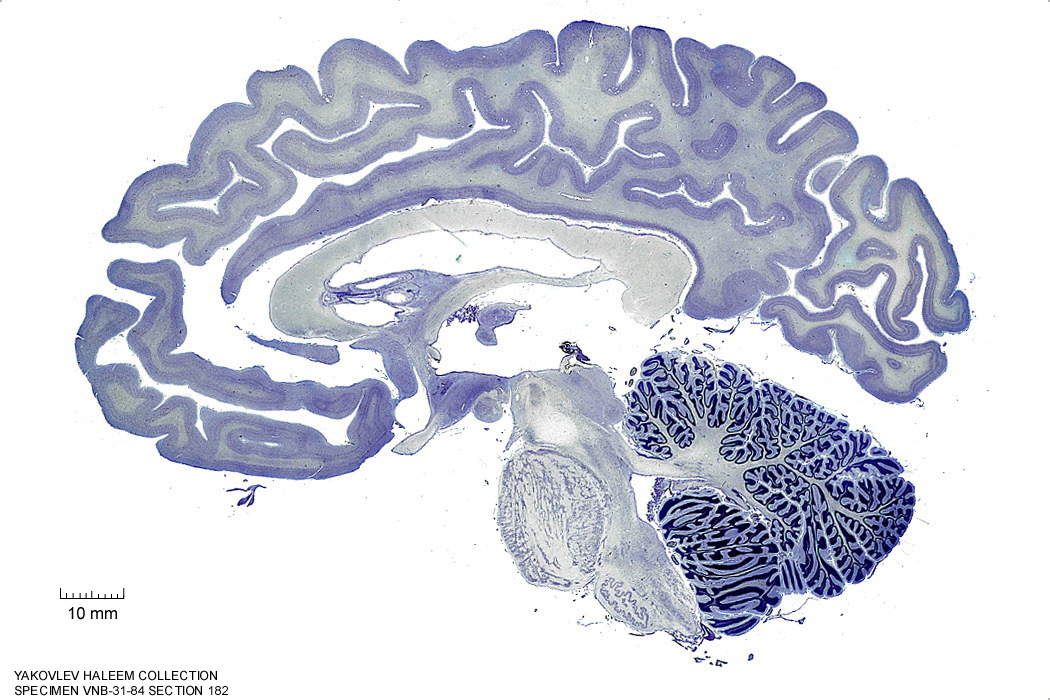
\includegraphics[width=0.7\linewidth]{./figures/cns/0182_cell} 

}

\caption{Sagittal section from \href{https://msu.edu/~brains/brains/human/index.html}{The Human Brain Atlas} at the \href{https://msu.edu/~brains/copyright.html}{Michigan State University Brain Biodiveristy Bank} which \href{https://msu.edu/~brains/copyright.html}{acknowledges} their support from the National Science Foundation.}\label{fig:152}
\end{figure}

\hypertarget{a-series-of-horizontal-sections-of-a-human-brain}{%
\section{A Series Of Horizontal Sections Of A Human Brain}\label{a-series-of-horizontal-sections-of-a-human-brain}}

In Figure \ref{fig:800}, label the following structures:

\begin{enumerate}
\def\labelenumi{\arabic{enumi}.}
\tightlist
\item
  The middle frontal gyrus
\item
  The superior frontal gyrus
\item
  The superior frontal sulcus
\item
  The medial longitudinal fissure
\item
  The precuneus
\item
  The cingulate gyrus
\item
  The precentral sulcus
\item
  The precentral gyrus
\item
  The central sulcus
\item
  The postcentral gyrus
\item
  The postcentral sulcus
\item
  The supramarginal gyrus
\item
  The intraparietal sulcus
\item
  The superior parietal lobule
\item
  The parieto-occipital sulcus
\item
  The intraparietal sulcus
\end{enumerate}



\begin{figure}

{\centering 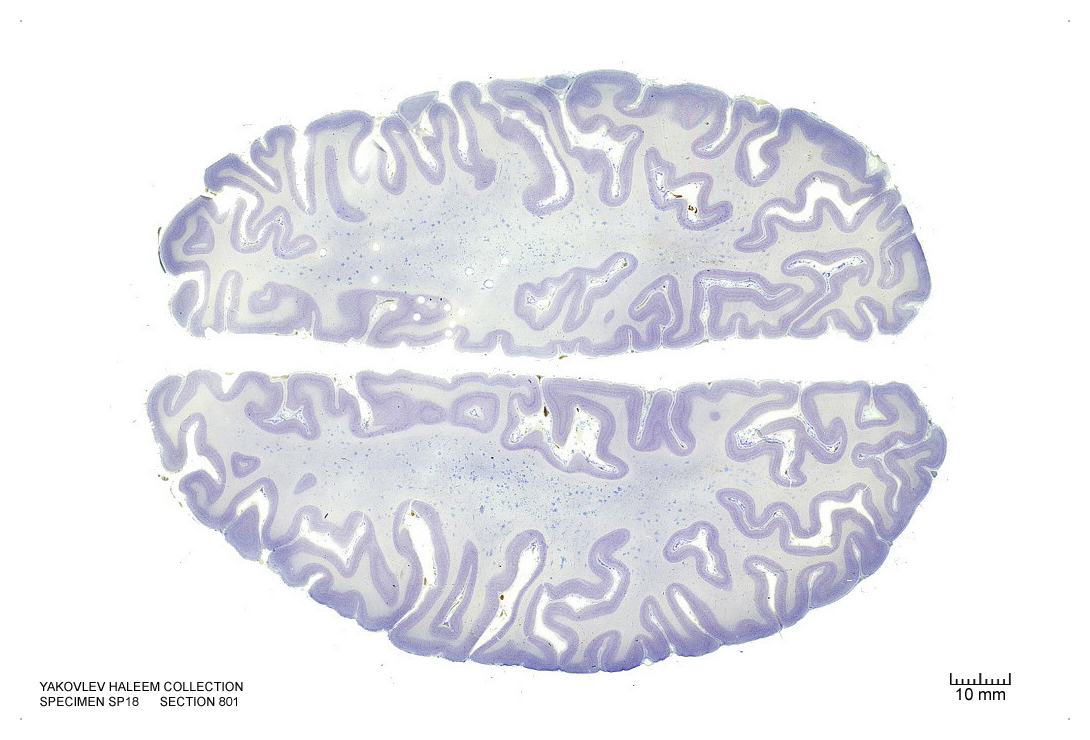
\includegraphics[width=0.7\linewidth]{./figures/cns/horizontal/0800_cell} 

}

\caption{Horizontal section from \href{https://msu.edu/~brains/brains/human/index.html}{The Human Brain Atlas} at the \href{https://msu.edu/~brains/copyright.html}{Michigan State University Brain Biodiveristy Bank} which \href{https://msu.edu/~brains/copyright.html}{acknowledges} their support from the National Science Foundation.}\label{fig:800}
\end{figure}

In Figure \ref{fig:940}, label the following structures:

\begin{enumerate}
\def\labelenumi{\arabic{enumi}.}
\tightlist
\item
  The middle frontal gyrus
\item
  The inferior frontal gyrus
\item
  The inferior frontal sulcus
\item
  The medial longitudinal fissure
\item
  The precuneus
\item
  The cingulate gyrus
\item
  The cingulate sulcus
\item
  The superior frontal gyrus
\item
  The superior frontal sulcus
\item
  The angular gyrus
\item
  The precentral sulcus
\item
  The precentral gyrus
\item
  The central sulcus
\item
  The postcentral gyrus
\item
  The postcentral sulcus
\item
  The supramarginal gyrus
\item
  The intraparietal sulcus
\item
  The superior parietal lobule
\item
  The parieto-occipital sulcus
\item
  The intraparietal sulcus
\item
  The lateral sulcus
\end{enumerate}



\begin{figure}

{\centering 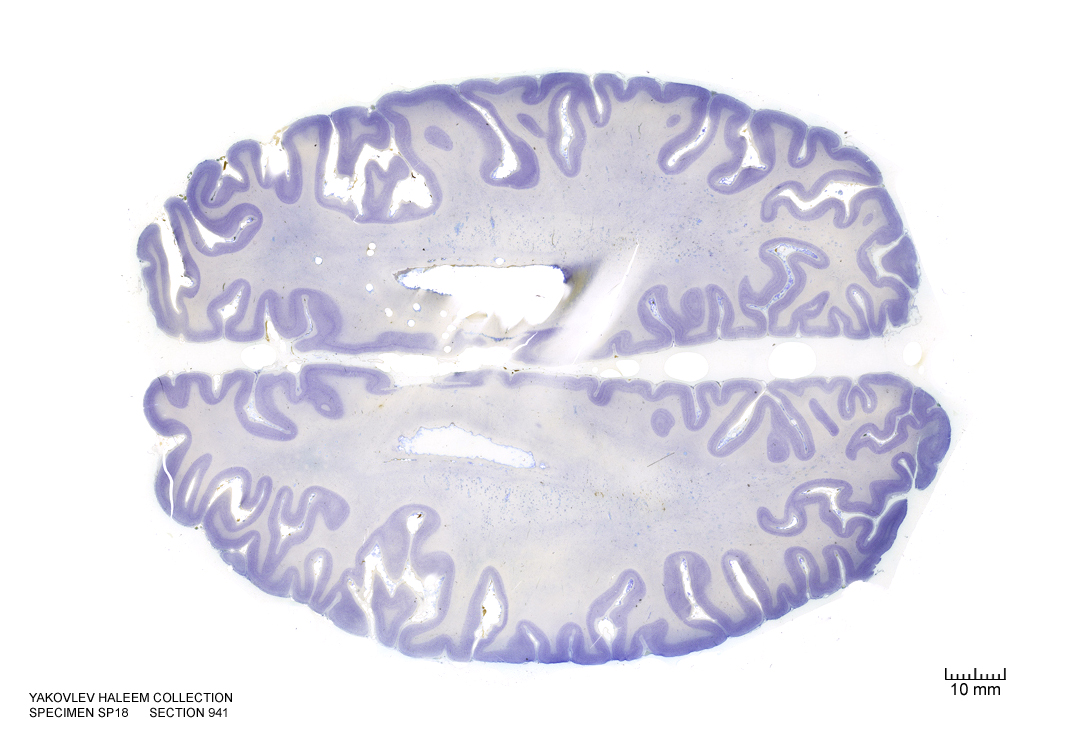
\includegraphics[width=0.7\linewidth]{./figures/cns/horizontal/0940_cell} 

}

\caption{Horizontal section from \href{https://msu.edu/~brains/brains/human/index.html}{The Human Brain Atlas} at the \href{https://msu.edu/~brains/copyright.html}{Michigan State University Brain Biodiveristy Bank} which \href{https://msu.edu/~brains/copyright.html}{acknowledges} their support from the National Science Foundation.}\label{fig:940}
\end{figure}

In Figure \ref{fig:1000}, label the following structures:

\begin{enumerate}
\def\labelenumi{\arabic{enumi}.}
\tightlist
\item
  The middle frontal gyrus
\item
  The inferior frontal gyrus
\item
  The inferior frontal sulcus
\item
  The medial longitudinal fissure
\item
  The precuneus
\item
  The cuneus
\item
  The cingulate gyrus
\item
  The cingulate sulcus
\item
  The superior frontal gyrus
\item
  The superior frontal sulcus
\item
  The angular gyrus
\item
  The precentral sulcus
\item
  The precentral gyrus
\item
  The central sulcus
\item
  The postcentral gyrus
\item
  The postcentral sulcus
\item
  The supramarginal gyrus
\item
  The intraparietal sulcus
\item
  The superior parietal lobule
\item
  The parieto-occipital sulcus
\item
  The intraparietal sulcus
\item
  the lateral sulcus
\end{enumerate}



\begin{figure}

{\centering 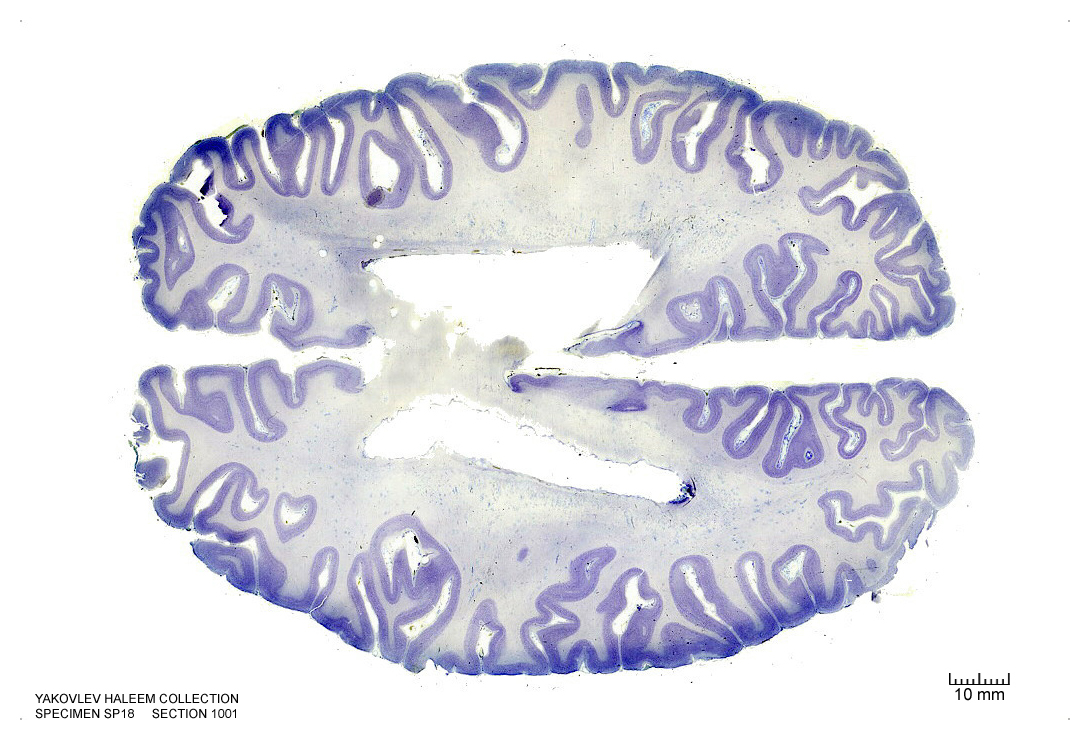
\includegraphics[width=0.7\linewidth]{./figures/cns/horizontal/1000_cell} 

}

\caption{Horizontal section from \href{https://msu.edu/~brains/brains/human/index.html}{The Human Brain Atlas} at the \href{https://msu.edu/~brains/copyright.html}{Michigan State University Brain Biodiveristy Bank} which \href{https://msu.edu/~brains/copyright.html}{acknowledges} their support from the National Science Foundation.}\label{fig:1000}
\end{figure}

In Figure \ref{fig:1100}, label the following structures:

\begin{enumerate}
\def\labelenumi{\arabic{enumi}.}
\tightlist
\item
  The middle frontal gyrus
\item
  The inferior frontal gyrus
\item
  The inferior frontal sulcus
\item
  The medial longitudinal fissure
\item
  The precuneus
\item
  The cuneus
\item
  The cingulate gyrus
\item
  The cingulate sulcus
\item
  The callosal sulcus
\item
  The lateral ventricle
\item
  The septum pellucidum
\item
  The insula
\item
  The corpus callosum
\item
  The superior frontal gyrus
\item
  The superior frontal sulcus
\item
  The angular gyrus
\item
  The precentral sulcus
\item
  The precentral gyrus
\item
  The central sulcus
\item
  The postcentral gyrus
\item
  The postcentral sulcus
\item
  The supramarginal gyrus
\item
  The intraparietal sulcus
\item
  The superior parietal lobule
\item
  The parieto-occipital sulcus
\item
  The intraparietal sulcus
\item
  the lateral sulcus
\end{enumerate}



\begin{figure}

{\centering 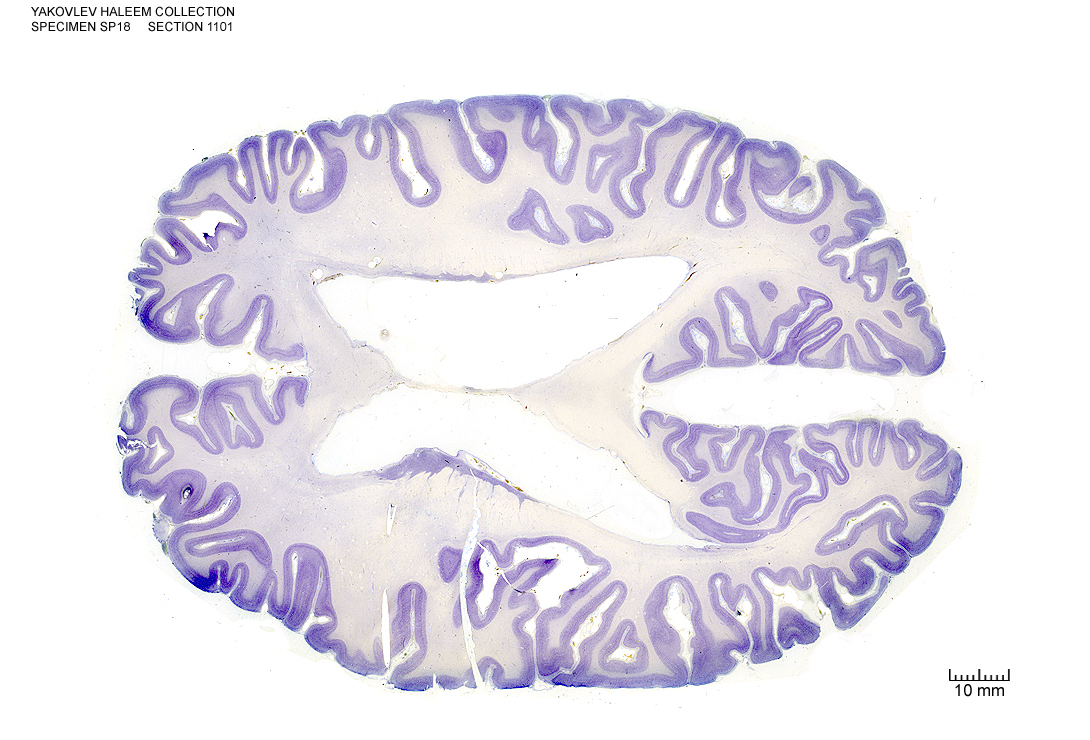
\includegraphics[width=0.7\linewidth]{./figures/cns/horizontal/1100_cell} 

}

\caption{(ref:h11100)}\label{fig:1100}
\end{figure}

In Figure \ref{fig:1200}, label the following structures:

\begin{enumerate}
\def\labelenumi{\arabic{enumi}.}
\tightlist
\item
  The sulcus of the corpus callosum
\item
  The splenium of the corpus callosum
\item
  The lateral ventricle
\item
  The septum pellucidum
\item
  The insular cortex
\item
  The head of the caudate nucleus
\item
  The body of the caudate nucleus
\item
  The external capsule
\item
  The putamen
\item
  The tail of the caudate nucleus
\item
  The occipital horn of the lateral ventricle
\item
  The fornix
\item
  The medial longitudinal fissure
\end{enumerate}



\begin{figure}

{\centering 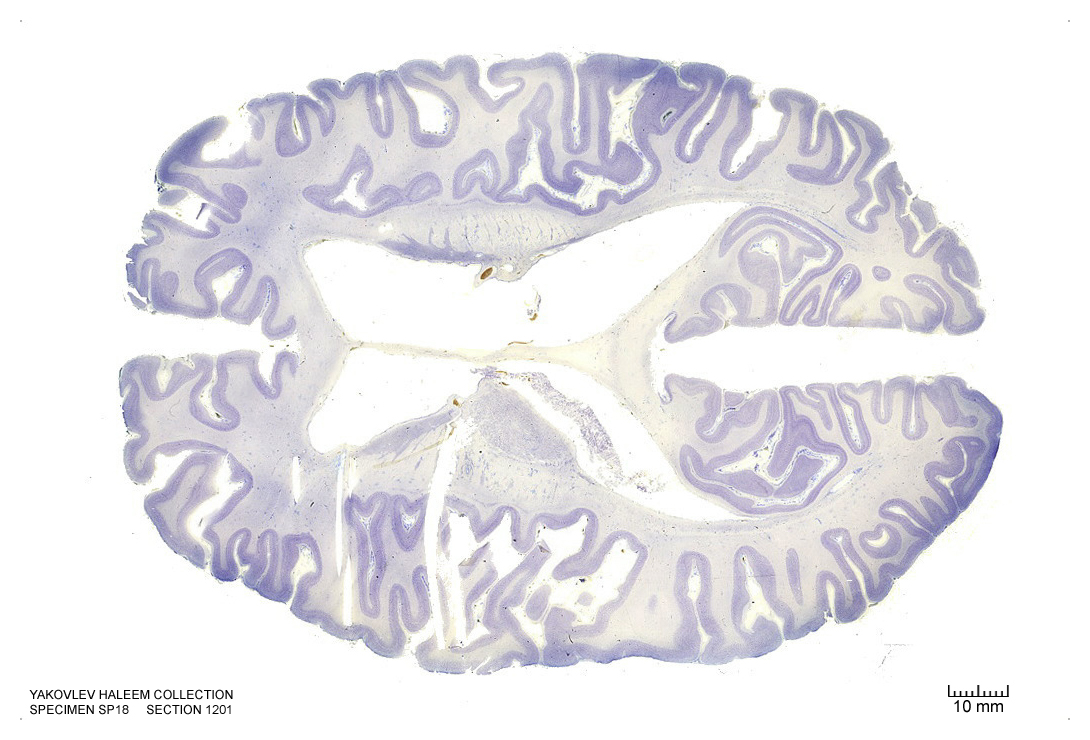
\includegraphics[width=0.7\linewidth]{./figures/cns/horizontal/1200_cell} 

}

\caption{Horizontal section from \href{https://msu.edu/~brains/brains/human/index.html}{The Human Brain Atlas} at the \href{https://msu.edu/~brains/copyright.html}{Michigan State University Brain Biodiveristy Bank} which \href{https://msu.edu/~brains/copyright.html}{acknowledges} their support from the National Science Foundation.}\label{fig:1200}
\end{figure}

In Figure \ref{fig:1300}, label the following structures:

\begin{enumerate}
\def\labelenumi{\arabic{enumi}.}
\tightlist
\item
  The thalamic nuclei
\end{enumerate}

\begin{itemize}
\tightlist
\item
  reticular
\item
  ventroposterior
\item
  ventroanterior
\item
  ventrolateral
\item
  mediodorsal
\item
  anteroprincipal
\end{itemize}

\begin{enumerate}
\def\labelenumi{\arabic{enumi}.}
\tightlist
\item
  The lateral ventricle
\item
  The choroid plexus
\item
  The splenium of the corpus callosum
\item
  The lateral ventricle
\item
  The septum pellucidum
\item
  The insular cortex
\item
  The head of the caudate nucleus
\item
  The body of the caudate nucleus
\item
  The tail of the caudate nucleus
\item
  The external capsule
\item
  The putamen
\item
  The occipital horn of the lateral ventricle
\item
  The fornix
\item
  The medial longitudinal fissure
\item
  The vermis of the cerebellum
\item
  The dentate gyrus
\item
  The internal capsule
\item
  The subiculum
\item
  The primary visual cortex
\item
  The calcarine sulcus
\item
  The fornix
\item
  The cingulate sulcus
\item
  The cingulate gyrus
\item
  The genu of the corpus callosum
\end{enumerate}



\begin{figure}

{\centering 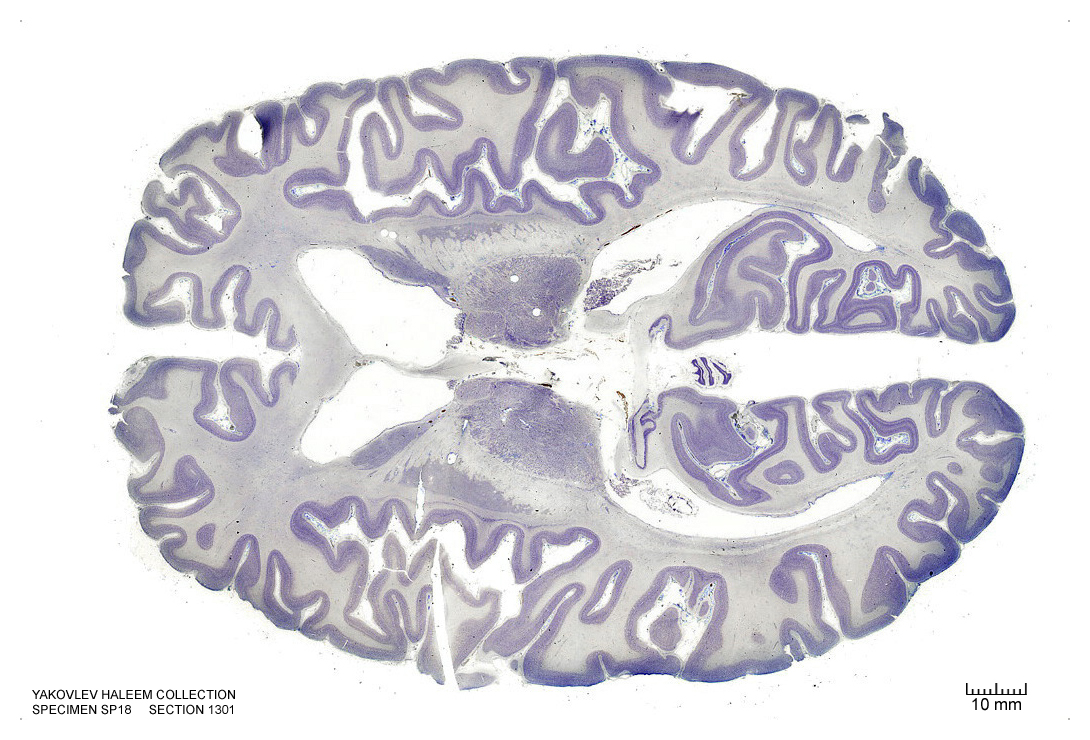
\includegraphics[width=0.7\linewidth]{./figures/cns/horizontal/1300_cell} 

}

\caption{Horizontal section from \href{https://msu.edu/~brains/brains/human/index.html}{The Human Brain Atlas} at the \href{https://msu.edu/~brains/copyright.html}{Michigan State University Brain Biodiveristy Bank} which \href{https://msu.edu/~brains/copyright.html}{acknowledges} their support from the National Science Foundation.}\label{fig:1300}
\end{figure}

In Figure \ref{fig:1400}, label the following structures:

\begin{enumerate}
\def\labelenumi{\arabic{enumi}.}
\tightlist
\item
  The thalamic nuclei
\end{enumerate}

\begin{itemize}
\tightlist
\item
  pulvinar
\item
  reticular
\item
  ventroposterior
\item
  ventroanterior
\item
  ventrolateral
\item
  mediodorsal
\end{itemize}

\begin{enumerate}
\def\labelenumi{\arabic{enumi}.}
\tightlist
\item
  The habenula
\item
  The lateral ventricle
\item
  The septum pellucidum
\item
  The insular cortex
\item
  The head of the caudate nucleus
\item
  The tail of the caudate nucleus
\item
  The external capsule
\item
  The fornix
\item
  The septal nuclei
\item
  The medial longitudinal fissure
\item
  The vermis of the cerebellum
\item
  The dentate gyrus
\item
  The subiculum
\item
  The primary visual cortex
\item
  The calcarine sulcus
\item
  The choroid plexus
\item
  The superior temporal gyrus
\item
  The putamen
\end{enumerate}



\begin{figure}

{\centering 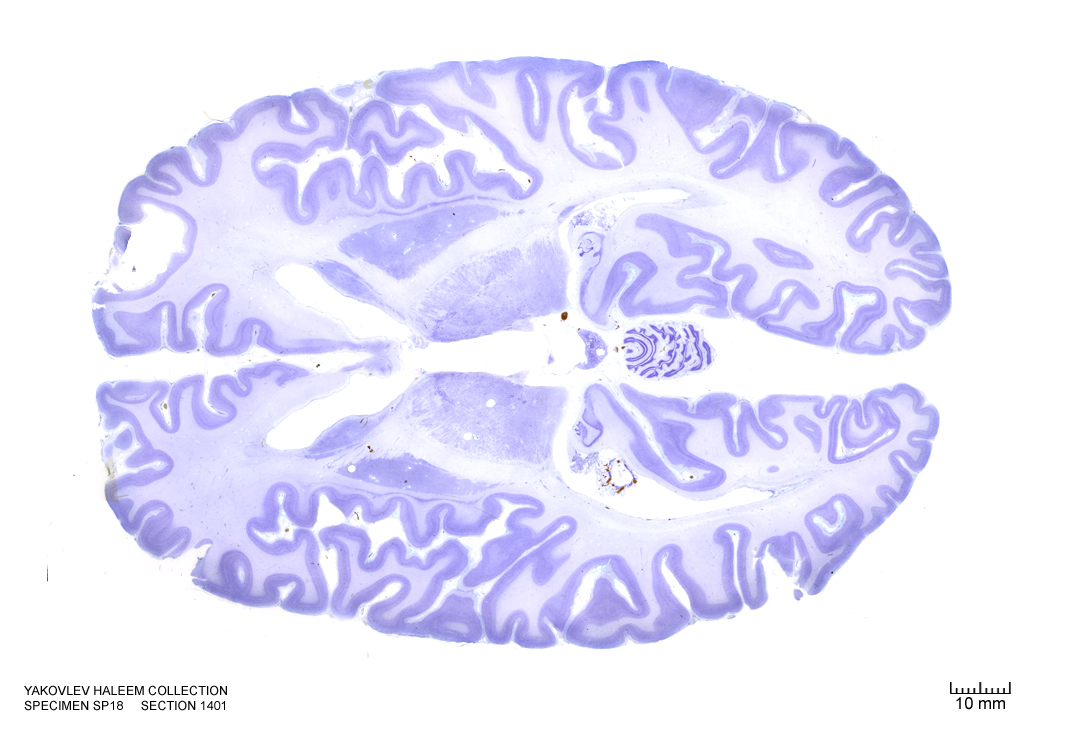
\includegraphics[width=0.7\linewidth]{./figures/cns/horizontal/1400_cell} 

}

\caption{Horizontal section from \href{https://msu.edu/~brains/brains/human/index.html}{The Human Brain Atlas} at the \href{https://msu.edu/~brains/copyright.html}{Michigan State University Brain Biodiveristy Bank} which \href{https://msu.edu/~brains/copyright.html}{acknowledges} their support from the National Science Foundation.}\label{fig:1400}
\end{figure}

In Figure \ref{fig:1500}, label the following structures:

\begin{enumerate}
\def\labelenumi{\arabic{enumi}.}
\tightlist
\item
  The thalamic nuclei
\end{enumerate}

\begin{itemize}
\tightlist
\item
  pulvinar
\item
  reticular
\end{itemize}

\begin{enumerate}
\def\labelenumi{\arabic{enumi}.}
\tightlist
\item
  The 3\textsuperscript{d} ventricle
\item
  The fimbria of the hippocampus
\item
  The claustrum
\item
  The medial geniculate nucleus
\item
  The lateral geniculate nucleus
\item
  The superior colliculus
\item
  The cerebellum
\item
  The head of the caudate nucleus
\item
  The tail of the caudate nucleus
\item
  The external capsule
\item
  The fornix
\item
  The septal nuclei
\item
  The medial longitudinal fissure
\item
  The cerebellum
\item
  The dentate gyrus
\item
  The hippocampus
\item
  The subiculum
\item
  The optic tract
\item
  The insular cortex
\item
  The primary visual cortex
\item
  The calcarine sulcus
\item
  The choroid plexus
\item
  The superior temporal gyrus
\item
  The putamen
\end{enumerate}



\begin{figure}

{\centering \includegraphics[width=0.7\linewidth]{./figures/cns/horizontal/1500_cell} 

}

\caption{Horizontal section from \href{https://msu.edu/~brains/brains/human/index.html}{The Human Brain Atlas} at the \href{https://msu.edu/~brains/copyright.html}{Michigan State University Brain Biodiveristy Bank} which \href{https://msu.edu/~brains/copyright.html}{acknowledges} their support from the National Science Foundation.}\label{fig:1500}
\end{figure}

In Figure \ref{fig:1600}, label the following structures:

\begin{enumerate}
\def\labelenumi{\arabic{enumi}.}
\tightlist
\item
  The cerebral aqueduct
\item
  The mammillothalamic tract
\item
  The red nucleus
\item
  The choroid plexus
\item
  The cerebral peduncle
\item
  The fimbria of the hippocampus
\item
  The medial geniculate nucleus
\item
  The lateral geniculate nucleus
\item
  The inferior colliculus
\item
  The cerebellum
\item
  The vermis of the cerebellum
\item
  The external capsule
\item
  The claustrum
\item
  The ventral striatum
\item
  The medial longitudinal fissure
\item
  The vermis of the cerebellum
\item
  The dentate gyrus
\item
  The hippocampus
\item
  The subiculum
\item
  The optic tract
\item
  The insular cortex
\item
  The primary visual cortex
\item
  The calcarine sulcus
\item
  The substantia nigra
\item
  The fornix
\item
  The optic tract
\item
  The external capsule
\end{enumerate}



\begin{figure}

{\centering \includegraphics[width=0.7\linewidth]{./figures/cns/horizontal/1600_cell} 

}

\caption{Horizontal section from \href{https://msu.edu/~brains/brains/human/index.html}{The Human Brain Atlas} at the \href{https://msu.edu/~brains/copyright.html}{Michigan State University Brain Biodiveristy Bank} which \href{https://msu.edu/~brains/copyright.html}{acknowledges} their support from the National Science Foundation.}\label{fig:1600}
\end{figure}

In Figure \ref{fig:1640}, label the following structures:

\begin{enumerate}
\def\labelenumi{\arabic{enumi}.}
\tightlist
\item
  The cerebral aqueduct
\item
  The red nucleus
\item
  The choroid plexus
\item
  The cerebral peduncle
\item
  The dorsal raphe nucleus
\item
  The periaqueductal grey area
\item
  The 3\textsuperscript{d} ventricle
\item
  The fimbria of the hippocampus
\item
  The medial geniculate nucleus
\item
  The lateral geniculate nucleus
\item
  The inferior colliculus
\item
  The cerebellum
\item
  The vermis of the cerebellum
\item
  The external capsule
\item
  The claustrum
\item
  The ventral striatum
\item
  The medial longitudinal fissure
\item
  The vermis of the cerebellum
\item
  The dentate gyrus
\item
  The hippocampus
\item
  The subiculum
\item
  The optic tract
\item
  The insular cortex
\item
  The primary visual cortex
\item
  The substantia nigra
\item
  The medial lemniscus
\item
  The amygdala
\item
  The orbital gyri
\item
  The ventromedial hypothalamic nucleus
\item
  The ventral striatum
\item
  The fornix
\item
  The optic tract
\item
  The external capsule
\end{enumerate}



\begin{figure}

{\centering \includegraphics[width=0.7\linewidth]{./figures/cns/horizontal/1640_cell} 

}

\caption{Horizontal section from \href{https://msu.edu/~brains/brains/human/index.html}{The Human Brain Atlas} at the \href{https://msu.edu/~brains/copyright.html}{Michigan State University Brain Biodiveristy Bank} which \href{https://msu.edu/~brains/copyright.html}{acknowledges} their support from the National Science Foundation.}\label{fig:1640}
\end{figure}

In Figure \ref{fig:1700}, label the following structures:

\begin{enumerate}
\def\labelenumi{\arabic{enumi}.}
\tightlist
\item
  The cerebral aqueduct
\item
  The red nucleus
\item
  The choroid plexus
\item
  The cerebral peduncle
\item
  The dorsal raphe nucleus
\item
  The periaqueductal grey area
\item
  The 3\textsuperscript{d} ventricle
\item
  The fimbria of the hippocampus
\item
  The medial geniculate nucleus
\item
  The lateral geniculate nucleus
\item
  The inferior colliculus
\item
  The cerebellum
\item
  The vermis of the cerebellum
\item
  The external capsule
\item
  The claustrum
\item
  The ventral striatum
\item
  The medial longitudinal fissure
\item
  The vermis of the cerebellum
\item
  The dentate gyrus
\item
  The hippocampus
\item
  The subiculum
\item
  The optic tract
\item
  The insular cortex
\item
  The primary visual cortex
\item
  The substantia nigra
\item
  The medial lemniscus
\item
  The amygdala
\item
  The orbital gyri
\item
  The ventromedial hypothalamic nucleus
\item
  The ventral striatum
\item
  The fornix
\item
  The optic tract
\item
  The external capsule
\end{enumerate}



\begin{figure}

{\centering \includegraphics[width=0.7\linewidth]{./figures/cns/horizontal/1700_cell} 

}

\caption{Horizontal section from \href{https://msu.edu/~brains/brains/human/index.html}{The Human Brain Atlas} at the \href{https://msu.edu/~brains/copyright.html}{Michigan State University Brain Biodiveristy Bank} which \href{https://msu.edu/~brains/copyright.html}{acknowledges} their support from the National Science Foundation.}\label{fig:1700}
\end{figure}

In Figure \ref{fig:1740}, label the following structures:



\begin{figure}

{\centering \includegraphics[width=0.7\linewidth]{./figures/cns/horizontal/1740_cell} 

}

\caption{Horizontal section from \href{https://msu.edu/~brains/brains/human/index.html}{The Human Brain Atlas} at the \href{https://msu.edu/~brains/copyright.html}{Michigan State University Brain Biodiveristy Bank} which \href{https://msu.edu/~brains/copyright.html}{acknowledges} their support from the National Science Foundation.}\label{fig:1740}
\end{figure}

In Figure \ref{fig:1800}, label the following structures:



\begin{figure}

{\centering \includegraphics[width=0.7\linewidth]{./figures/cns/horizontal/1800_cell} 

}

\caption{Horizontal section from \href{https://msu.edu/~brains/brains/human/index.html}{The Human Brain Atlas} at the \href{https://msu.edu/~brains/copyright.html}{Michigan State University Brain Biodiveristy Bank} which \href{https://msu.edu/~brains/copyright.html}{acknowledges} their support from the National Science Foundation.}\label{fig:1800}
\end{figure}

In Figure \ref{fig:ho1840}, label the following structures:



\begin{figure}

{\centering \includegraphics[width=0.7\linewidth]{./figures/cns/horizontal/1840_cell} 

}

\caption{Horizontal section from \href{https://msu.edu/~brains/brains/human/index.html}{The Human Brain Atlas} at the \href{https://msu.edu/~brains/copyright.html}{Michigan State University Brain Biodiveristy Bank} which \href{https://msu.edu/~brains/copyright.html}{acknowledges} their support from the National Science Foundation.}\label{fig:ho1840}
\end{figure}

In Figure \ref{fig:1900}, label the following structures:



\begin{figure}

{\centering \includegraphics[width=0.7\linewidth]{./figures/cns/horizontal/1900_cell} 

}

\caption{Horizontal section from \href{https://msu.edu/~brains/brains/human/index.html}{The Human Brain Atlas} at the \href{https://msu.edu/~brains/copyright.html}{Michigan State University Brain Biodiveristy Bank} which \href{https://msu.edu/~brains/copyright.html}{acknowledges} their support from the National Science Foundation.}\label{fig:1900}
\end{figure}

In Figure \ref{fig:ho2000}, label the following structures:



\begin{figure}

{\centering \includegraphics[width=0.7\linewidth]{./figures/cns/horizontal/2000_cell} 

}

\caption{Horizontal section from \href{https://msu.edu/~brains/brains/human/index.html}{The Human Brain Atlas} at the \href{https://msu.edu/~brains/copyright.html}{Michigan State University Brain Biodiveristy Bank} which \href{https://msu.edu/~brains/copyright.html}{acknowledges} their support from the National Science Foundation.}\label{fig:ho2000}
\end{figure}

In Figure \ref{fig:2100}, label the following structures:



\begin{figure}

{\centering \includegraphics[width=0.7\linewidth]{./figures/cns/horizontal/2100_cell} 

}

\caption{Horizontal section from \href{https://msu.edu/~brains/brains/human/index.html}{The Human Brain Atlas} at the \href{https://msu.edu/~brains/copyright.html}{Michigan State University Brain Biodiveristy Bank} which \href{https://msu.edu/~brains/copyright.html}{acknowledges} their support from the National Science Foundation.}\label{fig:2100}
\end{figure}

In Figure \ref{fig:2200}, label the following structures:



\begin{figure}

{\centering \includegraphics[width=0.7\linewidth]{./figures/cns/horizontal/2200_cell} 

}

\caption{Horizontal section from \href{https://msu.edu/~brains/brains/human/index.html}{The Human Brain Atlas} at the \href{https://msu.edu/~brains/copyright.html}{Michigan State University Brain Biodiveristy Bank} which \href{https://msu.edu/~brains/copyright.html}{acknowledges} their support from the National Science Foundation.}\label{fig:2200}
\end{figure}

In Figure \ref{fig:ho2240}, label the following structures:



\begin{figure}

{\centering \includegraphics[width=0.7\linewidth]{./figures/cns/horizontal/2240_cell} 

}

\caption{Horizontal section from \href{https://msu.edu/~brains/brains/human/index.html}{The Human Brain Atlas} at the \href{https://msu.edu/~brains/copyright.html}{Michigan State University Brain Biodiveristy Bank} which \href{https://msu.edu/~brains/copyright.html}{acknowledges} their support from the National Science Foundation.}\label{fig:ho2240}
\end{figure}

In Figure \ref{fig:2260}, label the following structures:



\begin{figure}

{\centering \includegraphics[width=0.7\linewidth]{./figures/cns/horizontal/2260_cell} 

}

\caption{Horizontal section from \href{https://msu.edu/~brains/brains/human/index.html}{The Human Brain Atlas} at the \href{https://msu.edu/~brains/copyright.html}{Michigan State University Brain Biodiveristy Bank} which \href{https://msu.edu/~brains/copyright.html}{acknowledges} their support from the National Science Foundation.}\label{fig:2260}
\end{figure}

In Figure \ref{fig:2280}, label the following structures:



\begin{figure}

{\centering \includegraphics[width=0.7\linewidth]{./figures/cns/horizontal/2280_cell} 

}

\caption{Horizontal section from \href{https://msu.edu/~brains/brains/human/index.html}{The Human Brain Atlas} at the \href{https://msu.edu/~brains/copyright.html}{Michigan State University Brain Biodiveristy Bank} which \href{https://msu.edu/~brains/copyright.html}{acknowledges} their support from the National Science Foundation.}\label{fig:2280}
\end{figure}

In Figure \ref{fig:2300}, label the following structures:



\begin{figure}

{\centering \includegraphics[width=0.7\linewidth]{./figures/cns/horizontal/2300_cell} 

}

\caption{Horizontal section from \href{https://msu.edu/~brains/brains/human/index.html}{The Human Brain Atlas} at the \href{https://msu.edu/~brains/copyright.html}{Michigan State University Brain Biodiveristy Bank} which \href{https://msu.edu/~brains/copyright.html}{acknowledges} their support from the National Science Foundation.}\label{fig:2300}
\end{figure}

In Figure \ref{fig:2340}, label the following structures:



\begin{figure}

{\centering \includegraphics[width=0.7\linewidth]{./figures/cns/horizontal/2340_cell} 

}

\caption{Horizontal section from \href{https://msu.edu/~brains/brains/human/index.html}{The Human Brain Atlas} at the \href{https://msu.edu/~brains/copyright.html}{Michigan State University Brain Biodiveristy Bank} which \href{https://msu.edu/~brains/copyright.html}{acknowledges} their support from the National Science Foundation.}\label{fig:2340}
\end{figure}

In Figure \ref{fig:2400}, label the following structures:



\begin{figure}

{\centering \includegraphics[width=0.7\linewidth]{./figures/cns/horizontal/2400_cell} 

}

\caption{Horizontal section from \href{https://msu.edu/~brains/brains/human/index.html}{The Human Brain Atlas} at the \href{https://msu.edu/~brains/copyright.html}{Michigan State University Brain Biodiveristy Bank} which \href{https://msu.edu/~brains/copyright.html}{acknowledges} their support from the National Science Foundation.}\label{fig:2400}
\end{figure}

In Figure \ref{fig:2440}, label the following structures:



\begin{figure}

{\centering \includegraphics[width=0.7\linewidth]{./figures/cns/horizontal/2440_cell} 

}

\caption{Horizontal section from \href{https://msu.edu/~brains/brains/human/index.html}{The Human Brain Atlas} at the \href{https://msu.edu/~brains/copyright.html}{Michigan State University Brain Biodiveristy Bank} which \href{https://msu.edu/~brains/copyright.html}{acknowledges} their support from the National Science Foundation.}\label{fig:2440}
\end{figure}

In Figure \ref{fig:2480}, label the following structures:



\begin{figure}

{\centering \includegraphics[width=0.7\linewidth]{./figures/cns/horizontal/2480_cell} 

}

\caption{Horizontal section from \href{https://msu.edu/~brains/brains/human/index.html}{The Human Brain Atlas} at the \href{https://msu.edu/~brains/copyright.html}{Michigan State University Brain Biodiveristy Bank} which \href{https://msu.edu/~brains/copyright.html}{acknowledges} their support from the National Science Foundation.}\label{fig:2480}
\end{figure}

\hypertarget{the-diencephalon}{%
\chapter{The Diencephalon}\label{the-diencephalon}}

In this laboratory session, we will study the anatomy of the human diencephalon. The diencephalon is a division of the forebrain (embryonic prosencephalon), and is situated between the telencephalon and the midbrain (embryonic mesencephalon). It consists of structures that are on either side of the third ventricle, including the thalamus, the hypothalamus, the epithalamus and the subthalamus.

Below, you will be presented with a number of figures and asked to label or color certain structures in each figure.

\hypertarget{a-series-of-coronal-sections-of-a-human-brain-1}{%
\section{A Series Of Coronal Sections Of A Human Brain}\label{a-series-of-coronal-sections-of-a-human-brain-1}}

In Figure \ref{fig:1520}, label the following structures:

\begin{enumerate}
\def\labelenumi{\arabic{enumi}.}
\tightlist
\item
  The cingulate sulcus
\item
  The cingulate gyrus
\item
  The corpus callosum
\item
  The lateral ventricle
\item
  The caudate nucleus
\item
  The insula
\item
  The lateral sulcus
\item
  The superior temporal gyrus
\item
  The superior temporal sulcus
\item
  The middle temporal gyrus
\item
  The middle temporal sulcus
\item
  The inferior temporal gyrus
\item
  The inferior temporal sulcus
\item
  The putamen
\item
  The nucleus accumbens
\item
  The optic nerves (left and right)
\item
  The septum pelucidum
\item
  The septal nuclei
\item
  The internal capsule
\item
  The external capsule
\item
  The entorhinal cortex
\item
  The parahippocampal gyrus
\end{enumerate}

\begin{figure}

{\centering \includegraphics[width=0.7\linewidth]{./figures/cns/1520_cell} 

}

\caption{Coronal section from \href{https://msu.edu/~brains/brains/human/index.html}{The Human Brain Atlas} at the \href{https://msu.edu/~brains/copyright.html}{Michigan State University Brain Biodiveristy Bank} which \href{https://msu.edu/~brains/copyright.html}{acknowledges} their support from the National Science Foundation.}\label{fig:1520}
\end{figure}

In Figure \ref{fig:1680}, label the following structures:

\begin{enumerate}
\def\labelenumi{\arabic{enumi}.}
\tightlist
\item
  The cingulate sulcus
\item
  The cingulate gyrus
\item
  The corpus callosum
\item
  The fornix
\item
  The lateral ventricle
\item
  The choroid plexus
\item
  The anterior commissure
\item
  The insula
\item
  The lateral sulcus
\item
  The superior temporal gyrus
\item
  The superior temporal sulcus
\item
  The middle temporal gyrus
\item
  The middle temporal sulcus
\item
  The inferior temporal gyrus
\item
  The inferior temporal sulcus
\item
  The putamen
\item
  The preoptic area
\item
  The optic chiasm
\item
  The infundibular stalk
\item
  A pigment epithelial cell with extended proces
\item
  The 3\textsuperscript{d} ventricle
\item
  The internal capsule
\item
  The external capsule
\item
  The claustrum
\item
  The globus pallidus
\item
  The anterior commissure
\item
  The amygdala
\item
  The entorhinal cortex
\item
  The parahippocampal gyrus
\end{enumerate}

\begin{figure}

{\centering \includegraphics[width=0.7\linewidth]{./figures/cns/1680_cell} 

}

\caption{Coronal section from \href{https://msu.edu/~brains/brains/human/index.html}{The Human Brain Atlas} at the \href{https://msu.edu/~brains/copyright.html}{Michigan State University Brain Biodiveristy Bank} which \href{https://msu.edu/~brains/copyright.html}{acknowledges} their support from the National Science Foundation.}\label{fig:1680}
\end{figure}

In Figure @ref(fig:\texttt{1840}), label the following structures:

\begin{enumerate}
\def\labelenumi{\arabic{enumi}.}
\tightlist
\item
  The cingulate sulcus
\item
  The cingulate gyrus
\item
  The corpus callosum
\item
  The fornix
\item
  The lateral ventricle
\item
  The choroid plexus
\item
  The caudate nucleus
\item
  The thalamus
\item
  The insula
\item
  The lateral sulcus
\item
  The superior temporal gyrus
\item
  The superior temporal sulcus
\item
  The middle temporal gyrus
\item
  The middle temporal sulcus
\item
  The inferior temporal gyrus
\item
  The inferior temporal sulcus
\item
  The putamen
\item
  The hippocampus
\item
  The 3\textsuperscript{d} ventricle
\item
  The internal capsule
\item
  The external capsule
\item
  The claustrum
\item
  The globus pallidus
\item
  The fornix
\item
  The optic tract
\item
  The hypothalamus
\item
  The lateral ventricle
\item
  The entorhinal cortex
\item
  The parahippocampal gyrus
\item
  The amygdaloid nuclei:

  \begin{itemize}
  \tightlist
  \item
    medial
  \item
    central
  \item
    cortical
  \item
    basomedial
  \item
    basolateral
  \item
    lateral
  \end{itemize}
\end{enumerate}

Coronal section from \href{https://msu.edu/~brains/brains/human/index.html}{The Human Brain Atlas} at the \href{https://msu.edu/~brains/copyright.html}{Michigan State University Brain Biodiveristy Bank} which \href{https://msu.edu/~brains/copyright.html}{acknowledges} their support from the National Science Foundation. Coronal section from \href{https://msu.edu/~brains/brains/human/index.html}{The Human Brain Atlas} at the \href{https://msu.edu/~brains/copyright.html}{Michigan State University Brain Biodiveristy Bank} which \href{https://msu.edu/~brains/copyright.html}{acknowledges} their support from the National Science Foundation.

\begin{figure}

{\centering \includegraphics[width=0.7\linewidth]{./figures/cns/1840_cell} 

}

\caption{Coronal section from \href{https://msu.edu/~brains/brains/human/index.html}{The Human Brain Atlas} at the \href{https://msu.edu/~brains/copyright.html}{Michigan State University Brain Biodiveristy Bank} which \href{https://msu.edu/~brains/copyright.html}{acknowledges} their support from the National Science Foundation.}\label{fig:1840}
\end{figure}

In Figure \ref{fig:2000}, label the following structures:

Coronal section from \href{https://msu.edu/~brains/brains/human/index.html}{The Human Brain Atlas} at the \href{https://msu.edu/~brains/copyright.html}{Michigan State University Brain Biodiveristy Bank} which \href{https://msu.edu/~brains/copyright.html}{acknowledges} their support from the National Science Foundation. Coronal section from \href{https://msu.edu/~brains/brains/human/index.html}{The Human Brain Atlas} at the \href{https://msu.edu/~brains/copyright.html}{Michigan State University Brain Biodiveristy Bank} which \href{https://msu.edu/~brains/copyright.html}{acknowledges} their support from the National Science Foundation.

\begin{enumerate}
\def\labelenumi{\arabic{enumi}.}
\tightlist
\item
  The cingulate sulcus
\item
  The cingulate gyrus
\item
  The corpus callosum
\item
  The fornix
\item
  The lateral ventricle
\item
  The choroid plexus
\item
  The caudate nucleus
\item
  The thalamus
\item
  The insula
\item
  The lateral sulcus
\item
  The superior temporal gyrus
\item
  The superior temporal sulcus
\item
  The middle temporal gyrus
\item
  The middle temporal sulcus
\item
  The inferior temporal gyrus
\item
  The inferior temporal sulcus
\item
  The putamen
\item
  The hippocampus
\item
  The dentate gyrus
\item
  The zona incerta
\item
  The substantia nigra
\item
  The 3\textsuperscript{d} ventricle
\item
  The thalamus
\item
  The internal capsule
\item
  The external capsule
\item
  The claustrum
\item
  The globus pallidus
\item
  The optic tract
\item
  The lateral ventricle
\item
  The subthalamic nucleus
\item
  The entorhinal cortex
\item
  The parahippocampal gyrus
\item
  The cerebral peduncle
\end{enumerate}

\begin{figure}

{\centering \includegraphics[width=0.7\linewidth]{./figures/cns/2000_cell} 

}

\caption{Coronal section from \href{https://msu.edu/~brains/brains/human/index.html}{The Human Brain Atlas} at the \href{https://msu.edu/~brains/copyright.html}{Michigan State University Brain Biodiveristy Bank} which \href{https://msu.edu/~brains/copyright.html}{acknowledges} their support from the National Science Foundation.}\label{fig:2000}
\end{figure}

In Figure \ref{fig:2060}, label the following structures:

\begin{enumerate}
\def\labelenumi{\arabic{enumi}.}
\tightlist
\item
  The cingulate gyrus
\item
  The corpus callosum
\item
  The fornix
\item
  The lateral ventricle
\item
  The choroid plexus
\item
  The caudate nucleus
\item
  The thalamus
\item
  The insula
\item
  The lateral sulcus
\item
  The superior temporal gyrus
\item
  The superior temporal sulcus
\item
  The middle temporal gyrus
\item
  The middle temporal sulcus
\item
  The inferior temporal gyrus
\item
  The inferior temporal sulcus
\item
  The putamen
\item
  The hippocampus
\item
  The dentate gyrus
\item
  The red nucleus
\item
  The substantia nigra
\item
  The 3\textsuperscript{d} ventricle
\item
  The thalamus
\item
  The internal capsule
\item
  The external capsule
\item
  The pons
\item
  The zona incerta
\item
  The globus pallidus
\item
  The optic tract
\item
  The lateral ventricle
\item
  The subthalamic nucleus
\item
  The entorhinal cortex
\item
  The parahippocampal gyrus
\item
  The cerebral peduncle
\end{enumerate}

Coronal section from \href{https://msu.edu/~brains/brains/human/index.html}{The Human Brain Atlas} at the \href{https://msu.edu/~brains/copyright.html}{Michigan State University Brain Biodiveristy Bank} which \href{https://msu.edu/~brains/copyright.html}{acknowledges} their support from the National Science Foundation. Coronal section from \href{https://msu.edu/~brains/brains/human/index.html}{The Human Brain Atlas} at the \href{https://msu.edu/~brains/copyright.html}{Michigan State University Brain Biodiveristy Bank} which \href{https://msu.edu/~brains/copyright.html}{acknowledges} their support from the National Science Foundation.

\begin{figure}

{\centering \includegraphics[width=0.7\linewidth]{./figures/cns/2060_cell} 

}

\caption{Coronal section from \href{https://msu.edu/~brains/brains/human/index.html}{The Human Brain Atlas} at the \href{https://msu.edu/~brains/copyright.html}{Michigan State University Brain Biodiveristy Bank} which \href{https://msu.edu/~brains/copyright.html}{acknowledges} their support from the National Science Foundation.}\label{fig:2060}
\end{figure}

In Figure \ref{fig:2240}, label the following structures:

\begin{enumerate}
\def\labelenumi{\arabic{enumi}.}
\tightlist
\item
  The cingulate gyrus
\item
  The corpus callosum
\item
  The fornix
\item
  The lateral ventricle
\item
  The choroid plexus
\item
  The caudate nucleus
\item
  The insula
\item
  The lateral sulcus
\item
  The superior temporal gyrus
\item
  The superior temporal sulcus
\item
  The middle temporal gyrus
\item
  The middle temporal sulcus
\item
  The inferior temporal gyrus
\item
  The inferior temporal sulcus
\item
  The putamen
\item
  The hippocampus
\item
  The dentate gyrus
\item
  The red nucleus
\item
  The substantia nigra
\item
  The decussation of the superior cerebellar peduncle
\item
  The habenula
\item
  The pineal gland
\item
  The medial geniculate nucleus
\item
  The lateral geniculate nucleus
\item
  The cerebral peduncle
\item
  The lateral ventricle
\item
  The entorhinal cortex
\item
  The parahippocampal gyrus
\item
  The posterior commissure
\item
  The cerebral aqueduct
\item
  The pons
\end{enumerate}

Coronal section from \href{https://msu.edu/~brains/brains/human/index.html}{The Human Brain Atlas} at the \href{https://msu.edu/~brains/copyright.html}{Michigan State University Brain Biodiveristy Bank} which \href{https://msu.edu/~brains/copyright.html}{acknowledges} their support from the National Science Foundation. Coronal section from \href{https://msu.edu/~brains/brains/human/index.html}{The Human Brain Atlas} at the \href{https://msu.edu/~brains/copyright.html}{Michigan State University Brain Biodiveristy Bank} which \href{https://msu.edu/~brains/copyright.html}{acknowledges} their support from the National Science Foundation.

\begin{figure}

{\centering \includegraphics[width=0.7\linewidth]{./figures/cns/2240_cell} 

}

\caption{Coronal section from \href{https://msu.edu/~brains/brains/human/index.html}{The Human Brain Atlas} at the \href{https://msu.edu/~brains/copyright.html}{Michigan State University Brain Biodiveristy Bank} which \href{https://msu.edu/~brains/copyright.html}{acknowledges} their support from the National Science Foundation.}\label{fig:2240}
\end{figure}

In Figure \ref{fig:2390}, label the following structures:

\begin{enumerate}
\def\labelenumi{\arabic{enumi}.}
\tightlist
\item
  The cingulate gyrus
\item
  The corpus callosum
\item
  The fornix
\item
  The lateral ventricle
\item
  The choroid plexus
\item
  The caudate nucleus
\item
  The thalamus
\item
  The insula
\item
  The lateral sulcus
\item
  The superior temporal gyrus
\item
  The superior temporal sulcus
\item
  The middle temporal gyrus
\item
  The middle temporal sulcus
\item
  The inferior temporal gyrus
\item
  The inferior temporal sulcus
\item
  The putamen
\item
  The hippocampus
\item
  The dentate gyrus
\item
  The pineal gland
\item
  The periaqueductal grey matter
\item
  The superior cerebellar peduncle
\item
  The cerebral aqueduct
\item
  The pulvinar
\item
  The superior colliculus
\item
  The lateral ventricle
\item
  The oculomotor nucleus
\item
  The medial longitudinal fasciculus
\item
  The parahippocampal gyrus
\item
  The cerebellum
\item
  The pons
\item
  The pyramidal tract
\end{enumerate}

Coronal section from \href{https://msu.edu/~brains/brains/human/index.html}{The Human Brain Atlas} at the \href{https://msu.edu/~brains/copyright.html}{Michigan State University Brain Biodiveristy Bank} which \href{https://msu.edu/~brains/copyright.html}{acknowledges} their support from the National Science Foundation. Coronal section from \href{https://msu.edu/~brains/brains/human/index.html}{The Human Brain Atlas} at the \href{https://msu.edu/~brains/copyright.html}{Michigan State University Brain Biodiveristy Bank} which \href{https://msu.edu/~brains/copyright.html}{acknowledges} their support from the National Science Foundation.

\begin{figure}

{\centering \includegraphics[width=0.7\linewidth]{./figures/cns/2390_cell} 

}

\caption{Coronal section from \href{https://msu.edu/~brains/brains/human/index.html}{The Human Brain Atlas} at the \href{https://msu.edu/~brains/copyright.html}{Michigan State University Brain Biodiveristy Bank} which \href{https://msu.edu/~brains/copyright.html}{acknowledges} their support from the National Science Foundation.}\label{fig:2390}
\end{figure}

In Figure \ref{fig:2500}, label the following structures:

\begin{enumerate}
\def\labelenumi{\arabic{enumi}.}
\tightlist
\item
  The cingulate gyrus
\item
  The corpus callosum
\item
  The fornix
\item
  The choroid plexus
\item
  The caudate nucleus
\item
  The insula
\item
  The lateral sulcus
\item
  The middle temporal gyrus
\item
  The middle temporal sulcus
\item
  The inferior temporal gyrus
\item
  The inferior temporal sulcus
\item
  The hippocampus
\item
  The dentate gyrus
\item
  The superior cerebellar peduncle
\item
  The inferior olive
\item
  The 4\textsuperscript{th} ventricle
\item
  The lateral ventricle
\item
  The inferior colliculus
\item
  The parahippocampal gyrus
\item
  The medial longitudinal fasciculus
\item
  The cerebellum
\item
  The middle cerebellar peduncle
\item
  The pontine reticular formation
\end{enumerate}

Coronal section from \href{https://msu.edu/~brains/brains/human/index.html}{The Human Brain Atlas} at the \href{https://msu.edu/~brains/copyright.html}{Michigan State University Brain Biodiveristy Bank} which \href{https://msu.edu/~brains/copyright.html}{acknowledges} their support from the National Science Foundation. Coronal section from \href{https://msu.edu/~brains/brains/human/index.html}{The Human Brain Atlas} at the \href{https://msu.edu/~brains/copyright.html}{Michigan State University Brain Biodiveristy Bank} which \href{https://msu.edu/~brains/copyright.html}{acknowledges} their support from the National Science Foundation.

\begin{figure}

{\centering \includegraphics[width=0.7\linewidth]{./figures/cns/2500_cell} 

}

\caption{Coronal section from \href{https://msu.edu/~brains/brains/human/index.html}{The Human Brain Atlas} at the \href{https://msu.edu/~brains/copyright.html}{Michigan State University Brain Biodiveristy Bank} which \href{https://msu.edu/~brains/copyright.html}{acknowledges} their support from the National Science Foundation.}\label{fig:2500}
\end{figure}

In Figure \ref{fig:2660}, label the following structures:

\begin{enumerate}
\def\labelenumi{\arabic{enumi}.}
\tightlist
\item
  The dentate gyrus
\item
  The medial vestibular nucleus
\item
  The nucleus of the solitary tract
\item
  The solitary tract
\item
  The lateral ventricle
\item
  The 4\textsuperscript{th} ventricle
\item
  The inferior cerebellar peduncle
\item
  The inferior olive
\end{enumerate}

Coronal section from \href{https://msu.edu/~brains/brains/human/index.html}{The Human Brain Atlas} at the \href{https://msu.edu/~brains/copyright.html}{Michigan State University Brain Biodiveristy Bank} which \href{https://msu.edu/~brains/copyright.html}{acknowledges} their support from the National Science Foundation. Coronal section from \href{https://msu.edu/~brains/brains/human/index.html}{The Human Brain Atlas} at the \href{https://msu.edu/~brains/copyright.html}{Michigan State University Brain Biodiveristy Bank} which \href{https://msu.edu/~brains/copyright.html}{acknowledges} their support from the National Science Foundation.

\begin{figure}

{\centering \includegraphics[width=0.7\linewidth]{./figures/cns/2660_cell} 

}

\caption{Coronal section from \href{https://msu.edu/~brains/brains/human/index.html}{The Human Brain Atlas} at the \href{https://msu.edu/~brains/copyright.html}{Michigan State University Brain Biodiveristy Bank} which \href{https://msu.edu/~brains/copyright.html}{acknowledges} their support from the National Science Foundation.}\label{fig:2660}
\end{figure}

In Figure \ref{fig:2800}, label the following structures:

\begin{enumerate}
\def\labelenumi{\arabic{enumi}.}
\tightlist
\item
  The lateral ventricle
\item
  The vermis
\item
  The cerebellum
\item
  The inferior olive
\item
  The spinal cord
\end{enumerate}

Coronal section from \href{https://msu.edu/~brains/brains/human/index.html}{The Human Brain Atlas} at the \href{https://msu.edu/~brains/copyright.html}{Michigan State University Brain Biodiveristy Bank} which \href{https://msu.edu/~brains/copyright.html}{acknowledges} their support from the National Science Foundation. Coronal section from \href{https://msu.edu/~brains/brains/human/index.html}{The Human Brain Atlas} at the \href{https://msu.edu/~brains/copyright.html}{Michigan State University Brain Biodiveristy Bank} which \href{https://msu.edu/~brains/copyright.html}{acknowledges} their support from the National Science Foundation.

\begin{figure}

{\centering \includegraphics[width=0.7\linewidth]{./figures/cns/2800_cell} 

}

\caption{Coronal section from \href{https://msu.edu/~brains/brains/human/index.html}{The Human Brain Atlas} at the \href{https://msu.edu/~brains/copyright.html}{Michigan State University Brain Biodiveristy Bank} which \href{https://msu.edu/~brains/copyright.html}{acknowledges} their support from the National Science Foundation.}\label{fig:2800}
\end{figure}

In Figure \ref{fig:3270}, label the following structures:

\begin{enumerate}
\def\labelenumi{\arabic{enumi}.}
\tightlist
\item
  The calcarine sulcus
\item
  The striate cortex (primary visual cortex)
\item
  The vermis
\item
  The cerebellum
\item
  The spinal cord:

  \begin{itemize}
  \tightlist
  \item
    dorsal horn
  \item
    ventral horn
  \item
    dorsal column
  \item
    lateral column
  \item
    ventral column
  \end{itemize}
\end{enumerate}

Coronal section from \href{https://msu.edu/~brains/brains/human/index.html}{The Human Brain Atlas} at the \href{https://msu.edu/~brains/copyright.html}{Michigan State University Brain Biodiveristy Bank} which \href{https://msu.edu/~brains/copyright.html}{acknowledges} their support from the National Science Foundation. Coronal section from \href{https://msu.edu/~brains/brains/human/index.html}{The Human Brain Atlas} at the \href{https://msu.edu/~brains/copyright.html}{Michigan State University Brain Biodiveristy Bank} which \href{https://msu.edu/~brains/copyright.html}{acknowledges} their support from the National Science Foundation.

\begin{figure}

{\centering \includegraphics[width=0.7\linewidth]{./figures/cns/3270_cell} 

}

\caption{Coronal section from \href{https://msu.edu/~brains/brains/human/index.html}{The Human Brain Atlas} at the \href{https://msu.edu/~brains/copyright.html}{Michigan State University Brain Biodiveristy Bank} which \href{https://msu.edu/~brains/copyright.html}{acknowledges} their support from the National Science Foundation.}\label{fig:3270}
\end{figure}

\hypertarget{a-series-of-sagittal-sections-of-a-human-brain-1}{%
\section{A Series Of Sagittal Sections Of A Human Brain}\label{a-series-of-sagittal-sections-of-a-human-brain-1}}

In Figure \ref{fig:1492}, label the following structures:

\begin{enumerate}
\def\labelenumi{\arabic{enumi}.}
\tightlist
\item
  The cingulate sulcus
\item
  The cingulate gyrus
\item
  The corpus callosum
\item
  The lateral ventricle
\item
  The caudate nucleus
\item
  The insula
\item
  The lateral sulcus
\item
  The superior temporal gyrus
\item
  The superior temporal sulcus
\item
  The middle temporal gyrus
\item
  The middle temporal sulcus
\item
  The inferior temporal gyrus
\item
  The inferior temporal sulcus
\item
  The putamen
\item
  The nucleus accumbens
\item
  The optic nerves (left and right)
\item
  The septum pelucidum
\item
  The septal nuclei
\item
  The internal capsule
\item
  The external capsule
\item
  The entorhinal cortex
\item
  The parahippocampal gyrus
\end{enumerate}

\begin{figure}

{\centering \includegraphics[width=0.7\linewidth]{./figures/cns/1492_cell} 

}

\caption{Sagittal section from \href{https://msu.edu/~brains/brains/human/index.html}{The Human Brain Atlas} at the \href{https://msu.edu/~brains/copyright.html}{Michigan State University Brain Biodiveristy Bank} which \href{https://msu.edu/~brains/copyright.html}{acknowledges} their support from the National Science Foundation.}\label{fig:1492}
\end{figure}

In Figure \ref{fig:1392}, label the following structures:

\begin{figure}

{\centering \includegraphics[width=0.7\linewidth]{./figures/cns/1392_cell} 

}

\caption{Sagittal section from \href{https://msu.edu/~brains/brains/human/index.html}{The Human Brain Atlas} at the \href{https://msu.edu/~brains/copyright.html}{Michigan State University Brain Biodiveristy Bank} which \href{https://msu.edu/~brains/copyright.html}{acknowledges} their support from the National Science Foundation.}\label{fig:1392}
\end{figure}

In Figure \ref{fig:1232}, label the following structures:

\begin{figure}

{\centering \includegraphics[width=0.7\linewidth]{./figures/cns/1232_cell} 

}

\caption{(ref:s1232)}\label{fig:1232}
\end{figure}

In Figure \ref{fig:1022}, label the following structures:

\begin{figure}

{\centering \includegraphics[width=0.7\linewidth]{./figures/cns/1022_cell} 

}

\caption{Sagittal section from \href{https://msu.edu/~brains/brains/human/index.html}{The Human Brain Atlas} at the \href{https://msu.edu/~brains/copyright.html}{Michigan State University Brain Biodiveristy Bank} which \href{https://msu.edu/~brains/copyright.html}{acknowledges} their support from the National Science Foundation.}\label{fig:1022}
\end{figure}

In Figure \ref{fig:902}, label the following structures:

\begin{figure}

{\centering \includegraphics[width=0.7\linewidth]{./figures/cns/0902_cell} 

}

\caption{Sagittal section from \href{https://msu.edu/~brains/brains/human/index.html}{The Human Brain Atlas} at the \href{https://msu.edu/~brains/copyright.html}{Michigan State University Brain Biodiveristy Bank} which \href{https://msu.edu/~brains/copyright.html}{acknowledges} their support from the National Science Foundation.}\label{fig:902}
\end{figure}

In Figure \ref{fig:842}, label the following structures:

\begin{figure}

{\centering \includegraphics[width=0.7\linewidth]{./figures/cns/0842_cell} 

}

\caption{Sagittal section from \href{https://msu.edu/~brains/brains/human/index.html}{The Human Brain Atlas} at the \href{https://msu.edu/~brains/copyright.html}{Michigan State University Brain Biodiveristy Bank} which \href{https://msu.edu/~brains/copyright.html}{acknowledges} their support from the National Science Foundation.}\label{fig:842}
\end{figure}

In Figure \ref{fig:782}, label the following structures:

\begin{figure}

{\centering \includegraphics[width=0.7\linewidth]{./figures/cns/0782_cell} 

}

\caption{Sagittal section from \href{https://msu.edu/~brains/brains/human/index.html}{The Human Brain Atlas} at the \href{https://msu.edu/~brains/copyright.html}{Michigan State University Brain Biodiveristy Bank} which \href{https://msu.edu/~brains/copyright.html}{acknowledges} their support from the National Science Foundation.}\label{fig:782}
\end{figure}

In Figure \ref{fig:722}, label the following structures:

\begin{figure}

{\centering \includegraphics[width=0.7\linewidth]{./figures/cns/0722_cell} 

}

\caption{Sagittal section from \href{https://msu.edu/~brains/brains/human/index.html}{The Human Brain Atlas} at the \href{https://msu.edu/~brains/copyright.html}{Michigan State University Brain Biodiveristy Bank} which \href{https://msu.edu/~brains/copyright.html}{acknowledges} their support from the National Science Foundation.}\label{fig:722}
\end{figure}

In Figure \ref{fig:572}, label the following structures:

\begin{figure}

{\centering \includegraphics[width=0.7\linewidth]{./figures/cns/0572_cell} 

}

\caption{(ref:s572)}\label{fig:572}
\end{figure}

In Figure \ref{fig:512}, label the following structures:

\begin{figure}

{\centering \includegraphics[width=0.7\linewidth]{./figures/cns/0512_cell} 

}

\caption{Sagittal section from \href{https://msu.edu/~brains/brains/human/index.html}{The Human Brain Atlas} at the \href{https://msu.edu/~brains/copyright.html}{Michigan State University Brain Biodiveristy Bank} which \href{https://msu.edu/~brains/copyright.html}{acknowledges} their support from the National Science Foundation.}\label{fig:512}
\end{figure}

In Figure \ref{fig:452}, label the following structures:

\begin{figure}

{\centering \includegraphics[width=0.7\linewidth]{./figures/cns/0452_cell} 

}

\caption{Sagittal section from \href{https://msu.edu/~brains/brains/human/index.html}{The Human Brain Atlas} at the \href{https://msu.edu/~brains/copyright.html}{Michigan State University Brain Biodiveristy Bank} which \href{https://msu.edu/~brains/copyright.html}{acknowledges} their support from the National Science Foundation.}\label{fig:452}
\end{figure}

In Figure \ref{fig:392}, label the following structures:

\begin{figure}

{\centering \includegraphics[width=0.7\linewidth]{./figures/cns/0392_cell} 

}

\caption{Sagittal section from \href{https://msu.edu/~brains/brains/human/index.html}{The Human Brain Atlas} at the \href{https://msu.edu/~brains/copyright.html}{Michigan State University Brain Biodiveristy Bank} which \href{https://msu.edu/~brains/copyright.html}{acknowledges} their support from the National Science Foundation.}\label{fig:392}
\end{figure}

In Figure \ref{fig:332}, label the following structures:

\begin{figure}

{\centering \includegraphics[width=0.7\linewidth]{./figures/cns/0332_cell} 

}

\caption{Sagittal section from \href{https://msu.edu/~brains/brains/human/index.html}{The Human Brain Atlas} at the \href{https://msu.edu/~brains/copyright.html}{Michigan State University Brain Biodiveristy Bank} which \href{https://msu.edu/~brains/copyright.html}{acknowledges} their support from the National Science Foundation.}\label{fig:332}
\end{figure}

In Figure \ref{fig:302}, label the following structures:

\begin{figure}

{\centering \includegraphics[width=0.7\linewidth]{./figures/cns/0302_cell} 

}

\caption{Sagittal section from \href{https://msu.edu/~brains/brains/human/index.html}{The Human Brain Atlas} at the \href{https://msu.edu/~brains/copyright.html}{Michigan State University Brain Biodiveristy Bank} which \href{https://msu.edu/~brains/copyright.html}{acknowledges} their support from the National Science Foundation.}\label{fig:302}
\end{figure}

In Figure \ref{fig:272}, label the following structures:

\begin{figure}

{\centering \includegraphics[width=0.7\linewidth]{./figures/cns/0272_cell} 

}

\caption{Sagittal section from \href{https://msu.edu/~brains/brains/human/index.html}{The Human Brain Atlas} at the \href{https://msu.edu/~brains/copyright.html}{Michigan State University Brain Biodiveristy Bank} which \href{https://msu.edu/~brains/copyright.html}{acknowledges} their support from the National Science Foundation.}\label{fig:272}
\end{figure}

In Figure \ref{fig:242}, label the following structures:

\begin{figure}

{\centering \includegraphics[width=0.7\linewidth]{./figures/cns/0242_cell} 

}

\caption{Sagittal section from \href{https://msu.edu/~brains/brains/human/index.html}{The Human Brain Atlas} at the \href{https://msu.edu/~brains/copyright.html}{Michigan State University Brain Biodiveristy Bank} which \href{https://msu.edu/~brains/copyright.html}{acknowledges} their support from the National Science Foundation.}\label{fig:242}
\end{figure}

In Figure \ref{fig:212}, label the following structures:

\begin{figure}

{\centering \includegraphics[width=0.7\linewidth]{./figures/cns/0212_cell} 

}

\caption{Sagittal section from \href{https://msu.edu/~brains/brains/human/index.html}{The Human Brain Atlas} at the \href{https://msu.edu/~brains/copyright.html}{Michigan State University Brain Biodiveristy Bank} which \href{https://msu.edu/~brains/copyright.html}{acknowledges} their support from the National Science Foundation.}\label{fig:212}
\end{figure}

In Figure \ref{fig:182}, label the following structures:

\begin{figure}

{\centering \includegraphics[width=0.7\linewidth]{./figures/cns/0182_cell} 

}

\caption{Sagittal section from \href{https://msu.edu/~brains/brains/human/index.html}{The Human Brain Atlas} at the \href{https://msu.edu/~brains/copyright.html}{Michigan State University Brain Biodiveristy Bank} which \href{https://msu.edu/~brains/copyright.html}{acknowledges} their support from the National Science Foundation.}\label{fig:182}
\end{figure}

\hypertarget{a-series-of-horizontal-sections-of-a-human-brain-1}{%
\section{A Series Of Horizontal Sections Of A Human Brain}\label{a-series-of-horizontal-sections-of-a-human-brain-1}}

In Figure \ref{fig:800}, label the following structures:

\begin{figure}

{\centering \includegraphics[width=0.7\linewidth]{./figures/cns/horizontal/0800_cell} 

}

\caption{Horizontal section from \href{https://msu.edu/~brains/brains/human/index.html}{The Human Brain Atlas} at the \href{https://msu.edu/~brains/copyright.html}{Michigan State University Brain Biodiveristy Bank} which \href{https://msu.edu/~brains/copyright.html}{acknowledges} their support from the National Science Foundation.}\label{fig:800}
\end{figure}

In Figure \ref{fig:940}, label the following structures:

\begin{figure}

{\centering \includegraphics[width=0.7\linewidth]{./figures/cns/horizontal/0940_cell} 

}

\caption{Horizontal section from \href{https://msu.edu/~brains/brains/human/index.html}{The Human Brain Atlas} at the \href{https://msu.edu/~brains/copyright.html}{Michigan State University Brain Biodiveristy Bank} which \href{https://msu.edu/~brains/copyright.html}{acknowledges} their support from the National Science Foundation.}\label{fig:940}
\end{figure}

In Figure \ref{fig:1000}, label the following structures:

\begin{figure}

{\centering \includegraphics[width=0.7\linewidth]{./figures/cns/horizontal/1000_cell} 

}

\caption{Horizontal section from \href{https://msu.edu/~brains/brains/human/index.html}{The Human Brain Atlas} at the \href{https://msu.edu/~brains/copyright.html}{Michigan State University Brain Biodiveristy Bank} which \href{https://msu.edu/~brains/copyright.html}{acknowledges} their support from the National Science Foundation.}\label{fig:1000}
\end{figure}

In Figure \ref{fig:1100}, label the following structures:

\begin{figure}

{\centering \includegraphics[width=0.7\linewidth]{./figures/cns/horizontal/1100_cell} 

}

\caption{(ref:h11100)}\label{fig:1100}
\end{figure}

In Figure \ref{fig:1200}, label the following structures:

\begin{figure}

{\centering \includegraphics[width=0.7\linewidth]{./figures/cns/horizontal/1200_cell} 

}

\caption{Horizontal section from \href{https://msu.edu/~brains/brains/human/index.html}{The Human Brain Atlas} at the \href{https://msu.edu/~brains/copyright.html}{Michigan State University Brain Biodiveristy Bank} which \href{https://msu.edu/~brains/copyright.html}{acknowledges} their support from the National Science Foundation.}\label{fig:1200}
\end{figure}

In Figure \ref{fig:1300}, label the following structures:

\begin{figure}

{\centering \includegraphics[width=0.7\linewidth]{./figures/cns/horizontal/1300_cell} 

}

\caption{Horizontal section from \href{https://msu.edu/~brains/brains/human/index.html}{The Human Brain Atlas} at the \href{https://msu.edu/~brains/copyright.html}{Michigan State University Brain Biodiveristy Bank} which \href{https://msu.edu/~brains/copyright.html}{acknowledges} their support from the National Science Foundation.}\label{fig:1300}
\end{figure}

In Figure \ref{fig:1400}, label the following structures:

\begin{figure}

{\centering \includegraphics[width=0.7\linewidth]{./figures/cns/horizontal/1400_cell} 

}

\caption{Horizontal section from \href{https://msu.edu/~brains/brains/human/index.html}{The Human Brain Atlas} at the \href{https://msu.edu/~brains/copyright.html}{Michigan State University Brain Biodiveristy Bank} which \href{https://msu.edu/~brains/copyright.html}{acknowledges} their support from the National Science Foundation.}\label{fig:1400}
\end{figure}

In Figure \ref{fig:1500}, label the following structures:

\begin{figure}

{\centering \includegraphics[width=0.7\linewidth]{./figures/cns/horizontal/1500_cell} 

}

\caption{Horizontal section from \href{https://msu.edu/~brains/brains/human/index.html}{The Human Brain Atlas} at the \href{https://msu.edu/~brains/copyright.html}{Michigan State University Brain Biodiveristy Bank} which \href{https://msu.edu/~brains/copyright.html}{acknowledges} their support from the National Science Foundation.}\label{fig:1500}
\end{figure}

In Figure \ref{fig:1600}, label the following structures:

\begin{figure}

{\centering \includegraphics[width=0.7\linewidth]{./figures/cns/horizontal/1600_cell} 

}

\caption{Horizontal section from \href{https://msu.edu/~brains/brains/human/index.html}{The Human Brain Atlas} at the \href{https://msu.edu/~brains/copyright.html}{Michigan State University Brain Biodiveristy Bank} which \href{https://msu.edu/~brains/copyright.html}{acknowledges} their support from the National Science Foundation.}\label{fig:1600}
\end{figure}

In Figure \ref{fig:1640}, label the following structures:

\begin{figure}

{\centering \includegraphics[width=0.7\linewidth]{./figures/cns/horizontal/1640_cell} 

}

\caption{Horizontal section from \href{https://msu.edu/~brains/brains/human/index.html}{The Human Brain Atlas} at the \href{https://msu.edu/~brains/copyright.html}{Michigan State University Brain Biodiveristy Bank} which \href{https://msu.edu/~brains/copyright.html}{acknowledges} their support from the National Science Foundation.}\label{fig:1640}
\end{figure}

In Figure \ref{fig:1700}, label the following structures:

\begin{figure}

{\centering \includegraphics[width=0.7\linewidth]{./figures/cns/horizontal/1700_cell} 

}

\caption{Horizontal section from \href{https://msu.edu/~brains/brains/human/index.html}{The Human Brain Atlas} at the \href{https://msu.edu/~brains/copyright.html}{Michigan State University Brain Biodiveristy Bank} which \href{https://msu.edu/~brains/copyright.html}{acknowledges} their support from the National Science Foundation.}\label{fig:1700}
\end{figure}

In Figure \ref{fig:1740}, label the following structures:

\begin{figure}

{\centering \includegraphics[width=0.7\linewidth]{./figures/cns/horizontal/1740_cell} 

}

\caption{Horizontal section from \href{https://msu.edu/~brains/brains/human/index.html}{The Human Brain Atlas} at the \href{https://msu.edu/~brains/copyright.html}{Michigan State University Brain Biodiveristy Bank} which \href{https://msu.edu/~brains/copyright.html}{acknowledges} their support from the National Science Foundation.}\label{fig:1740}
\end{figure}

In Figure \ref{fig:1800}, label the following structures:

\begin{figure}

{\centering \includegraphics[width=0.7\linewidth]{./figures/cns/horizontal/1800_cell} 

}

\caption{Horizontal section from \href{https://msu.edu/~brains/brains/human/index.html}{The Human Brain Atlas} at the \href{https://msu.edu/~brains/copyright.html}{Michigan State University Brain Biodiveristy Bank} which \href{https://msu.edu/~brains/copyright.html}{acknowledges} their support from the National Science Foundation.}\label{fig:1800}
\end{figure}

In Figure \ref{fig:ho1840}, label the following structures:

\begin{figure}

{\centering \includegraphics[width=0.7\linewidth]{./figures/cns/horizontal/1840_cell} 

}

\caption{Horizontal section from \href{https://msu.edu/~brains/brains/human/index.html}{The Human Brain Atlas} at the \href{https://msu.edu/~brains/copyright.html}{Michigan State University Brain Biodiveristy Bank} which \href{https://msu.edu/~brains/copyright.html}{acknowledges} their support from the National Science Foundation.}\label{fig:ho1840}
\end{figure}

In Figure \ref{fig:1900}, label the following structures:

\begin{figure}

{\centering \includegraphics[width=0.7\linewidth]{./figures/cns/horizontal/1900_cell} 

}

\caption{Horizontal section from \href{https://msu.edu/~brains/brains/human/index.html}{The Human Brain Atlas} at the \href{https://msu.edu/~brains/copyright.html}{Michigan State University Brain Biodiveristy Bank} which \href{https://msu.edu/~brains/copyright.html}{acknowledges} their support from the National Science Foundation.}\label{fig:1900}
\end{figure}

In Figure \ref{fig:ho2000}, label the following structures:

\begin{figure}

{\centering \includegraphics[width=0.7\linewidth]{./figures/cns/horizontal/2000_cell} 

}

\caption{Horizontal section from \href{https://msu.edu/~brains/brains/human/index.html}{The Human Brain Atlas} at the \href{https://msu.edu/~brains/copyright.html}{Michigan State University Brain Biodiveristy Bank} which \href{https://msu.edu/~brains/copyright.html}{acknowledges} their support from the National Science Foundation.}\label{fig:ho2000}
\end{figure}

In Figure \ref{fig:2100}, label the following structures:

\begin{figure}

{\centering \includegraphics[width=0.7\linewidth]{./figures/cns/horizontal/2100_cell} 

}

\caption{Horizontal section from \href{https://msu.edu/~brains/brains/human/index.html}{The Human Brain Atlas} at the \href{https://msu.edu/~brains/copyright.html}{Michigan State University Brain Biodiveristy Bank} which \href{https://msu.edu/~brains/copyright.html}{acknowledges} their support from the National Science Foundation.}\label{fig:2100}
\end{figure}

In Figure \ref{fig:2200}, label the following structures:

\begin{figure}

{\centering \includegraphics[width=0.7\linewidth]{./figures/cns/horizontal/2200_cell} 

}

\caption{Horizontal section from \href{https://msu.edu/~brains/brains/human/index.html}{The Human Brain Atlas} at the \href{https://msu.edu/~brains/copyright.html}{Michigan State University Brain Biodiveristy Bank} which \href{https://msu.edu/~brains/copyright.html}{acknowledges} their support from the National Science Foundation.}\label{fig:2200}
\end{figure}

In Figure \ref{fig:ho2240}, label the following structures:

\begin{figure}

{\centering \includegraphics[width=0.7\linewidth]{./figures/cns/horizontal/2240_cell} 

}

\caption{Horizontal section from \href{https://msu.edu/~brains/brains/human/index.html}{The Human Brain Atlas} at the \href{https://msu.edu/~brains/copyright.html}{Michigan State University Brain Biodiveristy Bank} which \href{https://msu.edu/~brains/copyright.html}{acknowledges} their support from the National Science Foundation.}\label{fig:ho2240}
\end{figure}

In Figure \ref{fig:2260}, label the following structures:

\begin{figure}

{\centering \includegraphics[width=0.7\linewidth]{./figures/cns/horizontal/2260_cell} 

}

\caption{Horizontal section from \href{https://msu.edu/~brains/brains/human/index.html}{The Human Brain Atlas} at the \href{https://msu.edu/~brains/copyright.html}{Michigan State University Brain Biodiveristy Bank} which \href{https://msu.edu/~brains/copyright.html}{acknowledges} their support from the National Science Foundation.}\label{fig:2260}
\end{figure}

In Figure \ref{fig:2280}, label the following structures:

\begin{figure}

{\centering \includegraphics[width=0.7\linewidth]{./figures/cns/horizontal/2280_cell} 

}

\caption{Horizontal section from \href{https://msu.edu/~brains/brains/human/index.html}{The Human Brain Atlas} at the \href{https://msu.edu/~brains/copyright.html}{Michigan State University Brain Biodiveristy Bank} which \href{https://msu.edu/~brains/copyright.html}{acknowledges} their support from the National Science Foundation.}\label{fig:2280}
\end{figure}

In Figure \ref{fig:2300}, label the following structures:

\begin{figure}

{\centering \includegraphics[width=0.7\linewidth]{./figures/cns/horizontal/2300_cell} 

}

\caption{Horizontal section from \href{https://msu.edu/~brains/brains/human/index.html}{The Human Brain Atlas} at the \href{https://msu.edu/~brains/copyright.html}{Michigan State University Brain Biodiveristy Bank} which \href{https://msu.edu/~brains/copyright.html}{acknowledges} their support from the National Science Foundation.}\label{fig:2300}
\end{figure}

In Figure \ref{fig:2340}, label the following structures:

\begin{figure}

{\centering \includegraphics[width=0.7\linewidth]{./figures/cns/horizontal/2340_cell} 

}

\caption{Horizontal section from \href{https://msu.edu/~brains/brains/human/index.html}{The Human Brain Atlas} at the \href{https://msu.edu/~brains/copyright.html}{Michigan State University Brain Biodiveristy Bank} which \href{https://msu.edu/~brains/copyright.html}{acknowledges} their support from the National Science Foundation.}\label{fig:2340}
\end{figure}

In Figure \ref{fig:2400}, label the following structures:

\begin{figure}

{\centering \includegraphics[width=0.7\linewidth]{./figures/cns/horizontal/2400_cell} 

}

\caption{Horizontal section from \href{https://msu.edu/~brains/brains/human/index.html}{The Human Brain Atlas} at the \href{https://msu.edu/~brains/copyright.html}{Michigan State University Brain Biodiveristy Bank} which \href{https://msu.edu/~brains/copyright.html}{acknowledges} their support from the National Science Foundation.}\label{fig:2400}
\end{figure}

In Figure \ref{fig:2440}, label the following structures:

\begin{figure}

{\centering \includegraphics[width=0.7\linewidth]{./figures/cns/horizontal/2440_cell} 

}

\caption{Horizontal section from \href{https://msu.edu/~brains/brains/human/index.html}{The Human Brain Atlas} at the \href{https://msu.edu/~brains/copyright.html}{Michigan State University Brain Biodiveristy Bank} which \href{https://msu.edu/~brains/copyright.html}{acknowledges} their support from the National Science Foundation.}\label{fig:2440}
\end{figure}

In Figure \ref{fig:2480}, label the following structures:

\begin{figure}

{\centering \includegraphics[width=0.7\linewidth]{./figures/cns/horizontal/2480_cell} 

}

\caption{Horizontal section from \href{https://msu.edu/~brains/brains/human/index.html}{The Human Brain Atlas} at the \href{https://msu.edu/~brains/copyright.html}{Michigan State University Brain Biodiveristy Bank} which \href{https://msu.edu/~brains/copyright.html}{acknowledges} their support from the National Science Foundation.}\label{fig:2480}
\end{figure}

\hypertarget{the-mesencephalon}{%
\chapter{The Mesencephalon}\label{the-mesencephalon}}

In this laboratory session, we will study the anatomy of the human mesencephalon. The midbrain or mesencephalon is the forward-most portion of the brainstem and is associated with vision, hearing, motor control, sleep and wakefulness, arousal (alertness), and temperature regulation. The name come from the Greek mesos, ``middle'', and enkephalos, ``brain'') The principal regions of the midbrain are the tectum, the cerebral aqueduct, tegmentum, and the cerebral peduncles. Rostrally the midbrain adjoins the diencephalon (thalamus, hypothalamus, etc.), while caudally it adjoins the hindbrain (pons, medulla and cerebellum). In the rostral direction, the midbrain noticeably splays laterally.

Below, you will be presented with a number of figures and asked to label or color certain structures in each figure.

\hypertarget{a-series-of-coronal-sections-of-a-human-brain-2}{%
\section{A Series Of Coronal Sections Of A Human Brain}\label{a-series-of-coronal-sections-of-a-human-brain-2}}

In Figure \ref{fig:2240}, label the following structures:

\begin{enumerate}
\def\labelenumi{\arabic{enumi}.}
\tightlist
\item
  The cingulate gyrus
\item
  The corpus callosum
\item
  The fornix
\item
  The lateral ventricle
\item
  The choroid plexus
\item
  The caudate nucleus
\item
  The insula
\item
  The lateral sulcus
\item
  The superior temporal gyrus
\item
  The superior temporal sulcus
\item
  The middle temporal gyrus
\item
  The middle temporal sulcus
\item
  The inferior temporal gyrus
\item
  The inferior temporal sulcus
\item
  The putamen
\item
  The hippocampus
\item
  The dentate gyrus
\item
  The red nucleus
\item
  The substantia nigra
\item
  The decussation of the superior cerebellar peduncle
\item
  The habenula
\item
  The pineal gland
\item
  The medial geniculate nucleus
\item
  The lateral geniculate nucleus
\item
  The cerebral peduncle
\item
  The lateral ventricle
\item
  The entorhinal cortex
\item
  The parahippocampal gyrus
\item
  The posterior commissure
\item
  The cerebral aqueduct
\item
  The pons
\end{enumerate}

\begin{figure}

{\centering \includegraphics[width=0.7\linewidth]{./figures/cns/2240_cell} 

}

\caption{Coronal section from \href{https://msu.edu/~brains/brains/human/index.html}{The Human Brain Atlas} at the \href{https://msu.edu/~brains/copyright.html}{Michigan State University Brain Biodiveristy Bank} which \href{https://msu.edu/~brains/copyright.html}{acknowledges} their support from the National Science Foundation.}\label{fig:2240}
\end{figure}

In Figure \ref{fig:2390}, label the following structures:

\begin{enumerate}
\def\labelenumi{\arabic{enumi}.}
\tightlist
\item
  The cingulate gyrus
\item
  The corpus callosum
\item
  The fornix
\item
  The lateral ventricle
\item
  The choroid plexus
\item
  The caudate nucleus
\item
  The thalamus
\item
  The insula
\item
  The lateral sulcus
\item
  The superior temporal gyrus
\item
  The superior temporal sulcus
\item
  The middle temporal gyrus
\item
  The middle temporal sulcus
\item
  The inferior temporal gyrus
\item
  The inferior temporal sulcus
\item
  The putamen
\item
  The hippocampus
\item
  The dentate gyrus
\item
  The pineal gland
\item
  The periaqueductal grey matter
\item
  The superior cerebellar peduncle
\item
  The cerebral aqueduct
\item
  The pulvinar
\item
  The superior colliculus
\item
  The lateral ventricle
\item
  The oculomotor nucleus
\item
  The medial longitudinal fasciculus
\item
  The parahippocampal gyrus
\item
  The cerebellum
\item
  The pons
\item
  The pyramidal tract
\end{enumerate}

\begin{figure}

{\centering \includegraphics[width=0.7\linewidth]{./figures/cns/2390_cell} 

}

\caption{Coronal section from \href{https://msu.edu/~brains/brains/human/index.html}{The Human Brain Atlas} at the \href{https://msu.edu/~brains/copyright.html}{Michigan State University Brain Biodiveristy Bank} which \href{https://msu.edu/~brains/copyright.html}{acknowledges} their support from the National Science Foundation.}\label{fig:2390}
\end{figure}

In Figure \ref{fig:2500}, label the following structures:

\begin{enumerate}
\def\labelenumi{\arabic{enumi}.}
\tightlist
\item
  The cingulate gyrus
\item
  The corpus callosum
\item
  The fornix
\item
  The choroid plexus
\item
  The caudate nucleus
\item
  The insula
\item
  The lateral sulcus
\item
  The middle temporal gyrus
\item
  The middle temporal sulcus
\item
  The inferior temporal gyrus
\item
  The inferior temporal sulcus
\item
  The hippocampus
\item
  The dentate gyrus
\item
  The superior cerebellar peduncle
\item
  The inferior olive
\item
  The 4\textsuperscript{th} ventricle
\item
  The lateral ventricle
\item
  The inferior colliculus
\item
  The parahippocampal gyrus
\item
  The medial longitudinal fasciculus
\item
  The cerebellum
\item
  The middle cerebellar peduncle
\item
  The pontine reticular formation
\end{enumerate}

\begin{figure}

{\centering \includegraphics[width=0.7\linewidth]{./figures/cns/2500_cell} 

}

\caption{Coronal section from \href{https://msu.edu/~brains/brains/human/index.html}{The Human Brain Atlas} at the \href{https://msu.edu/~brains/copyright.html}{Michigan State University Brain Biodiveristy Bank} which \href{https://msu.edu/~brains/copyright.html}{acknowledges} their support from the National Science Foundation.}\label{fig:2500}
\end{figure}

In Figure \ref{fig:2660}, label the following structures:

\begin{enumerate}
\def\labelenumi{\arabic{enumi}.}
\tightlist
\item
  The dentate gyrus
\item
  The medial vestibular nucleus
\item
  The nucleus of the solitary tract
\item
  The solitary tract
\item
  The lateral ventricle
\item
  The 4\textsuperscript{th} ventricle
\item
  The inferior cerebellar peduncle
\item
  The inferior olive
\end{enumerate}

\begin{figure}

{\centering \includegraphics[width=0.7\linewidth]{./figures/cns/2660_cell} 

}

\caption{Coronal section from \href{https://msu.edu/~brains/brains/human/index.html}{The Human Brain Atlas} at the \href{https://msu.edu/~brains/copyright.html}{Michigan State University Brain Biodiveristy Bank} which \href{https://msu.edu/~brains/copyright.html}{acknowledges} their support from the National Science Foundation.}\label{fig:2660}
\end{figure}

In Figure \ref{fig:2800}, label the following structures:

\begin{enumerate}
\def\labelenumi{\arabic{enumi}.}
\tightlist
\item
  The lateral ventricle
\item
  The vermis
\item
  The cerebellum
\item
  The inferior olive
\item
  The spinal cord
\end{enumerate}

\begin{figure}

{\centering \includegraphics[width=0.7\linewidth]{./figures/cns/2800_cell} 

}

\caption{Coronal section from \href{https://msu.edu/~brains/brains/human/index.html}{The Human Brain Atlas} at the \href{https://msu.edu/~brains/copyright.html}{Michigan State University Brain Biodiveristy Bank} which \href{https://msu.edu/~brains/copyright.html}{acknowledges} their support from the National Science Foundation.}\label{fig:2800}
\end{figure}

In Figure \ref{fig:3270}, label the following structures:

\begin{enumerate}
\def\labelenumi{\arabic{enumi}.}
\tightlist
\item
  The calcarine sulcus
\item
  The striate cortex (primary visual cortex)
\item
  The vermis
\item
  The cerebellum
\item
  The spinal cord:

  \begin{itemize}
  \tightlist
  \item
    dorsal horn
  \item
    ventral horn
  \item
    dorsal column
  \item
    lateral column
  \item
    ventral column
  \end{itemize}
\end{enumerate}

\begin{figure}

{\centering \includegraphics[width=0.7\linewidth]{./figures/cns/3270_cell} 

}

\caption{Coronal section from \href{https://msu.edu/~brains/brains/human/index.html}{The Human Brain Atlas} at the \href{https://msu.edu/~brains/copyright.html}{Michigan State University Brain Biodiveristy Bank} which \href{https://msu.edu/~brains/copyright.html}{acknowledges} their support from the National Science Foundation.}\label{fig:3270}
\end{figure}

\hypertarget{a-series-of-sagittal-sections-of-a-human-brain-2}{%
\section{A Series Of Sagittal Sections Of A Human Brain}\label{a-series-of-sagittal-sections-of-a-human-brain-2}}

In Figure \ref{fig:1492}, label the following structures:

\begin{enumerate}
\def\labelenumi{\arabic{enumi}.}
\tightlist
\item
  The cingulate sulcus
\item
  The cingulate gyrus
\item
  The corpus callosum
\item
  The lateral ventricle
\item
  The caudate nucleus
\item
  The insula
\item
  The lateral sulcus
\item
  The superior temporal gyrus
\item
  The superior temporal sulcus
\item
  The middle temporal gyrus
\item
  The middle temporal sulcus
\item
  The inferior temporal gyrus
\item
  The inferior temporal sulcus
\item
  The putamen
\item
  The nucleus accumbens
\item
  The optic nerves (left and right)
\item
  The septum pelucidum
\item
  The septal nuclei
\item
  The internal capsule
\item
  The external capsule
\item
  The entorhinal cortex
\item
  The parahippocampal gyrus
\end{enumerate}

\begin{figure}

{\centering \includegraphics[width=0.7\linewidth]{./figures/cns/1492_cell} 

}

\caption{Sagittal section from \href{https://msu.edu/~brains/brains/human/index.html}{The Human Brain Atlas} at the \href{https://msu.edu/~brains/copyright.html}{Michigan State University Brain Biodiveristy Bank} which \href{https://msu.edu/~brains/copyright.html}{acknowledges} their support from the National Science Foundation.}\label{fig:1492}
\end{figure}

In Figure \ref{fig:1392}, label the following structures:

\begin{figure}

{\centering \includegraphics[width=0.7\linewidth]{./figures/cns/1392_cell} 

}

\caption{Sagittal section from \href{https://msu.edu/~brains/brains/human/index.html}{The Human Brain Atlas} at the \href{https://msu.edu/~brains/copyright.html}{Michigan State University Brain Biodiveristy Bank} which \href{https://msu.edu/~brains/copyright.html}{acknowledges} their support from the National Science Foundation.}\label{fig:1392}
\end{figure}

In Figure \ref{fig:1232}, label the following structures:

\begin{figure}

{\centering \includegraphics[width=0.7\linewidth]{./figures/cns/1232_cell} 

}

\caption{(ref:s1232)}\label{fig:1232}
\end{figure}

In Figure \ref{fig:1022}, label the following structures:

\begin{figure}

{\centering \includegraphics[width=0.7\linewidth]{./figures/cns/1022_cell} 

}

\caption{Sagittal section from \href{https://msu.edu/~brains/brains/human/index.html}{The Human Brain Atlas} at the \href{https://msu.edu/~brains/copyright.html}{Michigan State University Brain Biodiveristy Bank} which \href{https://msu.edu/~brains/copyright.html}{acknowledges} their support from the National Science Foundation.}\label{fig:1022}
\end{figure}

In Figure \ref{fig:902}, label the following structures:

\begin{figure}

{\centering \includegraphics[width=0.7\linewidth]{./figures/cns/0902_cell} 

}

\caption{Sagittal section from \href{https://msu.edu/~brains/brains/human/index.html}{The Human Brain Atlas} at the \href{https://msu.edu/~brains/copyright.html}{Michigan State University Brain Biodiveristy Bank} which \href{https://msu.edu/~brains/copyright.html}{acknowledges} their support from the National Science Foundation.}\label{fig:902}
\end{figure}

In Figure \ref{fig:842}, label the following structures:

\begin{figure}

{\centering \includegraphics[width=0.7\linewidth]{./figures/cns/0842_cell} 

}

\caption{Sagittal section from \href{https://msu.edu/~brains/brains/human/index.html}{The Human Brain Atlas} at the \href{https://msu.edu/~brains/copyright.html}{Michigan State University Brain Biodiveristy Bank} which \href{https://msu.edu/~brains/copyright.html}{acknowledges} their support from the National Science Foundation.}\label{fig:842}
\end{figure}

In Figure \ref{fig:782}, label the following structures:

\begin{figure}

{\centering \includegraphics[width=0.7\linewidth]{./figures/cns/0782_cell} 

}

\caption{Sagittal section from \href{https://msu.edu/~brains/brains/human/index.html}{The Human Brain Atlas} at the \href{https://msu.edu/~brains/copyright.html}{Michigan State University Brain Biodiveristy Bank} which \href{https://msu.edu/~brains/copyright.html}{acknowledges} their support from the National Science Foundation.}\label{fig:782}
\end{figure}

In Figure \ref{fig:722}, label the following structures:

\begin{figure}

{\centering \includegraphics[width=0.7\linewidth]{./figures/cns/0722_cell} 

}

\caption{Sagittal section from \href{https://msu.edu/~brains/brains/human/index.html}{The Human Brain Atlas} at the \href{https://msu.edu/~brains/copyright.html}{Michigan State University Brain Biodiveristy Bank} which \href{https://msu.edu/~brains/copyright.html}{acknowledges} their support from the National Science Foundation.}\label{fig:722}
\end{figure}

In Figure \ref{fig:572}, label the following structures:

\begin{figure}

{\centering \includegraphics[width=0.7\linewidth]{./figures/cns/0572_cell} 

}

\caption{(ref:s572)}\label{fig:572}
\end{figure}

In Figure \ref{fig:512}, label the following structures:

\begin{figure}

{\centering \includegraphics[width=0.7\linewidth]{./figures/cns/0512_cell} 

}

\caption{Sagittal section from \href{https://msu.edu/~brains/brains/human/index.html}{The Human Brain Atlas} at the \href{https://msu.edu/~brains/copyright.html}{Michigan State University Brain Biodiveristy Bank} which \href{https://msu.edu/~brains/copyright.html}{acknowledges} their support from the National Science Foundation.}\label{fig:512}
\end{figure}

In Figure \ref{fig:452}, label the following structures:

\begin{figure}

{\centering \includegraphics[width=0.7\linewidth]{./figures/cns/0452_cell} 

}

\caption{Sagittal section from \href{https://msu.edu/~brains/brains/human/index.html}{The Human Brain Atlas} at the \href{https://msu.edu/~brains/copyright.html}{Michigan State University Brain Biodiveristy Bank} which \href{https://msu.edu/~brains/copyright.html}{acknowledges} their support from the National Science Foundation.}\label{fig:452}
\end{figure}

In Figure \ref{fig:392}, label the following structures:

\begin{figure}

{\centering \includegraphics[width=0.7\linewidth]{./figures/cns/0392_cell} 

}

\caption{Sagittal section from \href{https://msu.edu/~brains/brains/human/index.html}{The Human Brain Atlas} at the \href{https://msu.edu/~brains/copyright.html}{Michigan State University Brain Biodiveristy Bank} which \href{https://msu.edu/~brains/copyright.html}{acknowledges} their support from the National Science Foundation.}\label{fig:392}
\end{figure}

In Figure \ref{fig:332}, label the following structures:

\begin{figure}

{\centering \includegraphics[width=0.7\linewidth]{./figures/cns/0332_cell} 

}

\caption{Sagittal section from \href{https://msu.edu/~brains/brains/human/index.html}{The Human Brain Atlas} at the \href{https://msu.edu/~brains/copyright.html}{Michigan State University Brain Biodiveristy Bank} which \href{https://msu.edu/~brains/copyright.html}{acknowledges} their support from the National Science Foundation.}\label{fig:332}
\end{figure}

In Figure \ref{fig:302}, label the following structures:

\begin{figure}

{\centering \includegraphics[width=0.7\linewidth]{./figures/cns/0302_cell} 

}

\caption{Sagittal section from \href{https://msu.edu/~brains/brains/human/index.html}{The Human Brain Atlas} at the \href{https://msu.edu/~brains/copyright.html}{Michigan State University Brain Biodiveristy Bank} which \href{https://msu.edu/~brains/copyright.html}{acknowledges} their support from the National Science Foundation.}\label{fig:302}
\end{figure}

In Figure \ref{fig:272}, label the following structures:

\begin{figure}

{\centering \includegraphics[width=0.7\linewidth]{./figures/cns/0272_cell} 

}

\caption{Sagittal section from \href{https://msu.edu/~brains/brains/human/index.html}{The Human Brain Atlas} at the \href{https://msu.edu/~brains/copyright.html}{Michigan State University Brain Biodiveristy Bank} which \href{https://msu.edu/~brains/copyright.html}{acknowledges} their support from the National Science Foundation.}\label{fig:272}
\end{figure}

In Figure \ref{fig:242}, label the following structures:

\begin{figure}

{\centering \includegraphics[width=0.7\linewidth]{./figures/cns/0242_cell} 

}

\caption{Sagittal section from \href{https://msu.edu/~brains/brains/human/index.html}{The Human Brain Atlas} at the \href{https://msu.edu/~brains/copyright.html}{Michigan State University Brain Biodiveristy Bank} which \href{https://msu.edu/~brains/copyright.html}{acknowledges} their support from the National Science Foundation.}\label{fig:242}
\end{figure}

In Figure \ref{fig:212}, label the following structures:

\begin{figure}

{\centering \includegraphics[width=0.7\linewidth]{./figures/cns/0212_cell} 

}

\caption{Sagittal section from \href{https://msu.edu/~brains/brains/human/index.html}{The Human Brain Atlas} at the \href{https://msu.edu/~brains/copyright.html}{Michigan State University Brain Biodiveristy Bank} which \href{https://msu.edu/~brains/copyright.html}{acknowledges} their support from the National Science Foundation.}\label{fig:212}
\end{figure}

In Figure \ref{fig:182}, label the following structures:

\begin{figure}

{\centering \includegraphics[width=0.7\linewidth]{./figures/cns/0182_cell} 

}

\caption{Sagittal section from \href{https://msu.edu/~brains/brains/human/index.html}{The Human Brain Atlas} at the \href{https://msu.edu/~brains/copyright.html}{Michigan State University Brain Biodiveristy Bank} which \href{https://msu.edu/~brains/copyright.html}{acknowledges} their support from the National Science Foundation.}\label{fig:182}
\end{figure}

\hypertarget{a-series-of-horizontal-sections-of-a-human-brain-2}{%
\section{A Series Of Horizontal Sections Of A Human Brain}\label{a-series-of-horizontal-sections-of-a-human-brain-2}}

In Figure \ref{fig:800}, label the following structures:

\begin{figure}

{\centering \includegraphics[width=0.7\linewidth]{./figures/cns/horizontal/0800_cell} 

}

\caption{Horizontal section from \href{https://msu.edu/~brains/brains/human/index.html}{The Human Brain Atlas} at the \href{https://msu.edu/~brains/copyright.html}{Michigan State University Brain Biodiveristy Bank} which \href{https://msu.edu/~brains/copyright.html}{acknowledges} their support from the National Science Foundation.}\label{fig:800}
\end{figure}

In Figure \ref{fig:940}, label the following structures:

\begin{figure}

{\centering \includegraphics[width=0.7\linewidth]{./figures/cns/horizontal/0940_cell} 

}

\caption{Horizontal section from \href{https://msu.edu/~brains/brains/human/index.html}{The Human Brain Atlas} at the \href{https://msu.edu/~brains/copyright.html}{Michigan State University Brain Biodiveristy Bank} which \href{https://msu.edu/~brains/copyright.html}{acknowledges} their support from the National Science Foundation.}\label{fig:940}
\end{figure}

In Figure \ref{fig:1000}, label the following structures:

\begin{figure}

{\centering \includegraphics[width=0.7\linewidth]{./figures/cns/horizontal/1000_cell} 

}

\caption{Horizontal section from \href{https://msu.edu/~brains/brains/human/index.html}{The Human Brain Atlas} at the \href{https://msu.edu/~brains/copyright.html}{Michigan State University Brain Biodiveristy Bank} which \href{https://msu.edu/~brains/copyright.html}{acknowledges} their support from the National Science Foundation.}\label{fig:1000}
\end{figure}

In Figure \ref{fig:1100}, label the following structures:

\begin{figure}

{\centering \includegraphics[width=0.7\linewidth]{./figures/cns/horizontal/1100_cell} 

}

\caption{(ref:h11100)}\label{fig:1100}
\end{figure}

In Figure \ref{fig:1200}, label the following structures:

\begin{figure}

{\centering \includegraphics[width=0.7\linewidth]{./figures/cns/horizontal/1200_cell} 

}

\caption{Horizontal section from \href{https://msu.edu/~brains/brains/human/index.html}{The Human Brain Atlas} at the \href{https://msu.edu/~brains/copyright.html}{Michigan State University Brain Biodiveristy Bank} which \href{https://msu.edu/~brains/copyright.html}{acknowledges} their support from the National Science Foundation.}\label{fig:1200}
\end{figure}

In Figure \ref{fig:1300}, label the following structures:

\begin{figure}

{\centering \includegraphics[width=0.7\linewidth]{./figures/cns/horizontal/1300_cell} 

}

\caption{Horizontal section from \href{https://msu.edu/~brains/brains/human/index.html}{The Human Brain Atlas} at the \href{https://msu.edu/~brains/copyright.html}{Michigan State University Brain Biodiveristy Bank} which \href{https://msu.edu/~brains/copyright.html}{acknowledges} their support from the National Science Foundation.}\label{fig:1300}
\end{figure}

In Figure \ref{fig:1400}, label the following structures:

\begin{figure}

{\centering \includegraphics[width=0.7\linewidth]{./figures/cns/horizontal/1400_cell} 

}

\caption{Horizontal section from \href{https://msu.edu/~brains/brains/human/index.html}{The Human Brain Atlas} at the \href{https://msu.edu/~brains/copyright.html}{Michigan State University Brain Biodiveristy Bank} which \href{https://msu.edu/~brains/copyright.html}{acknowledges} their support from the National Science Foundation.}\label{fig:1400}
\end{figure}

In Figure \ref{fig:1500}, label the following structures:

\begin{figure}

{\centering \includegraphics[width=0.7\linewidth]{./figures/cns/horizontal/1500_cell} 

}

\caption{Horizontal section from \href{https://msu.edu/~brains/brains/human/index.html}{The Human Brain Atlas} at the \href{https://msu.edu/~brains/copyright.html}{Michigan State University Brain Biodiveristy Bank} which \href{https://msu.edu/~brains/copyright.html}{acknowledges} their support from the National Science Foundation.}\label{fig:1500}
\end{figure}

In Figure \ref{fig:1600}, label the following structures:

\begin{figure}

{\centering \includegraphics[width=0.7\linewidth]{./figures/cns/horizontal/1600_cell} 

}

\caption{Horizontal section from \href{https://msu.edu/~brains/brains/human/index.html}{The Human Brain Atlas} at the \href{https://msu.edu/~brains/copyright.html}{Michigan State University Brain Biodiveristy Bank} which \href{https://msu.edu/~brains/copyright.html}{acknowledges} their support from the National Science Foundation.}\label{fig:1600}
\end{figure}

In Figure \ref{fig:1640}, label the following structures:

\begin{figure}

{\centering \includegraphics[width=0.7\linewidth]{./figures/cns/horizontal/1640_cell} 

}

\caption{Horizontal section from \href{https://msu.edu/~brains/brains/human/index.html}{The Human Brain Atlas} at the \href{https://msu.edu/~brains/copyright.html}{Michigan State University Brain Biodiveristy Bank} which \href{https://msu.edu/~brains/copyright.html}{acknowledges} their support from the National Science Foundation.}\label{fig:1640}
\end{figure}

In Figure \ref{fig:1700}, label the following structures:

\begin{figure}

{\centering \includegraphics[width=0.7\linewidth]{./figures/cns/horizontal/1700_cell} 

}

\caption{Horizontal section from \href{https://msu.edu/~brains/brains/human/index.html}{The Human Brain Atlas} at the \href{https://msu.edu/~brains/copyright.html}{Michigan State University Brain Biodiveristy Bank} which \href{https://msu.edu/~brains/copyright.html}{acknowledges} their support from the National Science Foundation.}\label{fig:1700}
\end{figure}

In Figure \ref{fig:1740}, label the following structures:

\begin{figure}

{\centering \includegraphics[width=0.7\linewidth]{./figures/cns/horizontal/1740_cell} 

}

\caption{Horizontal section from \href{https://msu.edu/~brains/brains/human/index.html}{The Human Brain Atlas} at the \href{https://msu.edu/~brains/copyright.html}{Michigan State University Brain Biodiveristy Bank} which \href{https://msu.edu/~brains/copyright.html}{acknowledges} their support from the National Science Foundation.}\label{fig:1740}
\end{figure}

In Figure \ref{fig:1800}, label the following structures:

\begin{figure}

{\centering \includegraphics[width=0.7\linewidth]{./figures/cns/horizontal/1800_cell} 

}

\caption{Horizontal section from \href{https://msu.edu/~brains/brains/human/index.html}{The Human Brain Atlas} at the \href{https://msu.edu/~brains/copyright.html}{Michigan State University Brain Biodiveristy Bank} which \href{https://msu.edu/~brains/copyright.html}{acknowledges} their support from the National Science Foundation.}\label{fig:1800}
\end{figure}

In Figure \ref{fig:ho1840}, label the following structures:

\begin{figure}

{\centering \includegraphics[width=0.7\linewidth]{./figures/cns/horizontal/1840_cell} 

}

\caption{Horizontal section from \href{https://msu.edu/~brains/brains/human/index.html}{The Human Brain Atlas} at the \href{https://msu.edu/~brains/copyright.html}{Michigan State University Brain Biodiveristy Bank} which \href{https://msu.edu/~brains/copyright.html}{acknowledges} their support from the National Science Foundation.}\label{fig:ho1840}
\end{figure}

In Figure \ref{fig:1900}, label the following structures:

\begin{figure}

{\centering \includegraphics[width=0.7\linewidth]{./figures/cns/horizontal/1900_cell} 

}

\caption{Horizontal section from \href{https://msu.edu/~brains/brains/human/index.html}{The Human Brain Atlas} at the \href{https://msu.edu/~brains/copyright.html}{Michigan State University Brain Biodiveristy Bank} which \href{https://msu.edu/~brains/copyright.html}{acknowledges} their support from the National Science Foundation.}\label{fig:1900}
\end{figure}

In Figure \ref{fig:ho2000}, label the following structures:

\begin{figure}

{\centering \includegraphics[width=0.7\linewidth]{./figures/cns/horizontal/2000_cell} 

}

\caption{Horizontal section from \href{https://msu.edu/~brains/brains/human/index.html}{The Human Brain Atlas} at the \href{https://msu.edu/~brains/copyright.html}{Michigan State University Brain Biodiveristy Bank} which \href{https://msu.edu/~brains/copyright.html}{acknowledges} their support from the National Science Foundation.}\label{fig:ho2000}
\end{figure}

In Figure \ref{fig:2100}, label the following structures:

\begin{figure}

{\centering \includegraphics[width=0.7\linewidth]{./figures/cns/horizontal/2100_cell} 

}

\caption{Horizontal section from \href{https://msu.edu/~brains/brains/human/index.html}{The Human Brain Atlas} at the \href{https://msu.edu/~brains/copyright.html}{Michigan State University Brain Biodiveristy Bank} which \href{https://msu.edu/~brains/copyright.html}{acknowledges} their support from the National Science Foundation.}\label{fig:2100}
\end{figure}

In Figure \ref{fig:2200}, label the following structures:

\begin{figure}

{\centering \includegraphics[width=0.7\linewidth]{./figures/cns/horizontal/2200_cell} 

}

\caption{Horizontal section from \href{https://msu.edu/~brains/brains/human/index.html}{The Human Brain Atlas} at the \href{https://msu.edu/~brains/copyright.html}{Michigan State University Brain Biodiveristy Bank} which \href{https://msu.edu/~brains/copyright.html}{acknowledges} their support from the National Science Foundation.}\label{fig:2200}
\end{figure}

In Figure \ref{fig:ho2240}, label the following structures:

\begin{figure}

{\centering \includegraphics[width=0.7\linewidth]{./figures/cns/horizontal/2240_cell} 

}

\caption{Horizontal section from \href{https://msu.edu/~brains/brains/human/index.html}{The Human Brain Atlas} at the \href{https://msu.edu/~brains/copyright.html}{Michigan State University Brain Biodiveristy Bank} which \href{https://msu.edu/~brains/copyright.html}{acknowledges} their support from the National Science Foundation.}\label{fig:ho2240}
\end{figure}

In Figure \ref{fig:2260}, label the following structures:

\begin{figure}

{\centering \includegraphics[width=0.7\linewidth]{./figures/cns/horizontal/2260_cell} 

}

\caption{Horizontal section from \href{https://msu.edu/~brains/brains/human/index.html}{The Human Brain Atlas} at the \href{https://msu.edu/~brains/copyright.html}{Michigan State University Brain Biodiveristy Bank} which \href{https://msu.edu/~brains/copyright.html}{acknowledges} their support from the National Science Foundation.}\label{fig:2260}
\end{figure}

In Figure \ref{fig:2280}, label the following structures:

\begin{figure}

{\centering \includegraphics[width=0.7\linewidth]{./figures/cns/horizontal/2280_cell} 

}

\caption{Horizontal section from \href{https://msu.edu/~brains/brains/human/index.html}{The Human Brain Atlas} at the \href{https://msu.edu/~brains/copyright.html}{Michigan State University Brain Biodiveristy Bank} which \href{https://msu.edu/~brains/copyright.html}{acknowledges} their support from the National Science Foundation.}\label{fig:2280}
\end{figure}

In Figure \ref{fig:2300}, label the following structures:

\begin{figure}

{\centering \includegraphics[width=0.7\linewidth]{./figures/cns/horizontal/2300_cell} 

}

\caption{Horizontal section from \href{https://msu.edu/~brains/brains/human/index.html}{The Human Brain Atlas} at the \href{https://msu.edu/~brains/copyright.html}{Michigan State University Brain Biodiveristy Bank} which \href{https://msu.edu/~brains/copyright.html}{acknowledges} their support from the National Science Foundation.}\label{fig:2300}
\end{figure}

In Figure \ref{fig:2340}, label the following structures:

\begin{figure}

{\centering \includegraphics[width=0.7\linewidth]{./figures/cns/horizontal/2340_cell} 

}

\caption{Horizontal section from \href{https://msu.edu/~brains/brains/human/index.html}{The Human Brain Atlas} at the \href{https://msu.edu/~brains/copyright.html}{Michigan State University Brain Biodiveristy Bank} which \href{https://msu.edu/~brains/copyright.html}{acknowledges} their support from the National Science Foundation.}\label{fig:2340}
\end{figure}

In Figure \ref{fig:2400}, label the following structures:

\begin{figure}

{\centering \includegraphics[width=0.7\linewidth]{./figures/cns/horizontal/2400_cell} 

}

\caption{Horizontal section from \href{https://msu.edu/~brains/brains/human/index.html}{The Human Brain Atlas} at the \href{https://msu.edu/~brains/copyright.html}{Michigan State University Brain Biodiveristy Bank} which \href{https://msu.edu/~brains/copyright.html}{acknowledges} their support from the National Science Foundation.}\label{fig:2400}
\end{figure}

In Figure \ref{fig:2440}, label the following structures:

\begin{figure}

{\centering \includegraphics[width=0.7\linewidth]{./figures/cns/horizontal/2440_cell} 

}

\caption{Horizontal section from \href{https://msu.edu/~brains/brains/human/index.html}{The Human Brain Atlas} at the \href{https://msu.edu/~brains/copyright.html}{Michigan State University Brain Biodiveristy Bank} which \href{https://msu.edu/~brains/copyright.html}{acknowledges} their support from the National Science Foundation.}\label{fig:2440}
\end{figure}

In Figure \ref{fig:2480}, label the following structures:

\begin{figure}

{\centering \includegraphics[width=0.7\linewidth]{./figures/cns/horizontal/2480_cell} 

}

\caption{Horizontal section from \href{https://msu.edu/~brains/brains/human/index.html}{The Human Brain Atlas} at the \href{https://msu.edu/~brains/copyright.html}{Michigan State University Brain Biodiveristy Bank} which \href{https://msu.edu/~brains/copyright.html}{acknowledges} their support from the National Science Foundation.}\label{fig:2480}
\end{figure}

\hypertarget{the-metencephalon}{%
\chapter{The Metencephalon}\label{the-metencephalon}}

In this laboratory session, we will study the anatomy of the human metencephalon. The metencephalon is the embryonic part of the hindbrain that differentiates into the pons and the cerebellum. It contains a portion of the fourth ventricle and the trigeminal nerve (CN V), abducens nerve (CN VI), facial nerve (CN VII), and a portion of the vestibulocochlear nerve (CN VIII).

Below, you will be presented with a number of figures and asked to label or color certain structures in each figure.

\hypertarget{a-series-of-coronal-sections-of-a-human-brain-3}{%
\section{A Series Of Coronal Sections Of A Human Brain}\label{a-series-of-coronal-sections-of-a-human-brain-3}}

In Figure \ref{fig:2390}, label the following structures:

\begin{enumerate}
\def\labelenumi{\arabic{enumi}.}
\tightlist
\item
  The cingulate gyrus
\item
  The corpus callosum
\item
  The fornix
\item
  The lateral ventricle
\item
  The choroid plexus
\item
  The caudate nucleus
\item
  The thalamus
\item
  The insula
\item
  The lateral sulcus
\item
  The superior temporal gyrus
\item
  The superior temporal sulcus
\item
  The middle temporal gyrus
\item
  The middle temporal sulcus
\item
  The inferior temporal gyrus
\item
  The inferior temporal sulcus
\item
  The putamen
\item
  The hippocampus
\item
  The dentate gyrus
\item
  The pineal gland
\item
  The periaqueductal grey matter
\item
  The superior cerebellar peduncle
\item
  The cerebral aqueduct
\item
  The pulvinar
\item
  The superior colliculus
\item
  The lateral ventricle
\item
  The oculomotor nucleus
\item
  The medial longitudinal fasciculus
\item
  The parahippocampal gyrus
\item
  The cerebellum
\item
  The pons
\item
  The pyramidal tract
\end{enumerate}

\begin{figure}

{\centering \includegraphics[width=0.7\linewidth]{./figures/cns/2390_cell} 

}

\caption{Coronal section from \href{https://msu.edu/~brains/brains/human/index.html}{The Human Brain Atlas} at the \href{https://msu.edu/~brains/copyright.html}{Michigan State University Brain Biodiveristy Bank} which \href{https://msu.edu/~brains/copyright.html}{acknowledges} their support from the National Science Foundation.}\label{fig:2390}
\end{figure}

In Figure \ref{fig:2500}, label the following structures:

\begin{enumerate}
\def\labelenumi{\arabic{enumi}.}
\tightlist
\item
  The cingulate gyrus
\item
  The corpus callosum
\item
  The fornix
\item
  The choroid plexus
\item
  The caudate nucleus
\item
  The insula
\item
  The lateral sulcus
\item
  The middle temporal gyrus
\item
  The middle temporal sulcus
\item
  The inferior temporal gyrus
\item
  The inferior temporal sulcus
\item
  The hippocampus
\item
  The dentate gyrus
\item
  The superior cerebellar peduncle
\item
  The inferior olive
\item
  The 4\textsuperscript{th} ventricle
\item
  The lateral ventricle
\item
  The inferior colliculus
\item
  The parahippocampal gyrus
\item
  The medial longitudinal fasciculus
\item
  The cerebellum
\item
  The middle cerebellar peduncle
\item
  The pontine reticular formation
\end{enumerate}

\begin{figure}

{\centering \includegraphics[width=0.7\linewidth]{./figures/cns/2500_cell} 

}

\caption{Coronal section from \href{https://msu.edu/~brains/brains/human/index.html}{The Human Brain Atlas} at the \href{https://msu.edu/~brains/copyright.html}{Michigan State University Brain Biodiveristy Bank} which \href{https://msu.edu/~brains/copyright.html}{acknowledges} their support from the National Science Foundation.}\label{fig:2500}
\end{figure}

In Figure \ref{fig:2660}, label the following structures:

\begin{enumerate}
\def\labelenumi{\arabic{enumi}.}
\tightlist
\item
  The dentate gyrus
\item
  The medial vestibular nucleus
\item
  The nucleus of the solitary tract
\item
  The solitary tract
\item
  The lateral ventricle
\item
  The 4\textsuperscript{th} ventricle
\item
  The inferior cerebellar peduncle
\item
  The inferior olive
\end{enumerate}

\begin{figure}

{\centering \includegraphics[width=0.7\linewidth]{./figures/cns/2660_cell} 

}

\caption{Coronal section from \href{https://msu.edu/~brains/brains/human/index.html}{The Human Brain Atlas} at the \href{https://msu.edu/~brains/copyright.html}{Michigan State University Brain Biodiveristy Bank} which \href{https://msu.edu/~brains/copyright.html}{acknowledges} their support from the National Science Foundation.}\label{fig:2660}
\end{figure}

In Figure \ref{fig:2800}, label the following structures:

\begin{enumerate}
\def\labelenumi{\arabic{enumi}.}
\tightlist
\item
  The lateral ventricle
\item
  The vermis
\item
  The cerebellum
\item
  The inferior olive
\item
  The spinal cord
\end{enumerate}

Coronal section from \href{https://msu.edu/~brains/brains/human/index.html}{The Human Brain Atlas} at the \href{https://msu.edu/~brains/copyright.html}{Michigan State University Brain Biodiveristy Bank} which \href{https://msu.edu/~brains/copyright.html}{acknowledges} their support from the National Science Foundation. Coronal section from \href{https://msu.edu/~brains/brains/human/index.html}{The Human Brain Atlas} at the \href{https://msu.edu/~brains/copyright.html}{Michigan State University Brain Biodiveristy Bank} which \href{https://msu.edu/~brains/copyright.html}{acknowledges} their support from the National Science Foundation.

\begin{figure}

{\centering \includegraphics[width=0.7\linewidth]{./figures/cns/2800_cell} 

}

\caption{Coronal section from \href{https://msu.edu/~brains/brains/human/index.html}{The Human Brain Atlas} at the \href{https://msu.edu/~brains/copyright.html}{Michigan State University Brain Biodiveristy Bank} which \href{https://msu.edu/~brains/copyright.html}{acknowledges} their support from the National Science Foundation.}\label{fig:2800}
\end{figure}

In Figure \ref{fig:3270}, label the following structures:

\begin{enumerate}
\def\labelenumi{\arabic{enumi}.}
\tightlist
\item
  The calcarine sulcus
\item
  The striate cortex (primary visual cortex)
\item
  The vermis
\item
  The cerebellum
\item
  The spinal cord:

  \begin{itemize}
  \tightlist
  \item
    dorsal horn
  \item
    ventral horn
  \item
    dorsal column
  \item
    lateral column
  \item
    ventral column
  \end{itemize}
\end{enumerate}

\begin{figure}

{\centering \includegraphics[width=0.7\linewidth]{./figures/cns/3270_cell} 

}

\caption{Coronal section from \href{https://msu.edu/~brains/brains/human/index.html}{The Human Brain Atlas} at the \href{https://msu.edu/~brains/copyright.html}{Michigan State University Brain Biodiveristy Bank} which \href{https://msu.edu/~brains/copyright.html}{acknowledges} their support from the National Science Foundation.}\label{fig:3270}
\end{figure}

\hypertarget{a-series-of-sagittal-sections-of-a-human-brain-3}{%
\section{A Series Of Sagittal Sections Of A Human Brain}\label{a-series-of-sagittal-sections-of-a-human-brain-3}}

In Figure \ref{fig:1492}, label the following structures:

\begin{enumerate}
\def\labelenumi{\arabic{enumi}.}
\tightlist
\item
  The cingulate sulcus
\item
  The cingulate gyrus
\item
  The corpus callosum
\item
  The lateral ventricle
\item
  The caudate nucleus
\item
  The insula
\item
  The lateral sulcus
\item
  The superior temporal gyrus
\item
  The superior temporal sulcus
\item
  The middle temporal gyrus
\item
  The middle temporal sulcus
\item
  The inferior temporal gyrus
\item
  The inferior temporal sulcus
\item
  The putamen
\item
  The nucleus accumbens
\item
  The optic nerves (left and right)
\item
  The septum pelucidum
\item
  The septal nuclei
\item
  The internal capsule
\item
  The external capsule
\item
  The entorhinal cortex
\item
  The parahippocampal gyrus
\end{enumerate}

\begin{figure}

{\centering \includegraphics[width=0.7\linewidth]{./figures/cns/1492_cell} 

}

\caption{Sagittal section from \href{https://msu.edu/~brains/brains/human/index.html}{The Human Brain Atlas} at the \href{https://msu.edu/~brains/copyright.html}{Michigan State University Brain Biodiveristy Bank} which \href{https://msu.edu/~brains/copyright.html}{acknowledges} their support from the National Science Foundation.}\label{fig:1492}
\end{figure}

In Figure \ref{fig:1392}, label the following structures:

\begin{figure}

{\centering \includegraphics[width=0.7\linewidth]{./figures/cns/1392_cell} 

}

\caption{Sagittal section from \href{https://msu.edu/~brains/brains/human/index.html}{The Human Brain Atlas} at the \href{https://msu.edu/~brains/copyright.html}{Michigan State University Brain Biodiveristy Bank} which \href{https://msu.edu/~brains/copyright.html}{acknowledges} their support from the National Science Foundation.}\label{fig:1392}
\end{figure}

In Figure \ref{fig:1232}, label the following structures:

\begin{figure}

{\centering \includegraphics[width=0.7\linewidth]{./figures/cns/1232_cell} 

}

\caption{(ref:s1232)}\label{fig:1232}
\end{figure}

In Figure \ref{fig:1022}, label the following structures:

\begin{figure}

{\centering \includegraphics[width=0.7\linewidth]{./figures/cns/1022_cell} 

}

\caption{Sagittal section from \href{https://msu.edu/~brains/brains/human/index.html}{The Human Brain Atlas} at the \href{https://msu.edu/~brains/copyright.html}{Michigan State University Brain Biodiveristy Bank} which \href{https://msu.edu/~brains/copyright.html}{acknowledges} their support from the National Science Foundation.}\label{fig:1022}
\end{figure}

In Figure \ref{fig:902}, label the following structures:

\begin{figure}

{\centering \includegraphics[width=0.7\linewidth]{./figures/cns/0902_cell} 

}

\caption{Sagittal section from \href{https://msu.edu/~brains/brains/human/index.html}{The Human Brain Atlas} at the \href{https://msu.edu/~brains/copyright.html}{Michigan State University Brain Biodiveristy Bank} which \href{https://msu.edu/~brains/copyright.html}{acknowledges} their support from the National Science Foundation.}\label{fig:902}
\end{figure}

In Figure \ref{fig:842}, label the following structures:

\begin{figure}

{\centering \includegraphics[width=0.7\linewidth]{./figures/cns/0842_cell} 

}

\caption{Sagittal section from \href{https://msu.edu/~brains/brains/human/index.html}{The Human Brain Atlas} at the \href{https://msu.edu/~brains/copyright.html}{Michigan State University Brain Biodiveristy Bank} which \href{https://msu.edu/~brains/copyright.html}{acknowledges} their support from the National Science Foundation.}\label{fig:842}
\end{figure}

In Figure \ref{fig:782}, label the following structures:

\begin{figure}

{\centering \includegraphics[width=0.7\linewidth]{./figures/cns/0782_cell} 

}

\caption{Sagittal section from \href{https://msu.edu/~brains/brains/human/index.html}{The Human Brain Atlas} at the \href{https://msu.edu/~brains/copyright.html}{Michigan State University Brain Biodiveristy Bank} which \href{https://msu.edu/~brains/copyright.html}{acknowledges} their support from the National Science Foundation.}\label{fig:782}
\end{figure}

In Figure \ref{fig:722}, label the following structures:

\begin{figure}

{\centering \includegraphics[width=0.7\linewidth]{./figures/cns/0722_cell} 

}

\caption{Sagittal section from \href{https://msu.edu/~brains/brains/human/index.html}{The Human Brain Atlas} at the \href{https://msu.edu/~brains/copyright.html}{Michigan State University Brain Biodiveristy Bank} which \href{https://msu.edu/~brains/copyright.html}{acknowledges} their support from the National Science Foundation.}\label{fig:722}
\end{figure}

In Figure \ref{fig:572}, label the following structures:

\begin{figure}

{\centering \includegraphics[width=0.7\linewidth]{./figures/cns/0572_cell} 

}

\caption{(ref:s572)}\label{fig:572}
\end{figure}

In Figure \ref{fig:512}, label the following structures:

\begin{figure}

{\centering \includegraphics[width=0.7\linewidth]{./figures/cns/0512_cell} 

}

\caption{Sagittal section from \href{https://msu.edu/~brains/brains/human/index.html}{The Human Brain Atlas} at the \href{https://msu.edu/~brains/copyright.html}{Michigan State University Brain Biodiveristy Bank} which \href{https://msu.edu/~brains/copyright.html}{acknowledges} their support from the National Science Foundation.}\label{fig:512}
\end{figure}

In Figure \ref{fig:452}, label the following structures:

\begin{figure}

{\centering \includegraphics[width=0.7\linewidth]{./figures/cns/0452_cell} 

}

\caption{Sagittal section from \href{https://msu.edu/~brains/brains/human/index.html}{The Human Brain Atlas} at the \href{https://msu.edu/~brains/copyright.html}{Michigan State University Brain Biodiveristy Bank} which \href{https://msu.edu/~brains/copyright.html}{acknowledges} their support from the National Science Foundation.}\label{fig:452}
\end{figure}

In Figure \ref{fig:392}, label the following structures:

\begin{figure}

{\centering \includegraphics[width=0.7\linewidth]{./figures/cns/0392_cell} 

}

\caption{Sagittal section from \href{https://msu.edu/~brains/brains/human/index.html}{The Human Brain Atlas} at the \href{https://msu.edu/~brains/copyright.html}{Michigan State University Brain Biodiveristy Bank} which \href{https://msu.edu/~brains/copyright.html}{acknowledges} their support from the National Science Foundation.}\label{fig:392}
\end{figure}

In Figure \ref{fig:332}, label the following structures:

\begin{figure}

{\centering \includegraphics[width=0.7\linewidth]{./figures/cns/0332_cell} 

}

\caption{Sagittal section from \href{https://msu.edu/~brains/brains/human/index.html}{The Human Brain Atlas} at the \href{https://msu.edu/~brains/copyright.html}{Michigan State University Brain Biodiveristy Bank} which \href{https://msu.edu/~brains/copyright.html}{acknowledges} their support from the National Science Foundation.}\label{fig:332}
\end{figure}

In Figure \ref{fig:302}, label the following structures:

\begin{figure}

{\centering \includegraphics[width=0.7\linewidth]{./figures/cns/0302_cell} 

}

\caption{Sagittal section from \href{https://msu.edu/~brains/brains/human/index.html}{The Human Brain Atlas} at the \href{https://msu.edu/~brains/copyright.html}{Michigan State University Brain Biodiveristy Bank} which \href{https://msu.edu/~brains/copyright.html}{acknowledges} their support from the National Science Foundation.}\label{fig:302}
\end{figure}

In Figure \ref{fig:272}, label the following structures:

\begin{figure}

{\centering \includegraphics[width=0.7\linewidth]{./figures/cns/0272_cell} 

}

\caption{Sagittal section from \href{https://msu.edu/~brains/brains/human/index.html}{The Human Brain Atlas} at the \href{https://msu.edu/~brains/copyright.html}{Michigan State University Brain Biodiveristy Bank} which \href{https://msu.edu/~brains/copyright.html}{acknowledges} their support from the National Science Foundation.}\label{fig:272}
\end{figure}

In Figure \ref{fig:242}, label the following structures:

\begin{figure}

{\centering \includegraphics[width=0.7\linewidth]{./figures/cns/0242_cell} 

}

\caption{Sagittal section from \href{https://msu.edu/~brains/brains/human/index.html}{The Human Brain Atlas} at the \href{https://msu.edu/~brains/copyright.html}{Michigan State University Brain Biodiveristy Bank} which \href{https://msu.edu/~brains/copyright.html}{acknowledges} their support from the National Science Foundation.}\label{fig:242}
\end{figure}

In Figure \ref{fig:212}, label the following structures:

\begin{figure}

{\centering \includegraphics[width=0.7\linewidth]{./figures/cns/0212_cell} 

}

\caption{Sagittal section from \href{https://msu.edu/~brains/brains/human/index.html}{The Human Brain Atlas} at the \href{https://msu.edu/~brains/copyright.html}{Michigan State University Brain Biodiveristy Bank} which \href{https://msu.edu/~brains/copyright.html}{acknowledges} their support from the National Science Foundation.}\label{fig:212}
\end{figure}

In Figure \ref{fig:182}, label the following structures:

\begin{figure}

{\centering \includegraphics[width=0.7\linewidth]{./figures/cns/0182_cell} 

}

\caption{Sagittal section from \href{https://msu.edu/~brains/brains/human/index.html}{The Human Brain Atlas} at the \href{https://msu.edu/~brains/copyright.html}{Michigan State University Brain Biodiveristy Bank} which \href{https://msu.edu/~brains/copyright.html}{acknowledges} their support from the National Science Foundation.}\label{fig:182}
\end{figure}

\hypertarget{a-series-of-horizontal-sections-of-a-human-brain-3}{%
\section{A Series Of Horizontal Sections Of A Human Brain}\label{a-series-of-horizontal-sections-of-a-human-brain-3}}

In Figure \ref{fig:800}, label the following structures:

\begin{figure}

{\centering \includegraphics[width=0.7\linewidth]{./figures/cns/horizontal/0800_cell} 

}

\caption{Horizontal section from \href{https://msu.edu/~brains/brains/human/index.html}{The Human Brain Atlas} at the \href{https://msu.edu/~brains/copyright.html}{Michigan State University Brain Biodiveristy Bank} which \href{https://msu.edu/~brains/copyright.html}{acknowledges} their support from the National Science Foundation.}\label{fig:800}
\end{figure}

In Figure \ref{fig:940}, label the following structures:

\begin{figure}

{\centering \includegraphics[width=0.7\linewidth]{./figures/cns/horizontal/0940_cell} 

}

\caption{Horizontal section from \href{https://msu.edu/~brains/brains/human/index.html}{The Human Brain Atlas} at the \href{https://msu.edu/~brains/copyright.html}{Michigan State University Brain Biodiveristy Bank} which \href{https://msu.edu/~brains/copyright.html}{acknowledges} their support from the National Science Foundation.}\label{fig:940}
\end{figure}

In Figure \ref{fig:1000}, label the following structures:

\begin{figure}

{\centering \includegraphics[width=0.7\linewidth]{./figures/cns/horizontal/1000_cell} 

}

\caption{Horizontal section from \href{https://msu.edu/~brains/brains/human/index.html}{The Human Brain Atlas} at the \href{https://msu.edu/~brains/copyright.html}{Michigan State University Brain Biodiveristy Bank} which \href{https://msu.edu/~brains/copyright.html}{acknowledges} their support from the National Science Foundation.}\label{fig:1000}
\end{figure}

In Figure \ref{fig:1100}, label the following structures:

\begin{figure}

{\centering \includegraphics[width=0.7\linewidth]{./figures/cns/horizontal/1100_cell} 

}

\caption{(ref:h11100)}\label{fig:1100}
\end{figure}

In Figure \ref{fig:1200}, label the following structures:

\begin{figure}

{\centering \includegraphics[width=0.7\linewidth]{./figures/cns/horizontal/1200_cell} 

}

\caption{Horizontal section from \href{https://msu.edu/~brains/brains/human/index.html}{The Human Brain Atlas} at the \href{https://msu.edu/~brains/copyright.html}{Michigan State University Brain Biodiveristy Bank} which \href{https://msu.edu/~brains/copyright.html}{acknowledges} their support from the National Science Foundation.}\label{fig:1200}
\end{figure}

In Figure \ref{fig:1300}, label the following structures:

\begin{figure}

{\centering \includegraphics[width=0.7\linewidth]{./figures/cns/horizontal/1300_cell} 

}

\caption{Horizontal section from \href{https://msu.edu/~brains/brains/human/index.html}{The Human Brain Atlas} at the \href{https://msu.edu/~brains/copyright.html}{Michigan State University Brain Biodiveristy Bank} which \href{https://msu.edu/~brains/copyright.html}{acknowledges} their support from the National Science Foundation.}\label{fig:1300}
\end{figure}

In Figure \ref{fig:1400}, label the following structures:

\begin{figure}

{\centering \includegraphics[width=0.7\linewidth]{./figures/cns/horizontal/1400_cell} 

}

\caption{Horizontal section from \href{https://msu.edu/~brains/brains/human/index.html}{The Human Brain Atlas} at the \href{https://msu.edu/~brains/copyright.html}{Michigan State University Brain Biodiveristy Bank} which \href{https://msu.edu/~brains/copyright.html}{acknowledges} their support from the National Science Foundation.}\label{fig:1400}
\end{figure}

In Figure \ref{fig:1500}, label the following structures:

\begin{figure}

{\centering \includegraphics[width=0.7\linewidth]{./figures/cns/horizontal/1500_cell} 

}

\caption{Horizontal section from \href{https://msu.edu/~brains/brains/human/index.html}{The Human Brain Atlas} at the \href{https://msu.edu/~brains/copyright.html}{Michigan State University Brain Biodiveristy Bank} which \href{https://msu.edu/~brains/copyright.html}{acknowledges} their support from the National Science Foundation.}\label{fig:1500}
\end{figure}

In Figure \ref{fig:1600}, label the following structures:

\begin{figure}

{\centering \includegraphics[width=0.7\linewidth]{./figures/cns/horizontal/1600_cell} 

}

\caption{Horizontal section from \href{https://msu.edu/~brains/brains/human/index.html}{The Human Brain Atlas} at the \href{https://msu.edu/~brains/copyright.html}{Michigan State University Brain Biodiveristy Bank} which \href{https://msu.edu/~brains/copyright.html}{acknowledges} their support from the National Science Foundation.}\label{fig:1600}
\end{figure}

In Figure \ref{fig:1640}, label the following structures:

\begin{figure}

{\centering \includegraphics[width=0.7\linewidth]{./figures/cns/horizontal/1640_cell} 

}

\caption{Horizontal section from \href{https://msu.edu/~brains/brains/human/index.html}{The Human Brain Atlas} at the \href{https://msu.edu/~brains/copyright.html}{Michigan State University Brain Biodiveristy Bank} which \href{https://msu.edu/~brains/copyright.html}{acknowledges} their support from the National Science Foundation.}\label{fig:1640}
\end{figure}

In Figure \ref{fig:1700}, label the following structures:

\begin{figure}

{\centering \includegraphics[width=0.7\linewidth]{./figures/cns/horizontal/1700_cell} 

}

\caption{Horizontal section from \href{https://msu.edu/~brains/brains/human/index.html}{The Human Brain Atlas} at the \href{https://msu.edu/~brains/copyright.html}{Michigan State University Brain Biodiveristy Bank} which \href{https://msu.edu/~brains/copyright.html}{acknowledges} their support from the National Science Foundation.}\label{fig:1700}
\end{figure}

In Figure \ref{fig:1740}, label the following structures:

\begin{figure}

{\centering \includegraphics[width=0.7\linewidth]{./figures/cns/horizontal/1740_cell} 

}

\caption{Horizontal section from \href{https://msu.edu/~brains/brains/human/index.html}{The Human Brain Atlas} at the \href{https://msu.edu/~brains/copyright.html}{Michigan State University Brain Biodiveristy Bank} which \href{https://msu.edu/~brains/copyright.html}{acknowledges} their support from the National Science Foundation.}\label{fig:1740}
\end{figure}

In Figure \ref{fig:1800}, label the following structures:

\begin{figure}

{\centering \includegraphics[width=0.7\linewidth]{./figures/cns/horizontal/1800_cell} 

}

\caption{Horizontal section from \href{https://msu.edu/~brains/brains/human/index.html}{The Human Brain Atlas} at the \href{https://msu.edu/~brains/copyright.html}{Michigan State University Brain Biodiveristy Bank} which \href{https://msu.edu/~brains/copyright.html}{acknowledges} their support from the National Science Foundation.}\label{fig:1800}
\end{figure}

In Figure \ref{fig:ho1840}, label the following structures:

\begin{figure}

{\centering \includegraphics[width=0.7\linewidth]{./figures/cns/horizontal/1840_cell} 

}

\caption{Horizontal section from \href{https://msu.edu/~brains/brains/human/index.html}{The Human Brain Atlas} at the \href{https://msu.edu/~brains/copyright.html}{Michigan State University Brain Biodiveristy Bank} which \href{https://msu.edu/~brains/copyright.html}{acknowledges} their support from the National Science Foundation.}\label{fig:ho1840}
\end{figure}

In Figure \ref{fig:1900}, label the following structures:

\begin{figure}

{\centering \includegraphics[width=0.7\linewidth]{./figures/cns/horizontal/1900_cell} 

}

\caption{Horizontal section from \href{https://msu.edu/~brains/brains/human/index.html}{The Human Brain Atlas} at the \href{https://msu.edu/~brains/copyright.html}{Michigan State University Brain Biodiveristy Bank} which \href{https://msu.edu/~brains/copyright.html}{acknowledges} their support from the National Science Foundation.}\label{fig:1900}
\end{figure}

In Figure \ref{fig:ho2000}, label the following structures:

\begin{figure}

{\centering \includegraphics[width=0.7\linewidth]{./figures/cns/horizontal/2000_cell} 

}

\caption{Horizontal section from \href{https://msu.edu/~brains/brains/human/index.html}{The Human Brain Atlas} at the \href{https://msu.edu/~brains/copyright.html}{Michigan State University Brain Biodiveristy Bank} which \href{https://msu.edu/~brains/copyright.html}{acknowledges} their support from the National Science Foundation.}\label{fig:ho2000}
\end{figure}

In Figure \ref{fig:2100}, label the following structures:

\begin{figure}

{\centering \includegraphics[width=0.7\linewidth]{./figures/cns/horizontal/2100_cell} 

}

\caption{Horizontal section from \href{https://msu.edu/~brains/brains/human/index.html}{The Human Brain Atlas} at the \href{https://msu.edu/~brains/copyright.html}{Michigan State University Brain Biodiveristy Bank} which \href{https://msu.edu/~brains/copyright.html}{acknowledges} their support from the National Science Foundation.}\label{fig:2100}
\end{figure}

In Figure \ref{fig:2200}, label the following structures:

\begin{figure}

{\centering \includegraphics[width=0.7\linewidth]{./figures/cns/horizontal/2200_cell} 

}

\caption{Horizontal section from \href{https://msu.edu/~brains/brains/human/index.html}{The Human Brain Atlas} at the \href{https://msu.edu/~brains/copyright.html}{Michigan State University Brain Biodiveristy Bank} which \href{https://msu.edu/~brains/copyright.html}{acknowledges} their support from the National Science Foundation.}\label{fig:2200}
\end{figure}

In Figure \ref{fig:ho2240}, label the following structures:

\begin{figure}

{\centering \includegraphics[width=0.7\linewidth]{./figures/cns/horizontal/2240_cell} 

}

\caption{Horizontal section from \href{https://msu.edu/~brains/brains/human/index.html}{The Human Brain Atlas} at the \href{https://msu.edu/~brains/copyright.html}{Michigan State University Brain Biodiveristy Bank} which \href{https://msu.edu/~brains/copyright.html}{acknowledges} their support from the National Science Foundation.}\label{fig:ho2240}
\end{figure}

In Figure \ref{fig:2260}, label the following structures:

\begin{figure}

{\centering \includegraphics[width=0.7\linewidth]{./figures/cns/horizontal/2260_cell} 

}

\caption{Horizontal section from \href{https://msu.edu/~brains/brains/human/index.html}{The Human Brain Atlas} at the \href{https://msu.edu/~brains/copyright.html}{Michigan State University Brain Biodiveristy Bank} which \href{https://msu.edu/~brains/copyright.html}{acknowledges} their support from the National Science Foundation.}\label{fig:2260}
\end{figure}

In Figure \ref{fig:2280}, label the following structures:

\begin{figure}

{\centering \includegraphics[width=0.7\linewidth]{./figures/cns/horizontal/2280_cell} 

}

\caption{Horizontal section from \href{https://msu.edu/~brains/brains/human/index.html}{The Human Brain Atlas} at the \href{https://msu.edu/~brains/copyright.html}{Michigan State University Brain Biodiveristy Bank} which \href{https://msu.edu/~brains/copyright.html}{acknowledges} their support from the National Science Foundation.}\label{fig:2280}
\end{figure}

In Figure \ref{fig:2300}, label the following structures:

\begin{figure}

{\centering \includegraphics[width=0.7\linewidth]{./figures/cns/horizontal/2300_cell} 

}

\caption{Horizontal section from \href{https://msu.edu/~brains/brains/human/index.html}{The Human Brain Atlas} at the \href{https://msu.edu/~brains/copyright.html}{Michigan State University Brain Biodiveristy Bank} which \href{https://msu.edu/~brains/copyright.html}{acknowledges} their support from the National Science Foundation.}\label{fig:2300}
\end{figure}

In Figure \ref{fig:2340}, label the following structures:

\begin{figure}

{\centering \includegraphics[width=0.7\linewidth]{./figures/cns/horizontal/2340_cell} 

}

\caption{Horizontal section from \href{https://msu.edu/~brains/brains/human/index.html}{The Human Brain Atlas} at the \href{https://msu.edu/~brains/copyright.html}{Michigan State University Brain Biodiveristy Bank} which \href{https://msu.edu/~brains/copyright.html}{acknowledges} their support from the National Science Foundation.}\label{fig:2340}
\end{figure}

In Figure \ref{fig:2400}, label the following structures:

\begin{figure}

{\centering \includegraphics[width=0.7\linewidth]{./figures/cns/horizontal/2400_cell} 

}

\caption{Horizontal section from \href{https://msu.edu/~brains/brains/human/index.html}{The Human Brain Atlas} at the \href{https://msu.edu/~brains/copyright.html}{Michigan State University Brain Biodiveristy Bank} which \href{https://msu.edu/~brains/copyright.html}{acknowledges} their support from the National Science Foundation.}\label{fig:2400}
\end{figure}

In Figure \ref{fig:2440}, label the following structures:

\begin{figure}

{\centering \includegraphics[width=0.7\linewidth]{./figures/cns/horizontal/2440_cell} 

}

\caption{Horizontal section from \href{https://msu.edu/~brains/brains/human/index.html}{The Human Brain Atlas} at the \href{https://msu.edu/~brains/copyright.html}{Michigan State University Brain Biodiveristy Bank} which \href{https://msu.edu/~brains/copyright.html}{acknowledges} their support from the National Science Foundation.}\label{fig:2440}
\end{figure}

In Figure \ref{fig:2480}, label the following structures:

\begin{figure}

{\centering \includegraphics[width=0.7\linewidth]{./figures/cns/horizontal/2480_cell} 

}

\caption{Horizontal section from \href{https://msu.edu/~brains/brains/human/index.html}{The Human Brain Atlas} at the \href{https://msu.edu/~brains/copyright.html}{Michigan State University Brain Biodiveristy Bank} which \href{https://msu.edu/~brains/copyright.html}{acknowledges} their support from the National Science Foundation.}\label{fig:2480}
\end{figure}

\hypertarget{the-spinal-cord}{%
\chapter{The Spinal Cord}\label{the-spinal-cord}}

In this laboratory session, we will study the anatomy of the spinal cord. The spinal cord is a long, thin, tubular structure made up of nervous tissue, which extends from the medulla oblongata in the brainstem to the lumbar region of the vertebral column. It encloses the central canal of the spinal cord, which contains cerebrospinal fluid. The brain and spinal cord together make up the central nervous system (CNS). In humans, the spinal cord begins at the occipital bone, passing through the foramen magnum and entering the spinal canal at the beginning of the cervical vertebrae. The spinal cord extends down to between the first and second lumbar vertebrae, where it ends. The enclosing bony vertebral column protects the relatively shorter spinal cord. It is around 45 cm (18 in) in men and around 43 cm (17 in) long in women. The diameter of the spinal cord ranges from 13 mm (1⁄2 in) in the cervical and lumbar regions to 6.4 mm (1⁄4 in) in the thoracic area.

Below, you will be presented with a number of figures and asked to label or color certain structures in each figure.

\hypertarget{a-series-of-coronal-sections-of-a-human-brain-and-spinal-cord}{%
\section{A Series of Coronal Sections Of A Human Brain And Spinal Cord}\label{a-series-of-coronal-sections-of-a-human-brain-and-spinal-cord}}

In Figure \ref{fig:2800}, label the following structures:

\begin{enumerate}
\def\labelenumi{\arabic{enumi}.}
\tightlist
\item
  The vermis
\item
  The cerebellum
\item
  The inferior olive
\item
  The spinal cord
\end{enumerate}

\begin{figure}

{\centering \includegraphics[width=0.7\linewidth]{./figures/cns/2800_cell} 

}

\caption{Coronal section from \href{https://msu.edu/~brains/brains/human/index.html}{The Human Brain Atlas} at the \href{https://msu.edu/~brains/copyright.html}{Michigan State University Brain Biodiveristy Bank} which \href{https://msu.edu/~brains/copyright.html}{acknowledges} their support from the National Science Foundation.}\label{fig:2800}
\end{figure}

In Figure \ref{fig:3270}, label the following structures:

\begin{enumerate}
\def\labelenumi{\arabic{enumi}.}
\tightlist
\item
  The calcarine sulcus
\item
  The striate cortex (primary visual cortex)
\item
  The vermis
\item
  The cerebellum
\item
  The spinal cord:

  \begin{itemize}
  \tightlist
  \item
    dorsal horn
  \item
    ventral horn
  \item
    dorsal column
  \item
    lateral column
  \item
    ventral column
  \end{itemize}
\end{enumerate}

\begin{figure}

{\centering \includegraphics[width=0.7\linewidth]{./figures/cns/3270_cell} 

}

\caption{Coronal section from \href{https://msu.edu/~brains/brains/human/index.html}{The Human Brain Atlas} at the \href{https://msu.edu/~brains/copyright.html}{Michigan State University Brain Biodiveristy Bank} which \href{https://msu.edu/~brains/copyright.html}{acknowledges} their support from the National Science Foundation.}\label{fig:3270}
\end{figure}

\hypertarget{spinal-cord-dissection}{%
\section{Spinal Cord Dissection}\label{spinal-cord-dissection}}

\hypertarget{a-series-of-coronal-sections-of-a-human-brain-4}{%
\section{A Series of Coronal Sections Of A Human Brain}\label{a-series-of-coronal-sections-of-a-human-brain-4}}

In Figure \ref{fig:frogretina}, label the following structures:

\begin{enumerate}
\def\labelenumi{\arabic{enumi}.}
\tightlist
\item
  A rod
\item
  A cone
\item
  Ahorizontal cell
\item
  A bipolar cell
\item
  Various types of amacrine cells
\item
  A ganglion cell
\item
  A displaced amacrine cell
\item
  A pigment epithelial cell with extended process
\item
  A pigment epithelial cell with retracted process
\end{enumerate}

\hypertarget{anatomy-of-the-peripheral-nervous-system}{%
\chapter{Anatomy Of The Peripheral Nervous System}\label{anatomy-of-the-peripheral-nervous-system}}

In this laboratory session, we will study the anatomy of the peripheral nervous system.Below, you will be presented with a number of figures and asked to label or color certain structures in each figure.

\hypertarget{the-sensory-systems}{%
\chapter{The Sensory Systems}\label{the-sensory-systems}}

In this laboratory session, we will study aspects of the anatomy of the visual, olfactory, gustatory, and auditory systems. Below, you will be presented with a number of figures and asked to label or color certain structures in each figure.

\hypertarget{the-visual-system}{%
\section{The Visual System}\label{the-visual-system}}

\hypertarget{eyball-dissection}{%
\subsection{Eyball Dissection}\label{eyball-dissection}}

\hypertarget{the-eye}{%
\subsection{The Eye}\label{the-eye}}

In Figure \ref{fig:eye} , label the following structures:

\begin{enumerate}
\def\labelenumi{\arabic{enumi}.}
\tightlist
\item
  Color the lens of the eye in yellow.
\item
  Color the vitreous body in pink.
\item
  Color the iris in brown.
\item
  Color the retina in green.
\item
  Color the sclera in blue.
\item
  Color the ciliary body in red.
\item
  Label the structures pointed to by the black lines with the appropriate anatomical name.
\end{enumerate}



\begin{figure}

{\centering \includegraphics[width=0.7\linewidth]{./figures/senses/eye_for_labeling} 

}

\caption{A horizontal section of the eyball.}\label{fig:eye}
\end{figure}

\hypertarget{the-retina}{%
\subsection{The Retina}\label{the-retina}}

In Figure \ref{fig:retcajal} , label the following layers, structures, and cells:

\begin{enumerate}
\def\labelenumi{\arabic{enumi}.}
\tightlist
\item
  Photoreceptor layer.
\item
  Outer plexiform layer.
\item
  Internal nuclear layer.
\item
  Internal plexiform layer.
\item
  Ganglion cell layer.
\item
  Ganglion cell axons.
\item
  A cone.
\item
  A rod.
\item
  Horizontal cells.
\item
  Amacrine cells.
\end{enumerate}



\begin{figure}

{\centering \includegraphics[width=0.7\linewidth]{./figures/senses/retina_cajal} 

}

\caption{Vertical section of the adult human retina. Carmine and Nissl stain. Modified from Fig. 188 in \href{https://wellcomelibrary.org/item/b2129592x\#?c=0\&m=0\&s=0\&cv=0\&z=-0.9137\%2C-0.0887\%2C2.8274\%2C1.7747}{Histologie du système nerveux de l'homme \& des vertébrés} (1909) by Santiago Ramón y Cajal translated from Spanish by Dr.~L. Azoulay.}\label{fig:retcajal}
\end{figure}

In Figure \ref{fig:frogretina}, label the following layers, structures, and cells:

\begin{enumerate}
\def\labelenumi{\arabic{enumi}.}
\tightlist
\item
  A rod
\item
  A cone
\item
  Ahorizontal cell
\item
  A bipolar cell
\item
  Various types of amacrine cells
\item
  A ganglion cell
\item
  A displaced amacrine cell
\item
  A pigment epithelial cell with extended process
\item
  A pigment epithelial cell with retracted process
\end{enumerate}



\begin{figure}

{\centering \includegraphics[width=0.7\linewidth]{./figures/senses/FrogRetinaCajalManual} 

}

\caption{A semischematic diagram of the frog retina.}\label{fig:frogretina}
\end{figure}

\hypertarget{visual-areas-of-the-cortex}{%
\subsection{Visual Areas Of The Cortex}\label{visual-areas-of-the-cortex}}

\begin{enumerate}
\def\labelenumi{\arabic{enumi}.}
\tightlist
\item
  Label the visual areas V1, V2, and V3 in Figures \ref{fig:brodl} and \ref{fig:brodm} :
\end{enumerate}

\begin{figure}

{\centering \includegraphics[width=0.7\linewidth]{./figures/cns/Brodmann_lateral} 

}

\caption{A lateral view of the cytoarchitectonic areas of the human brain according to Brodmann.}\label{fig:brodl}
\end{figure}

\begin{figure}

{\centering \includegraphics[width=0.7\linewidth]{./figures/cns/Brodmann_medial} 

}

\caption{A medial view of the cytoarchitectonic areas of the human brain according to Brodmann.}\label{fig:brodm}
\end{figure}

\hypertarget{the-olfactory-system}{%
\section{The Olfactory System}\label{the-olfactory-system}}

In Figure \ref{fig:olfactorypath} , label the following layers, structures, and cells:

\begin{enumerate}
\def\labelenumi{\arabic{enumi}.}
\tightlist
\item
  Label the olfacory mucosa.
\item
  Label the glomeruli in the olfactory bulb.
\item
  Label the mitral cells.
\item
  Label the granule cells
\item
  Label the olfactory nerve.
\item
  Label the pyramidal cells in the olfactory cortex.
\end{enumerate}



\begin{figure}

{\centering \includegraphics[width=0.7\linewidth]{./figures/senses/CajalOlfactoryPathway_for_labeling} 

}

\caption{Diagram of the structure of the olfactory bulb and olfactory cortex. \href{https://wellcomelibrary.org/item/b2129592x\#?c=0\&m=0\&s=0\&cv=14\&z=0\%2C-3.48\%2C1\%2C8.6591}{Histologie du système nerveux de l'homme \& des vertébrés, Tome Premier} (1909) by Santiago Ramón y Cajal translated from Spanish by Dr.~L. Azoulay.}\label{fig:olfactorypath}
\end{figure}

\hypertarget{the-gustatory-system}{%
\section{The Gustatory System}\label{the-gustatory-system}}

In Figure \ref{fig:gusta} , label the following structures:

\begin{enumerate}
\def\labelenumi{\arabic{enumi}.}
\tightlist
\item
  Label a gustatory cell.
\item
  Label a supporting cell.
\item
  Label gustatory hairs.
\end{enumerate}



\begin{figure}

{\centering \includegraphics[width=0.7\linewidth]{./figures/senses/CunninghamSection2Page771 _for_labelling} 

}

\caption{Diagram of the structure of the olfactory bulb and olfactory cortex. \href{https://wellcomelibrary.org/item/b2129592x\#?c=0\&m=0\&s=0\&cv=14\&z=0\%2C-3.48\%2C1\%2C8.6591}{Histologie du système nerveux de l'homme \& des vertébrés, Tome Premier} (1909) by Santiago Ramón y Cajal translated from Spanish by Dr.~L. Azoulay.}\label{fig:gusta}
\end{figure}

\hypertarget{the-auditory-system}{%
\section{The Auditory System}\label{the-auditory-system}}

In Figure \ref{fig:hearing} , label the following structures:

\begin{enumerate}
\def\labelenumi{\arabic{enumi}.}
\tightlist
\item
  Label the Eustachian tube.
\item
  Label the cochlea.
\item
  Label the membrana tympani.
\item
  Label the pinna.
\item
  Label the tympanic cavity with the chain of ossicles (malleus, incus, and stapes).
\item
  Label the sacule.
\item
  Label the utricule.
\item
  Label the semicircular canals.
\end{enumerate}



\begin{figure}

{\centering \includegraphics[width=0.7\linewidth]{./figures/senses/ear_for_labelling} 

}

\caption{Diagrammatic view of the hearing organ. From \href{https://wellcomelibrary.org/item/b21271070}{Textbook of anatomy. Section 2. The muscular system: the nervous system: the organs of sense and integument edited by D. J. Cunningham}}\label{fig:hearing}
\end{figure}

In Figure \ref{fig:cochlea} , label the following structures:

\begin{enumerate}
\def\labelenumi{\arabic{enumi}.}
\tightlist
\item
  Label the vestibular membrane.
\item
  Label the scala vestibuli.
\item
  Label the scala tympani.
\item
  Label the cochlear nerve.
\item
  Label the spiral ganglion.
\item
  Label the organ of Corti.
\item
  Label the basilar membrane.
\end{enumerate}



\begin{figure}

{\centering \includegraphics[width=0.7\linewidth]{./figures/senses/anatomyofhumanbo1918gray_1061_for_labelling} 

}

\caption{Diagramatic longitudinal section of the cochlea. From \href{https://archive.org/details/anatomyofhumanbo1918gray/page/n6/mode/2up}{Gray Henry, Anatomy of the Human Body. 20\textsuperscript{th} Edition, Lea \& Febiger, Philadelphia \& New York, 1918}}\label{fig:cochlea}
\end{figure}

In Figure \ref{fig:corti} , label the following structures:

\begin{enumerate}
\def\labelenumi{\arabic{enumi}.}
\tightlist
\item
  Label the membrana tectoria.
\item
  Label the scala outer hair cells.
\item
  Label the scala inner hair cells.
\item
  Label the scala tympani.
\item
  Label the basilar membrane.
\end{enumerate}



\begin{figure}

{\centering \includegraphics[width=0.7\linewidth]{./figures/senses/anatomyofhumanbo1918gray_1062_for_labelling} 

}

\caption{Section through the spiral organ of Corti (magnified). From \href{https://archive.org/details/anatomyofhumanbo1918gray/page/n6/mode/2up}{Gray Henry, Anatomy of the Human Body. 20\textsuperscript{th} Edition, Lea \& Febiger, Philadelphia \& New York, 1918}}\label{fig:corti}
\end{figure}

\hypertarget{sheep-brain-dissection}{%
\chapter{Sheep Brain Dissection}\label{sheep-brain-dissection}}

In this laboratory session, we will dissect the brain of a sheep.


\end{document}
